\documentclass[a4paper, 11pt]{book}
%\documentclass[a4paper, 11pt, draft]{book}

% Packages used
\usepackage{graphicx}                   % Figures
\usepackage{booktabs}                   % Good looking tables
\usepackage{url}                        % Formatting for URLs
\usepackage{amsmath}                    % Extra math stuff
\usepackage[sorting=none,style=numeric-comp,url=false,isbn=false,eprint=false]{biblatex}     % Better bibliography control
\usepackage{pdflscape}                  % Landscape
\usepackage[cdot,mediumqspace,textstyle,squaren]{SIunits} % Unit package
\usepackage[small,bf]{caption}          % Figure caption formatting
\usepackage{listings}                   % For including computer code
\usepackage{float}                      % Better float control
\usepackage{rotating}                   % Rotate table to landscape?
\usepackage[table]{xcolor}              % Define more colors
\usepackage{acronym}                    % Define acronyms
\usepackage[perpage,symbol*]{footmisc}  % Control foonote symbols
\usepackage{epstopdf}                   % Automatically convert .eps to .pdf
\usepackage{color}                      % Even more colors
\usepackage{soul}                       % Allows for wrapping with underline, highlighting etc.
\usepackage{setspace}                   % Set linespacing
\usepackage{amssymb}
\usepackage{fancyhdr}

% Text should be in double or 1.5 line spacing, and font size should be chosen to ensure clarity and legibility for the main text and for any quotations and footnotes. Margins should allow for eventual hard binding.
% \singlespacing
\onehalfspacing
% \doublespacing

% Define some macros
% Materials
\newcommand{\BaFeP}{BaFe$_{2}$P$_{2}$\hspace{4px}}
\newcommand{\BaFeAs}{BaFe$_{2}$As$_{2}$\hspace{4px}}
\newcommand{\BaFePAs}{BaFe$_2$(P$_{x}$As$_{1-x}$)$_{2}$\hspace{4px}}
\newcommand{\BSCO}{Bi$_{2+z-y}$Pb$_{y}$Sr$_{2-x-z}$La$_{x}$CuO$_{6+\delta}$\hspace{4px}}
% Orbital characters
\newcommand{\totD}{$\Sigma d$\hspace{4px}}
\newcommand{\DzTwo}{$d_{z^2}$\hspace{4px}}
\newcommand{\Dxy}{$d_{xy}$\hspace{4px}}
\newcommand{\DxTwoyTwo}{$d_{x^2y^2}$\hspace{4px}}
\newcommand{\DxzDyz}{$d_{xz} + d_{yz}$\hspace{4px}}
% General phrases
\newcommand{\dHvA}{de Haas--van Alphen\hspace{4px}}
\newcommand{\LK}{Lifschitz-Kosevitch}
\newcommand{\fig}{Figure\hspace{4px}}
\newcommand{\Fig}{Figure\hspace{4px}}
\newcommand{\sdw}{spin-density-wave\hspace{4px}}
% Various notation
\newcommand{\kx}{$k_x$\hspace{4px}}
\newcommand{\ky}{$k_y$\hspace{4px}}
\newcommand{\kz}{$k_z$\hspace{4px}}
\newcommand{\Tc}{$T_{c}$\hspace{4px}}
\newcommand{\degree}{$^\circ$\hspace{4px}}
\newcommand{\degreeC}{$^{\circ}$C\hspace{4px}}
\newcommand{\highTc}{high--\Tc\hspace{4px}}

% Define new command for typesetting mathematical units in mathmode - see 
% http://termos.vemod.net/typesetting-units-in-latex
% \newcommand{\unit}[1]{\ensuremath{\, \mathrm{#1}}}


% Prefix equation/figure numbers with section number
\numberwithin{equation}{section}
\numberwithin{figure}{section}

% Make sure footnotes use symbols instead of numbers
\renewcommand{\thefootnote}{\fnsymbol{footnote}}

% Make sure no page numbers appear on TOC
% \AtBeginDocument{\addtocontents{toc}{\protect\thispagestyle{empty}}} 

% Try the Biblatex package
\bibliography{Bibliography/library}

\begin{document}


\thispagestyle{empty}

\title{High field investigations into the electronic state of unconventional superconductors}
% \date{}
\author{Brendan James Arnold}

\maketitle

% At the top of the title page, within the margins, the dissertation should give the title and, if necessary, sub-title and volume number. If the dissertation is in a language other than English, the title must be given in that language and in English. The full name of the author should be in the centre of the page. At the bottom centre should be the words “A dissertation submitted to the University of Bristol in accordance with the requirements for award of the degree of … in the Faculty of ...”, with the name of the school and month and year of submission. The word count of the dissertation (text only) should be entered at the bottom right-hand side of the page
 



% \setcounter{page}{0}
% \roman{page}

% Pages from here ...
\thispagestyle{empty}\null\clearpage

\setcounter{page}{1}
\pagenumbering{roman}


\section*{Abstract}


This thesis presents \ac{dHvA} measurements on high quality samples of \BaFeP. Energy dispersions from \ac{DFT} calculations were tweaked to match the measured Fermi surface orbits by rigidly shifting both the inner and outer electron energy bands and the inner hole band by \unit{0.0050}{\textrm{Ry}}, \unit{0.0043}{\textrm{Ry}} and \unit{-0.0083}{\textrm{Ry}} respectively. The hourglass shaped outer hole band energy required no shift at the wide part and a shift of \unit{-0.0038}{\textrm{Ry}} at the narrow part which was found to be nested with the inner electron band. To achieve a smooth transition between the two energy shift regimes, the dispersion was tweaked proportionally to the \DzTwo band character and a complete Fermi surface was determined. The shifts were attributed to nesting conditions which were supported from calculation of the bare Lindhard susceptibility. Therefore nesting is not a sufficient condition for superconductivity.

The thermal effective masses were determined on the electron and, for the first time, hole orbits and the spin effective masses on the electron orbits. The masses showed a moderate renormalisation (between $\unit{0.88}{m_b}$ and $\unit{3.04}{m_b}$) on both hole and electron bands in line with previous literature.

In addition, Hall measurements taken in high field from \unit{1.4}{\kelvin} to \unit{300}{\kelvin} on good quality samples of \ac{BSCO} were presented. A sharp change in $R_H(\unit{0}{\kelvin})/R_H(\unit{300}{\kelvin})$ was observed at $p=0.19$ well inside the superconducting dome which coincides with various phenomena related to the pseudogap and so hints at the fact that the pseudogap may persist inside the superconducting dome.

A simple model based on the Ong construction~\cite{Ong1991} was fitted to the Hall data and relative magnitudes of the scattering terms, $\Gamma = \Gamma_0 + \Gamma_1 \cos(2\phi)^2 T + \Gamma_2 T^2$ were compared with terms obtained from fits to resistivity curves. The $T$-linear terms were found to agree within a factor of around $0.6$ to $1.5$ although the residual resistivity terms only agreed within an order of magnitude likely due to a lack of a $v_F$ term in the scattering rate and the relative proximity to the van-Hove singularity. Nonetheless an increase in scaling of the $T$-linear term with $T_c$ similar to that found by Abdel-Jawed \etal~\cite{Abdel-Jawad2007}. These results provide a good starting point for further refinement and possible full agreement between temperature dependent Hall and resistivity data in the cuprates without resorting to complicated Fermi surface reconstruction scenarios.

Finally a novel doping determination technique based on a method of matching high temperature Hall coefficient of \ac{BSCO} to that of \ac{TL2201} as a reference material. The resulting dopings are greater than those from the `universal' Presland/Tallon relation~\cite{Presland1991} and less than those assigned to similar samples measured with \ac{ARPES}~\cite{Kondo2004}. The overall spread in dopings for these samples from this new method was determined to be between $p=0.12$ and $p=0.36$.

% 300 words

\cleardoublepage

\section*{Acknowledgements}

This thesis has evolved into a work of two halves. On one side is Prof. Tony Carrington and the work exploring the pairing mechanism in exciting new pnictide materials and on the other side is Prof. Nigel Hussey and the work picking apart the finer points of the cuprate phase diagram. Nonetheless all of this work falls under the broad umbrella of CES research and accurately reflects a rich experience working in the world leading group at Bristol. I would like to thank both of my supervisors for guiding me through the PhD with a great deal of patience and support and allowing me to spend time at summer schools in far flung parts of Europe.

I would like to thank our collaborators Prof. Shibauchi and his group at Kyoto university who grew the \BaFePAs crystals and our Prof. Takeuchi and his group at Sendai University for the \acs{BSCO}. The first set of high field data taken at the \ac{LNCMI}, Toulouse was taken with the help of Dr. Baptiste Vignolle, Prof. Cyril Proust and Dr. Patrick Rourke. The second set of high field data was taken by Dr. Baptiste Vignolle, Prof. Cyril Proust, Dr. Patrick Rourke, Prof. Nigel Hussey and Dr. Jean-Francois Mercure. The final set of high field data from \ac{NHFML}, Nijmegen was taken by Dr. Patrick Rourke, Dr. Alix McCollam, Ioanna Mouzoupoulou and Dr. Xiaofeng Xu. I would also like to thank Dr. Mairi Haddow for help on the x-ray characterisation.

I would like to thank members of the CES group throughout my time here who have made my life and work enjoyable. These include Dr. Ali Bangura, Dr. Rosie Cooper, Dr. Benoit Faque, Dr. M. French, Dr. Neil Headings, Dr. Liam Malone, Iioanna Mouzoupoulou, Carsten Putzke, Dr. Alessandro Serafin, Nick Wakeham and Phil Walmsley. I would like to thank Dr. Jon Fletcher for huge amounts of support early on and for being a pretty sound kind of person. Dr. Patrick Rourke and Dr. Jean-Francois Mercure for similar reasons. Special late night, long weekend and drinking credit goes to Dr. Xiaofeng Xu, Dr. Chris Lester and Dr. Caroline Andrew.

Finally I would like to thank my family to whom I owe just about everything else.


\clearpage

% Declaration

% I declare that the work in this dissertation was carried out in accordance with the requirements of the University's Regulations and Code of Practice for Research Degree Programmes and that it has not been submitted for any other academic award. Except where indicated by specific reference in the text, the work is the candidate's own work. Work done in collaboration with, or with the assistance of, others, is indicated as such. Any views expressed in the dissertation are those of the author.

% SIGNED: ............................................................. DATE:..........................


% http://mirror.ox.ac.uk/sites/ctan.org/macros/latex/contrib/acronym/acronym.pdf
% \acrodef{}[]{}

% \begin{acronym}
\acrodef{FIB}[FIB]{Focused Ion Beam}
\acrodef{LAPW}[LAPW]{linearised augmented plane wave}
\acrodef{APW}[APW]{augmented plane wave}
\acrodef{VTI}[VTI]{Variable Temperature Insert}
\acrodef{GGA}[GGA]{Generalised Gradient Approximation}
\acrodef{LDA}[LDA]{Local Density Approximation}
\acrodef{AFMe}[AFMe]{Atomic Force Microscope}
\acrodef{STM}[STM]{Scanning Tunneling Microscopy}
\acrodef{ARPES}[ARPES]{Angle Resolved Photoemission Spectroscopy}
\acrodef{ADMR}[ADMR]{angle dependent magnetoresistance}
\acrodef{AFM}[AFM]{antiferromagnetism}
\acrodef{FM}[FM]{ferromagnetism}
\acrodef{FL}[FL]{Fermi liquid}
\acrodef{BSCO}[BSCO$_{2201}$]{Bi$_{2+z-y}$Pb$_{y}$Sr$_{2-x-z}$La$_{x}$CuO$_{6+\delta}$}
\acrodef{dHvA}[dHvA]{de Haas--van Alphen}
\acrodef{DHvA}[dHvA]{De Haas--van Alphen}
\acrodef{LK}[LK]{Lifschitz--Kosevitch}
\acrodef{SDW}[SDW]{spin density wave}
\acrodef{CDW}[CDW]{charge density wave}
\acrodef{FFT}[FFT]{fast Fourier transform}
\acrodef{BCS}[BCS]{Bardeen-Schreifer-Cooper}
\acrodef{XRD}[XRD]{x-ray diffraction}
\acrodef{DFT}[DFT]{density functional theory}
\acrodef{FFT}[FFT]{Fast Fourier Transform}
\acrodef{DOS}[DOS]{density of states}
\acrodef{LK}[LK]{Lifschitz-Kosevich}
\acrodef{BZ}[BZ]{Brillouin zone}
\acrodef{HK}[HK]{Hohenberg-Kohn}
\acrodef{KS}[KS]{Kohn-Sham}
\acrodef{RPA}[RPA]{random phase approximation}
\acrodef{HFA}[HFA]{Hartree-Fock approximation}
\acrodef{LNCMI}[LNCMI]{Laboratoire National des Champs Magn\'{e}tiques Intenses} 
\acrodef{HFML}[HFML]{High Field Magnet Laboratory}
\acrodef{MR}[MR]{magnetoresistance}
\acrodef{NMR}[NMR]{nuclear magnetic resonance}
\acrodef{QCP}[QCP]{quantum critical point}
% \end{acronym}



\cleardoublepage

% \thispagestyle{empty}

\tableofcontents


% The table of contents must list, with page numbers, all chapters, sections and subsections, the list of references, bibliography, list of abbreviations and appendices. The list of tables and illustrations should follow the table of contents, listing with page numbers the tables, photographs, diagrams, etc., in the order in which they appear in the text.  

% ... to here are numbered separately using Roman numerals

% The pages should be numbered consecutively at the bottom centre of the page.
\arabic{page}
\setcounter{page}{0}

% Main content here

\chapter{Introduction}

\begin{chapterabstract}
This chapter begins by detailing a suitable interpretation of the \highTc phase diagram which is consistent with the results presented in later chapters. In particular it outlines some important, apparently conflicting results and some possible means to understand them. Following this is an overview of the pairign mechanisms in \highTc materials and in particular the pairign due to spin-fluctuations.
\end{chapterabstract}

\section{The cuprate phase diagram}

The phase diagrams for the \highTc materials show a remarkable consistency across the cuprates\footnote{This is in contrast with the recently discovered pnictide materials which show significant variations in scalings and even composition}. However this universality amongst the cuprates comes with an abundance of features which provide for some complex physical interactions and fragile intermediate `crossover' phases. The tuning parameter for the cuprate phase diagram is either electron or hole doping typically performed by elemental substitution at the crystal growth stage or by oxygen incorporation through annealing. As shown in figure~\ref{Fig:Intro:ElecHolePhaseDiagram}, the two types of doping are not symmetric with hole doping generally resulting in more robust superconductivity. For this reason the literature has largely concentrated on the hole doped progression and as a result it is far better characterised. The doping is usually expressed as a $p$ value which represents the amount of additional holes (electrons) per Cu atom.
\begin{figure}[htbp]
    \begin{center}
        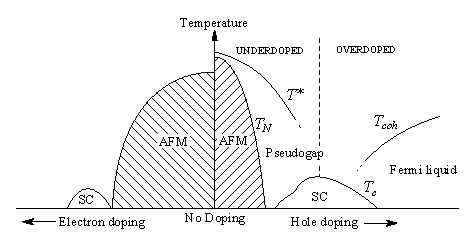
\includegraphics[scale=1.0]{Chapter-Introduction/Figures/ElecHolePhaseDiagram/ElecHolePhaseDiagram}
        \caption{A schematic phase diagram showing electron doped to the left and hole doped to the right. \ac{AFM} is the antiferromagnetic Mott insulating phase, SC is the superconducting phase. $T^*$, $T_N$, $T_c$ and $T_{\textrm{coh}}$ are the temperature scales for the pseudogap, \ac{AFM} state, superconductivity and coherent Fermi liquid phases respectively}
        \label{Fig:Intro:ElecHolePhaseDiagram}
    \end{center}
\end{figure}

\subsection{Mott insulating parent compound}

Starting at the middle of figure~\ref{Fig:Intro:ElecHolePhaseDiagram}, the parent compound materials at zero doping are thought to be Mott insulators i.e. the top most filled state on each lattice site contains one electron. In the conventional band picture this should be metallic since the bands are only partially filled, however when we consider a local picture of electrons, any movement of an electron to the neighbouring lattice site will cause an energetically costly double occupancy on one site and zero occupancy on another. This causes the electronic \ac{DOS} to become gapped around the Fermi surface and hence suppressed conduction. This is known as the Mott insulating state.

We find that the kinetic energy term is reduced when the ordering of the sites is antiferromagnetic since for any hopping to occur at all, the spins must be antialigned to avoid double occupancy of like spins. This region dominates the low doping portion of the phase diagram and remains antiferromagnetic until either the temperature is high enough to allow transitions from the Fermi energy to the states at the edge of the gap or the doping has introduced enough double occupancy electrons on lattice sites, which can move without the double occupancy energy cost, to overcome the insulating behaviour.

\subsection{Superconducting dome}

With increased doping, the antiferromagnetic state gives way to the superconducting dome at around $p=0.05$ which itself gives way to a Fermi liquid metallic state at a doping of around $p=0.3$. The maximum \Tc occurs at around $p=0.16$. Transitions from both the antiferromagnetic and the superconducting state are clearly second order thermodynamic with jumps in the heat capacity for example, however there are other regions in the phase diagram which are less well defined such as the pseudogap and the Fermi liquid crossover whose temperature scale can depend on the particular probe used and do not feature a clear order parameter.

\subsection{Coherent phase}

To the heavily overdoped side of the phase diagram, beyond the superconducting dome lies the coherent region where the system bears the hallmarks of a conventional metal. The implication is that correlations between electrons are sufficiently weak such that the mass enhanced quasiparticles of Landau's Fermi liquid theory are well defined, leading to conventional metal behaviour. A clear indication of this is a dominant $T^2$ term in the resistivity. Above this region we observe an anomalous additional contribution which has been modelled both with $T^2$ plus an additional linear term or by a $T^n$ term where $1 <= n <= 2$. This additional term has been observed in heavy Femrion materials and is often associated with proximity to a \ac{QCP}~\cite{Custers2003}.

\subsection{The pseudogap}

Above the antiferromagnetic region and the superconducting state is one of the most controversial regions of the phase diagram, the so called pseudogap phase. This is a region which was first demonstrated in 1989, just a few years after the discovery of the cuprate materials, by \ac{NMR} measurements performed at Bell labs~\cite{Warren1989}. A noticeable fall in the susceptibility occurred at a temperature significantly above $T_c$ which led to conclusion of possible spin pairing before the onset of bulk superconductivity\footnote{Cooper paired electrons in the singlet state have zero net spin hence they do not contribute to the susceptibility, whereas unpaired electrons do. Cooper pairing leads to a reduction in susceptibility, see for example neutron scattering plots.}. The question arose as to what the exact relation of the pseudogap is to the superconducting state --- is it a precursor state, from which superconductivity arises or is it a competing phase? --- and from a materials development point of view, to obtain higher $T_c$ should we be finding ways to suppress the crossover to the pseudogap state or encourage it?
\begin{figure}[htbp]
    \begin{center}
        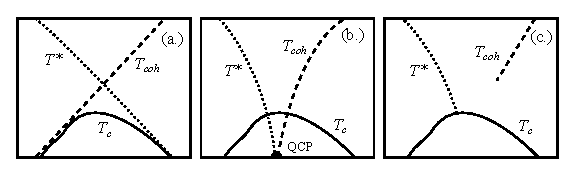
\includegraphics[scale=1.0]{Chapter-Introduction/Figures/PGScenarios/PGScenarios}
        \caption{Three scenarios proposed for the $T^*$ temperature scale behaviour. (a.) the pseudogap as the `precursor' state, (b.) as the `competing' state, (c.) and the `transition' scenario.}
        \label{Fig:Intro:PGScenario}
    \end{center}
\end{figure}
By finding where exactly the $T^*$ energy scale meets the superconducting dome, strong evidence can be found that supports one or the other scenario. However the problem lies in the type of probe used. Select spectroscopic measurements including \ac{STM}, \ac{ARPES} and Raman spectroscopy on materials of comparable $T_c$ values have found that the $T^*$ overreaches the superconducting dome entirely~\cite{Hufner2008}, meeting with the overdoped edge at $T=\unit{0}{\kelvin}$. This supports the precursor state theory illustrated in figure~\ref{Fig:Intro:PGScenario}~(a.) where $T^*$ and $T_{\textrm{coh}}$ cross to define a region which is below both temperature scales where the carrier are both coherent quasiparticles and paired leading to the superconducting condensate.

A second scenario is supported by measurements using bulk probes such as heat capacity, magnetic susceptibility and resistivity measurement have shown the $T^*$ energy scale drops into the top of the superconducting dome~\cite{Tallon2001}. This supports the scenario where the pseudogap is in competition with superconductivity for states at the Fermi surface. Once the pseudogap phase is suppressed, scattering from quantum fluctuations at zero temperature leads to the formation of the superconducting phase at a \ac{QCP} similar to that found in heavy fermion materials. This scenario is supported by the observation of linear scaling of the resistivity with temperature in the region above the superconducting dome which is a hallmark of proximity of a \ac{QCP}.
% Kondo is a competitive scenario which justified based on
% non-monotonicity of coherence as you move from the antinodes on the FS \cite{Kondo2009}

A third scenario is one where the pseudogap simply becomes the superconducting gap as it meets the top of the superconducting dome. However this scenario leaves hanging questions as to the roles of the pseudogap, $T_{\textrm{coh}}$ and other phenomena in the phase diagram which would need to be addressed theoretically. Moreover this picture is rendered less compelling by the observation in \ac{LSCO} of rapidly increasing, low temperature, normal state resistivity inside of the underdoped superconducting dome which implies the non-superconducting energy gap persists into this region.


\subsection{Previous work by the Bristol group}

Clearly lots of interesting physics is occurring in and around the superconducting dome and a solid understanding of this region is key to understanding the problem of high-$T_c$. Prof. N. Hussey has been involved in many efforts to shed light on the situation, of which, two key ones are highlighted here.

\subsubsection{Links between anisotropic scattering and $T_c$}

Simply measuring resistance along different axes gives an averaged scattering rate through all conduction paths and so to build a map of the angle dependent scattering rates, a different technique must be used. In \ac{ADMR} a strong persistent magnetic field is applied before resistance measurements are taken. The field serves two purposes; firstly, to suppress superconductivity so the normal state can be probed, secondly to confine the electrons to orbits perpendicular to the field. By detailed analysis of the change in resistance as the field is applied at various angles, a picture of the angle dependent scattering rate can be determined.

After performing measurements on samples of \ac{TL2201} with dopings ranging from strongly overdoped to slightly underdoped~\cite{Abdel-Jawad2006}, a trend emerged which is illustrated in figure~\ref{Fig:Intro:AnisotropyPhase}. 
\begin{figure}[htbp]
    \begin{center}
        \includegraphics[scale=0.9]{Chapter-Introduction/Figures/AnisotropyPhase/AnisotropyPhase}
        \caption{Schematic of how the scattering rate, $\Gamma$, the Fermi surface, $FS$, and the superconducting gap, $\Delta_g$ evolve with doping across the superconducting dome. Based on figure 1 in ref~\cite{Taillefer2006}. The dotted line in the scattering is the isotropic part.}
        \label{Fig:Intro:AnisotropyPhase}
    \end{center}
\end{figure}
Here the scattering rate within the $ab$-plane, $\Gamma$, was found to be composed of two terms; an isotropic term which remained constant with doping (dotted circle) and an anisotropic component which scaled with the superconducting gap, $\Delta_g$. Moreover it was found that the superconducting gap and the anisotropic scattering rate both shared the same shape, being `d-wave'. This further ties to \ac{ARPES} measurement which show that the on the underdoped side of the superconducting dome there is a pronounced change in the Fermi surface where at the antinodal points of $\Gamma$ (and $\Delta_G$) the spectral weight disappears~\cite{Norman2010} i.e. coherent particles are lost away from the regions of strong scattering.

%It changes from a single large hole band of volume $1+p$ to series of small regions of electron and hole Fermi surface of total volume $p$.

\subsubsection{T-Linear behaviour in the superconducting dome}

Previous high-field transport measurements on Sr doped \ac{LSCO}~\cite{Cooper2009} gave key insights into the nature of the T-linear term as it entered the superconducting term on the overdoped side. In particular it showed that the T-linear term did not funnel down to a point (figure~\ref{Fig:Intro:CooperTLinear}) as is typical of \ac{QCP} behaviour but instead spread out into the superconducting region. Intrigued as to this unexpected behaviour, we looked to repeat the measurements on \ac{BSCO} which can be doped far more widely without divergence in the resistivity so that we could then see how the T-linear term progressed on the underdoped side, where $T^*$ is undisputed.
\begin{figure}[htbp]
    \begin{center}
        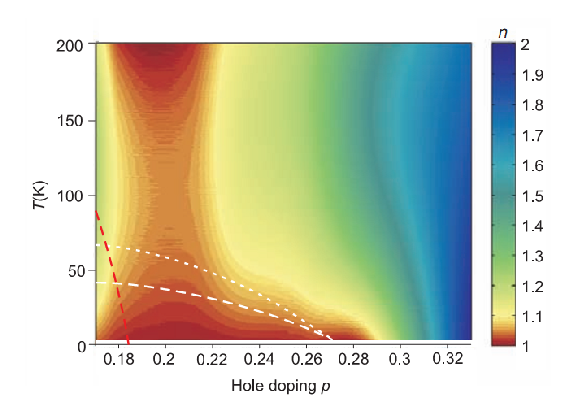
\includegraphics[scale=0.8]{Chapter-Introduction/Figures/CooperTLinear/CooperTLinear}
        \caption{Plot of the $T^n$ term in the fitted field suppressed normal state of Sr doped \ac{LSCO} showing the $T$-linear term extending throughout the superconducting dome and not to a single \ac{QCP}. Taken from Cooper \etal~\cite{Cooper2009}}
        \label{Fig:Intro:CooperTLinear}
    \end{center}
\end{figure}
Performing measurements which would shed light onto which of the scenarios shown in fig~\ref{Fig:Intro:PGScenario} is most likely to be correct formed the original motivation for the investigation of \ac{BSCO} through transport measurements. 

A second reason for the study of \ac{BSCO} in particular is that it's van-Hove singularity occurs at a different doping --- further from optimal doping --- than \ac{LSCO}. Should similar behaviour be found then we can confidently claim that the unusual \ac{QCP} behaviour is not due to proximity to the changeover in hole-like to electron-like Fermi surface and is likely universal to all cuprates. 

\ac{BSCO} also demonstrates transport behaviours which are consistent with other high-$T_c$ cuprate materials. For example, from \ac{MR} measurements it demonstrates a similar maximum in the underdoped $d\rho_{ab}/dT$ curve as underdoped YBCO~\cite{Ando1999}. On the overdoped side, \ac{BSCO} demonstrates a monotonic upward trend in $d\rho_{ab}/dT$ with increasing temperature similar to what has been observed in Tl$_{2201}$ and \ac{LSCO}~\cite{Ando1999}.

During the course of the investigations however, it became apparent that even with field strengths of up to \unit{60}{\tesla} in pulsed fields, the upper critical field, $H_{\textrm{c2}}$ of many of the sample at key temperatures could not be reached. However, field strengths were generally strong enough to recover $B$-Linear behaviour in the Hall component.

Previous Hall measurements have been performed on \ac{BSCO} by Ando \etal~\cite{Ando1999, Ando2000} which are shown for comparison in the results section. However these results do not go to low temperatures, being restricted by the onset of superconductivity. Our own results used high field measurements at \ac{LNCMI} and \ac{HFML} to suppress superconductivity and examine the low temperature regions in detail. Moreover our samples are focused on the overdoped region which complements the underdoped data set presented in the Ando papers.

% Motivation

% Lograithmic divergence of scattering rate observed in cuprates which
% begins at critical doping and increases as become more underdoped.
% However common factor of cuprates (Y123, Tl2201, LSCO) is a change of
% Fermi surface (in LSCO at least) from hole to electron leading to a
% van Hove singularity(?) which occurs similar to hwere would expect the
% insulating crossover. This does not occur in BSCO however until
% around p=0.2\cite{Hashimoto2008}. If the \alpha^2 term takes off
% earlier for BSCO\cite{Hussey2011a} is good
% evidence that is due to the proximity to van Hove rather  than Moot
% insulator transition.\cite{Ono2000}


% \section{Mott physics}

% The Hubbard model takes the relatively simple and solvable tight-binding model and introduces an Anderson term which raises the energy for double occupancy by an amount $U$, known as the `Hubbard U'. This simple change deeply enriches the physics with one of the outcomes being the existance of the Mott insulating state which occurs when each lattice site is half filled with a single electron. The energy cost for an electron to hop to an adjacent site is so high that it locks the electrons in place, preventing effective conduction. Introducing holes (or electrons) allows once again hopping to take place and the eigenstates are no longer entireley localised.




\section{Fermi surface nesting as a pairing mechanism}

The charge carrier in a superconducting condensate is a Cooper pair - a quasi-particle comprising of a bound state of two electrons or two holes with opposite spin and momentum. Evidence for this configuration arises as a natural result of the Ginzberg-Landau model which, when applied to a superconducting system, gives the charge of the quasi-particle carriers as $2e$, where $e$ is the charge of an electron. Given that due to their like charges two free electrons repel, it is natural to ask what could overcome the electromagnetic force to cause these electrons to remain bound in this quasi-particle state.

Bardeen, Cooper and Schreiffer established much of the theoretical basis --- from which the Ginzberg--Landau model can be derived --- in \textit{BCS theory} (named after the authors) and within the framework of BCS theory, wrote a 1957 paper\cite{Bardeen1957} detailed a pairing mechanism known as the \textit{BCS model} which would explain how these electron remained bound together. The model is based around the concept of phonons scattering off ions which well suited the superconducting materials known at the time. Phenomenologically, the mechanism of attraction is straightforward. Electrons moving through a crystal lattice attract ions on the lattice sites. These heavy ions respond slowly and are drawn in \textit{behind} the electron. This has the effect of both screening the negative electron charge as well as providing an attractive positive potential for any electron following the original electron. The net effect is the leading electron draws the following electron in its wake, thus coupling them with one another. The wavelike distortion of the ions in the lattice can be considered as a phonon, and the interaction between the electrons and the lattice can be modelled as electron--phonon--electron scattering.

The BCS model on top of BCS theory accurately describes what we now know as \textit{conventional superconductivity}, that is pairing which forms a spin-singlet state ($S=0$) and which has zero orbital angular momentum ($L=0$). It was not until the discovery of superfluidity\footnote{Superfluidity and superconductivity share much of the same physics although rather than electrons or holes pairing, molecules pair instead. Parallels betwen the two are discussed in ref.\cite{Annett2010}} in $^3$He in 1972\cite{Osheroff1972} that it became apparent that there may exist forms of pairing that resulted in spin-triplet pairing state ($S=1$) with $L>0$. This was later confirmed when superconducting analogues were found in the form of heavy Fermion materials. What really spurred the explosion in interest though was the 1986 discovery by Bednorz and M\"uller\cite{Bednorz} of high transition temperature (\Tc) superconductivity in the cuprates and, more recently, the `pnictides' by Kamihara et al.\cite{Kamihara2008}. The cuprate class of materials that Bednorz and M\"uller found to be superconducting have \Tc~s far in excess of any previously known superconducting materials and although the BCS model phonon pairing may play a part, the predominant pairing mechanism in the \highTc materials is likely to be something else entirely.

\subsection{The case against conventional superconductivity in \highTc}

There is a great deal of evidence in the literature for non-BCS model pairing in the \highTc and heavy Fermion materials. Although the pairing wavefunction cannot be measured directly with current techniques, experiments indirectly infer \textit{unconventional} i.e. non s-wave, BCS-model, characteristics. For example, analysis on penetration depth measurements of YBa$_2$Cu$_3$O$_{7-\delta}$ show power law behaviour\cite{Annett1991}, indicating that there exists states within the momentum averaged gap. SQUID measurements and Josephson tunneling experiments on the same material have confirmed alternating phase of the condensate wavefunction which points strongly to \DxTwoyTwo--wave symmetry\cite{VanHarlingen1994} (see also refs. therein). As for other cuprate materials, specific heat measurements on \BSCO\cite{Wang2011}, as well as peentration depth measurements on LSCO\cite{Froehlich1996} have also proved consistant with $d$-wave pairing. 

More evidence against conventional superconductivity include the unusual normal state (i.e. non-superconducting) state properties of the cuprates and heavy Fermion materials. The BCS model is grounded in Landau Fermi liquid theory which models interacting itinerent electrons with quasiparticles of heavier effective mass than ordinary electrons and holes. A hallmark of Fermi liquid behaviour is a $T^2$ dependence of the resistance, however experiments on the cuprate La$_{2-x}$Sr$_{x}$CuO$_4$\cite{Cooper2009} and a heavy Fermion material\cite{Custers2003} have demonstrated fractional power law behaviour, $T^\gamma$ where $1 < \gamma < 2$, at temepratures above the superconducting transition. Given that the Fermi liquid model breaks down in these examples, it follows that the BCS-model also is likely on shaky ground for these materials.

There are several arguments against phonons as the sole pairing mechanism in the pnictide case, Boeri et al.\cite{Boeri2008} and Mazin et al.\cite{Mazin2008} present calculations showing that the magnitude of the phonon pairing strength is not adequate for the high \Tc values attained in LaAsOF, Haule et al.\cite{Haule2008} note in the same material that the gradient of the density of states (DOS) at the Fermi level is such that you would expect an increase in DOS and hence \Tc with hole doping if the BCS model held, however the reverse is true. Non Fermi-liquid behaviour was demonstrated in the \BaFePAs series\cite{Jiang2009,Kasahara2010} and evidence for nodes in the gap function have been found in LaFePO\cite{Fletcher2009} and the \BaFePAs series\cite{Zhang2011,Yamashita2011a,Suzuki2011} although not in % TODO

It is interesting to note that Unlike the cuprates which universally show a \DxTwoyTwo gap symmetry, the pnictide materials are note all alike. As a result, it may prove that the nature of the supercondcutivity may not be universal amongst the pnictide materials. Irrespective of this, there is no evidence for BCS model pairing in the pnictide materials and in many cases, BCS pairing has been shown to be insufficient.


\subsection{Spin-fluctuations}

Soon after the discovery of the pnictide materials, a possible pairing mechanism was proposed based on spin density wave fluctuations. The original paper suggested a $s_{\pm}$ gap symmetry which does not feature any nodes however 

\subsection{Pnictides}

Some arguments against the BCS theory of pairing \cite{Haule2008,Yndurain2009,Mazin2008} based on arguments of 

FS nesting not the only cause of spin-fluctuations, also can be caused by frustrated superexchange for example % TODO

Spin fluctuations mediate a repulsive interaction between Cooper pair candidates.

The anisotropic BCS equations specify that repulsive coupling between carriers can be pairing provided the order parameter changes sign over the coupling vector.


There are several proposed mechanisms presently on offer including charge fluctuations resulting in large ion polarisation \cite{Berciu2009}, however this was contested by Mazin and Schmalian\cite{Mazin2009}.


Of these theories, the one with arguably the most traction at present is that of spin-fluctuation mediated pairing. 

TODO: What actually is the cause of the attraction in the nesting picture? ... Spin fluctuation intereaction in real space is approximately propoprtional to the dipole interaction $V=-\mu . \mu \chi(r)$\cite{Bergemann2003} 



Strong correlations - the interaction energy is much greater than the kinetic energy for the states
When correlations present, Cooper pairs are assumed to be pairs of Landau quasiparticles


\subsection{Susceptibility}
    \label{Sec:Intro:NestingSusceptibility}

A commonly used measure of the nesting condition is the Lindhard susceptibility function. This is often quoted as,
\begin{equation}
\chi_0(\vec{q}, \omega) = \lim_{\eta \to 0} \sum_{\vec{k}}\sum_{l,l\prime}\frac{f(\epsilon_{\vec{k}+\vec{q},l\prime}) - f(\epsilon_{\vec{k},l})}{\epsilon_{\vec{k}+\vec{q},l\prime} - \epsilon{\vec{k},l} - \hbar\omega - i\eta}|\langle \vec{k}+\vec{q},l\prime \mid  V \mid \vec{k},l \rangle|^2
\label{Eqn:Intro:Lindhard}
\end{equation}
respectively. The numerator term contains two Fermi functions ($f(\epsilon) = 1/(\exp{\frac{\epsilon - \epsilon_F}{k_B T}} + 1)$) where $\epsilon$ and $\epsilon_F$ are the state energy and the Fermi energy respectively and $k_BT$ is the usual Boltzman energy conversion factor. These Fermi functions ensure that the susceptibilty is finite for states which scatter across the Fermi energy and zero if they do not. They also smear the calculations as a function of temperature. The final term in the denominator is an artefact of the adiabatic approximation used to calculate the perturbation. The completed approximation takes the limit of $\eta \to 0$ which results in an expression for the imaginary part of Lindhard susceptibility, $\mathcal{Im}(\chi_0) \propto \delta(\epsilon_{\vec{k}+\vec{q},l\prime} - \epsilon{\vec{k},l} - \hbar\omega)$ which, in a continuous calculation, results in resonances at excitations which match the difference in energies between states. However, in this thesis, the energy dispersions used to determine nesting conditions are not continuous and instead are based on discrete energies obtained from DFT calculations. As such $\eta$ will have to remain finite in order to broaden the delta function into a Lorentzian with width comparable to the energy differences between the discrete points -- the net result of this will be loss of some fine structure. The third term in the denominator corresponds to the excitation energy of the perturbing field with $\omega$ corresponding to the temporal frequency of the field. The first sum in the Lindhard function is over all $\vec{k}$ states in the first Brillouin zone. The DFT calculations do not provide values for all $\vec{k}$ states, instead a fairly coarse mesh evenly distributed over the Brillouin zone is used. The second sum combines each energy band. In practice only bands that lie close (within the adiabatic or temeprature broadening) to the Fermi energy need to be included in the calculations.

Peaks in this function correspond to scattering of states which cross the Fermi energy yet remain close to the Fermi energy.  We can derive this function by modelling an oscillatory perturbing field on a system. To solve to get an expression for the second order perturbation, we make the adiabatic limit approximation (i.e. the perturbing potential is gradually increase from zero at $t=\infty$ to $v$ at $t=0$).

The real and imaginary parts of equation \ref{Eqn:Intro:Lindhard} are,
\begin{align}
\chi_0(\vec{q}, \omega)\prime &= \lim_{\eta \to 0} \sum_{\vec{k}}\sum_{l, l\prime}\frac{(\epsilon_{\vec{k}+\vec{q},l\prime} - \epsilon{\vec{k},l} - \hbar\omega) f(\epsilon_{\vec{k}+\vec{q},l\prime}) - f(\epsilon_{\vec{k},l})}{(\epsilon_{\vec{k}+\vec{q},l\prime} - \epsilon{\vec{k},l} - \hbar\omega)^2 + \eta^2}|\langle \vec{k}+\vec{q},l\prime \mid  V \mid \vec{k},l \rangle|^2 \\
\chi_0(\vec{q}, \omega)\prime\prime &= \lim_{\eta \to 0} \sum_{\vec{k}}\sum_{l, l\prime}\frac{-\delta f(\epsilon_{\vec{k}+\vec{q},l\prime}) - f(\epsilon_{\vec{k},l})}{(\epsilon_{\vec{k}+\vec{q},l\prime} - \epsilon{\vec{k},l} - \hbar\omega)^2 + \eta^2}|\langle \vec{k}+\vec{q},l\prime \mid  V \mid \vec{k},l \rangle|^2 \\
\end{align}
respectively.

Although knowledge of the susceptibility is useful to model, for example, neutron scattering measurements, for our purposes we will use it to demonstrate the strength of particular nesting vectors in our example materials. For this reason we make the assumption that the transition matrix elements are unity. This assumption greatly simplifies the calculations at the cost of some structure and as such should be borne in mind that the results are somewhat broad and qualitative.


TODO: How does susceptibility tie in with nesting?
TODO: Lindhard susceptibility is a time dependent perturbation in the adiabatic limit to what? Adiabatic limit is where the pertubation time-frame is slow c.f. the unperturbed time-frame 
TODO: imaginary factor corresponds to the decay rate of the state
TODO: energy(susceptibility) is broadened by the decay rate




% The Stoner condition of $\mathcal{N}_0 I > 1$ -- where $\mathcal{N}_0$ is the density of states at the Fermi energy and $I$ is the molecular field constant, that scales the magnetism given a field -- indicates an energy instability\cite{Kubler2000}



\section{The pseudogap vs. the coherent state}

The phase diagram for the cuprates, when hole doping is the tuning parameter, appears to be universal, however, at the time of writing, is somehwhat more complicated than that of a typical pnictide\footnote{In general there is more variation in the phase diagram amongst pnictide materials, however there are less features in these diagrams when compared to the cuprates}. With reference to the schematic cuprate phase diagram shown in figure~\ref{Fig:Intro:UniversalCupratePhaseDiagram} we see several temperature scales that may or may not be of interest to the underlying causes of \highTc superconductivity.
\begin{figure}[htbp]
    \begin{center}
        
\includegraphics[scale=0.7]{Misc/TODO}
        \caption{A schematic phase diagram of a series of hole-doped cuprates}
        \label{Fig:Intro:UniversalCupratePhaseDiagram}
    \end{center}
\end{figure}
From the standpoint of conventional superconductivity, the first striking feature is the proximity of an antiferromagnetic phase to the superconducting region. Even without actual temperature labels, it becomes clear that if this was a phonon mediated superconductor, the pairing must be strong in order to overcome the strong spin-density wave scattering that results in the anitferromagnetic state.

Another interesting region, one that is not present in the pnictides, is that below the $T^*$ temperature scale on the underdoped side of the superconducting dome. In this region, an energy gap opens up in the excitation spectra but without any sign of the Meissner effect. This region is known as the \textit{pseudogap}. Some aspects of the pseudogap lead us to believe that it is closely related to the superconducting gap such as the fact that it shares the gap symmetry and is of a similar magnitude, and there have been proposals that the pseudogap is a precursor state to superconductivity TODO. However research involving the Bristol group has shown evidence that phase fluctuations rather than the pseudogap in particular are the neceesary precursors for the cuprate superconducting condition\cite{Rourke2011}.

\subsection{Anisotropic scattering}





\section{Cuprate doping determination}




\chapter{Theory}


\section{De Haas-va Alphen oscillation}

In this section the phenomenon of \ac{dHvA} oscillations is described. It is not immediately apparent how a ramping magnetic field could cause oscillations in such a wide range of parameters but Lifshitz and Kosevich established their eponymous equation based on a theoretical basis set out by Landau which was then used to characterise the Fermi surface of many metals and establish the field of `Fermiology'. Strictly, only the oscillations in magnetisation are \ac{dHvA} oscillations and those in resistance are called Shubnikov-de Haas oscillations. Nonetheless they both originate from the same underlying phenomena of oscillations in the system energy.

\subsection{Overview}

For metals, the majority of the interesting physics occurs at the Fermi level and, provided Fermi liquid theory holds true, the electrons at the Fermi level can be modelled to a high degree of accuracy with the Sommerfeld model --- that is a Fermi gas of non-interacting electrons in an infinite box. When a magnetic field is applied, the electrons have their usual grid pattern distribution of plane wave k-vectors rearranged such that the electrons move around orbital and helical paths. These rearranged k-vectors form a set of concentric tubes, known as Landau tubes, whose cross-sectional area, $a$, perpedicular to the field is given by the Onsager relation:\footnote{Derivations of the Onsager relation are given in several textbooks including pg. 32 of Schoenberg\cite{Schoenberg1984} and pg. 272 of Ashcroft \& Mermin\cite{Ashcroft1976}.} 
%%
\begin{equation}
\label{Eqn:Theo:Onsager}
\textit{a}_{k_{\perp}} = (r + 1/2)\frac{2\pi e B}{\hbar}
\end{equation}
%%
where $r$ is a quantisation number that sets apart each tube. We can see from the relation that as $\vect{B}$ increases, so does the cross-sectional area of the tubes. As the magnetic field is ramped, successive tubes periodically pass the Fermi surface causing a spike in the \ac{DOS} at the Fermi level and also oscillations in the energy o the ssytem, $E$, which, for geometric reasons explained in the next section, are far stronger at the maximumal and minimal (extremal) areas of Fermi surface. Thermodynamic quantities such as magnetic susceptibility ($\chi = \partial E/\partial B$) and heat capacity ($C_{V} = \partial^2E/\partial T^2|_{V}$) or quantities that depend on the \ac{DOS} at the Fermi level such as electrical resistance all oscillate as the field is ramped. Oscillations in the susceptibility are known as \ac{dHvA} oscillations, oscillations in the resistivity are known as Shubnikov-de Haas oscillations.

 We can relate the `frequency' $F$ (measured in $tesla$\footnote{n.b. that it is \textit{tesla} and not \textit{tesla$^{-1}$} because, as we shall see later, the oscillations are actually periodic in $1/B$ and \textit{not} $B$ so their frequency counterpart is measured in \textit{tesla}.}) that the tubes pass the Fermi surface to the extremal Fermi surface area using the following application of the Onsager relation,
%%
\begin{equation}
\textit{a}_{k_{\perp}} = \frac{2\pi e }{\hbar}F
\end{equation}
%%
By varying the direction of the field we can obtain a series of maximal and minimal Fermi surface areas in a variety of orientations in order to build a profile of the Fermi surface topology and size. In practice, there are many possible variations that might fit the model based on areas of cross-sectional slices alone and so typically ab-initio \ac{DFT} calculations --- described in sections~\ref{Sec:Theo:Dft} and~\ref{Sec:Exp:Dft} --- are employed to provide a basis which can be tweaked based on the constraints from the measurements. 

A more detailed analysis of this process follows, beginning with an illustrative mathematical treatment for oscillations in the magnetisation.

\subsection{Exploring the origin of the oscillations}

We begin by calculating the degeneracy of the Landau tubes i.e. the number of electron states per tube. Because the states under a magnetic field are a one-to-one rearrangement of the states with no field, we can use the Sommerfeld number of states per unit k-space ($V/4\pi^3$) to determine the degeneracy. From the Onsager relation (eqn.\ref{Eqn:Theo:Onsager}) we see that the additional area for successive tubes is $\Delta a_{k_{\perp}}  = 2\pi e B/\hbar$ which we can convert to a volume by integrating over $k_{\perp}$. This gives a degeneracy per tube therefore of,

\begin{equation}
D_{\textrm{tube}} = d k_{\perp}\left(\frac{2\pi e B}{\hbar}\right)\left(\frac{V}{4 \pi^3}\right) = \frac{eBVdk_{\perp}}{\hbar 2\pi^2}
\end{equation}

We continue by writing an expression for the energy of the system, $E$ by summing the energies of the states that lie beneath the cross-sectional area defined by the Fermi surface ($a_{k_\perp F}$) for a given $k_\perp$. To do this, we use the Onsager equation to determine $R_\perp$ --- the number of Landau tubes below the Fermi surface at this cross-sectional slice. We then multiply this by the degeneracy of the tubes, $D$ and the energy for states on that particular Landau tube, $\epsilon_r$,
%%
\begin{equation}
\label{Eqn:Theo:OscillateE}
E = D\sum_{r}^{R_\perp}\epsilon_r = \frac{eBVdk_\perp}{\hbar 2 \pi^2}\sum_{r}^{R_\perp}\epsilon_r
\end{equation}
 where,
\begin{equation}
R_\perp = \textrm{floor}\left[\frac{a_{k_\perp F}\hbar}{2\pi e B} - \frac{1}{2}\right]
\end{equation}
%%
To complete the above equation, we need an expression for the energies of each of the Landau tubes. The procedure for the free electron case is to insert the canonical momentum (i.e momentum of a free electron in a magnetic field) into the non-interacting Schr\"odinger equation and solve to obtain the following eigenvalues for the energies on the Landau tubes. Full derivations can be found in several textbooks\footnote{See for examples pg. 32ff. in Schoenberg\cite{Schoenberg1984} or pg. 148ff. in Blundell\cite{Blundell2001}.} and so will  not be repeated here. Below is the expression for the energy eigenvalues,
%%
\begin{equation}
\epsilon_r=(r+1/2) \hbar \omega_c + \frac{\hbar^2 k^2}{2m_0} \textrm{\hspace{0.2cm}where,\hspace{0.2cm}} \omega_c = \frac{eB}{m_0}
\end{equation}
%%
and is known as the \textit{cyclotron frequency}. The summation term in equation\ref{Eqn:Theo:OscillateE} can now be written,
%%
\begin{align*}
\sum_r^{R_\perp}\epsilon_r &= \sum_r^{R_\perp}\left( (r+1/2) \hbar \omega_c + \frac{\hbar^2 k^2}{2m_0} \right) \\
    &= \frac{\hbar eB}{m_0}\sum_r^{R_\perp}r + \frac{\hbar eB}{2m_0}\sum_r^{R_\perp}1 + \frac{\hbar^2 k^2}{2m_0}\sum_r^{R_\perp}1 \\
    &= \frac{\hbar eB}{2 m_0} R_\perp(R_\perp + 1) + \frac{\hbar eB}{2m_0}R_\perp + \frac{\hbar^2 k^2}{2m_0}R_\perp \\
    &= \frac{\hbar eB}{2m_0}R_\perp^2 + \left(\frac{\hbar eB}{m_0} + \frac{\hbar^2 k^2}{2m_0}\right)R_\perp
\end{align*}
%%
which can be expanded out and finally substituted back into equation\ref{Eqn:Theo:OscillateE} to finally obtain,
%%
\begin{equation}
\label{Eqn:Theo:OscIllustration}
E = \frac{e^2Vdk_\perp}{4\pi^2m_0}B^2\left[R_\perp^2 + 2R_\perp + \frac{\hbar k^2}{e}\frac{1}{B}R_\perp\right]
\end{equation}
%%
Key to the above relation is that, although $R_\perp$ is inversely proprtional to $B$, it remains discrete. This gives rise to the saw-tooth like function shown in figure~\ref{Fig:Theo:EnergyOscillations} for some typical experimental parameters. Also plotted is the fuction against $1/B$ where we can clearly see that the oscillations are periodic in inverse field hence the frequency being measured in tesla$^{-1}$.
%%
\begin{figure}[htbp]
    \begin{center}
        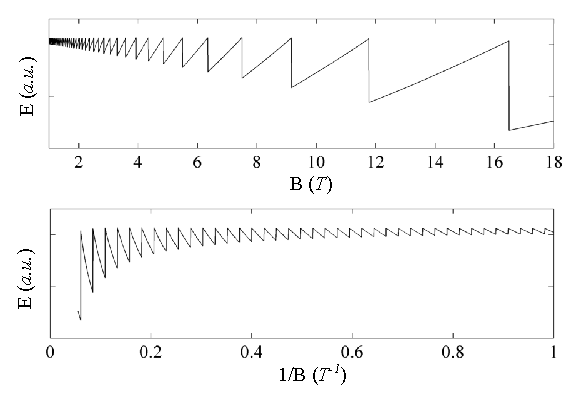
\includegraphics[scale=0.9]{Chapter-Theory/Figures/TheoreticalOscillations/TheoreticalOscillations}
        \caption{Theoretical energy oscillations for a Fermi surface orbit which is 5\% of a \unit{5}{\angstrom} cubic \ac{BZ} between \unit{1-18}{\tesla}. Kinetic energy term is taken to be for an electron at a level half the size of the Fermi surface.}
        \label{Fig:Theo:EnergyOscillations}
    \end{center}
\end{figure}

The above is not a rigourous derivation but is nonetheless illustrative of the origin of the oscillation in the system energy and how any thermodynamic value which depends on the energy of the system oscillates as a function of field. To continue we need to include correction factors to the oscillation amplitude due to finite electron scattering rates ($A_D$), temperature ($A_T$), Zeeman splitting of spins ($A_s$), doping ($A_{\textrm{dop}}$), mosaicity ($A_{\textrm{mos}}$), warping of the Fermi surface ($A_{\textrm{warp}}$) as well as adjustments due to the fact that the parameter measured was torque of the sample in a field and not the energy or magnetisation directly ($A_{\Gamma}$). For this, we turn to a more solid foundation that was put forward by Lifschitz and Kosevitch and presented by Schoenberg.

\subsection{\acl{LK} equation}

The derivation for the full expression for the Landau thermodynamic potential, $\Omega$\footnote{Formally defined as the energy in a open system that is in thermal contact with its surroundings}, begins in a similar way to the previous illustrative example but frames the sawtooth-like function above as a more mathematically manageable Fourier decomposition which also conveniently makes the technique highly amenable to Fourier analysis. For this reason the equation below features higher harmonics which are denoted with the identifier $p$.
%%
\begin{equation}
\Omega = \left(\frac{e}{2\pi\hbar}\right)^{\frac{3}{2}}\frac{e\hbar B^{\frac{5}{2}}}{m_0 \pi^2}\left| \frac{\partial^2 a_{\textrm{ext}}}{\partial k^2_\perp}\right|^{-\frac{1}{2}}\sum_{p=1}^{\infty}p^{-\frac{5}{2}}A_{\textrm{tot}}\cos\left[2\pi p\left(\frac{F}{B} - \gamma\right)\pm\frac{\pi}{4}\right]
\end{equation}
where,
\begin{equation}
A_{\textrm{tot}} = A_T A_D A_s A_{\Gamma} A_{\textrm{mos}} A_{\textrm{dop}} A_{\Delta B}
\end{equation}
%%
The above equation and derivatives of it are known as the \ac{LK} equation. To obatin the magnetisation the differential with respect to $b$ is taken to get,
%%
\begin{equation}
M = \left(\frac{e}{\hbar}\right)^{\frac{3}{2}}\frac{e\hbar F V B^{\frac{1}{2}}}{m_0 \pi^\frac{5}{2}\sqrt{2}}\left| \frac{\partial^2 a_{\textrm{ext}}}{\partial k^2_\perp}\right|^{-\frac{1}{2}}\sum_{p=1}^{\infty}p^{-\frac{3}{2}}A_{\textrm{tot}}\sin\left[2\pi p\left(\frac{F}{B} - \gamma\right)\pm\frac{\pi}{4}\right]
\end{equation}
%%
To attain the above equations, it was necessary to perform an integral over $k_\perp$\footnote{Similar to the integral in the toy equation from the previous section} which results in a parameter for an extremal Fermi surface orbit area perpendicular to the field given by $a_{\textrm{ext}}$. 

\subsubsection{Attenuation for non-extremal orbits}

Only the extremal (i.e. the largest and smallest) magnetically induced orbits contribute significantly to oscillations in the system energy. This is because $F$ represents a phase factor in the \ac{LK} equation and at the extremal points $dF/dk_\perp=0$ meaning more orbits near extrema are in phase. However it is not immediately clear how much stronger the oscillations from the extremal orbits will be in comparison to other orbits. Figure~\ref{Fig:Theo:ExtremalPhases} shows examples of the strengths of the oscillations after integrating over a distribution of phases shown in the insets.
%%
\begin{figure}[htbp]
    \begin{center}
        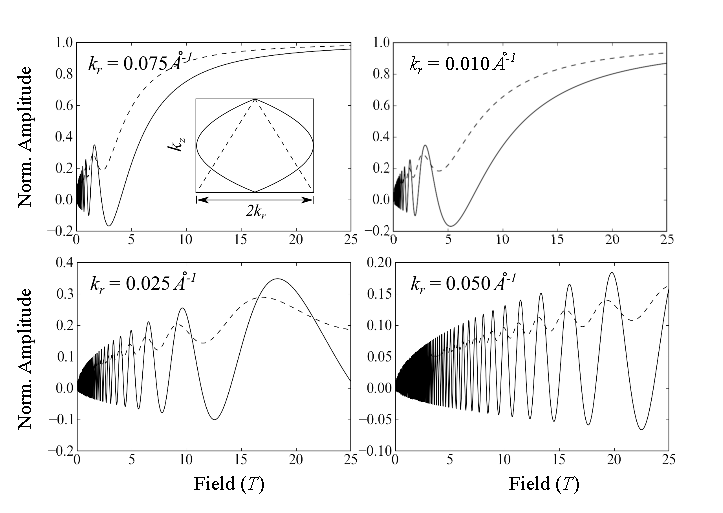
\includegraphics[scale=0.8]{Chapter-Theory/Figures/ExtremalPhases/ExtremalPhases}
        \caption{The sum of 1000 cosines with phase dispersions shown in the insets. Dashed line represents an extremal dispersion, solid lines a spread of linear dispersions and dotted line represent a non-extremal inflection point. Top left, top right and bottom left panels have phase distributions that are scaled from $0$ to $\sim1$, $\approx10$ and $\approx100$ Landau tube `wavelengths' respectively.}
        \label{Fig:Theo:ExtremalPhases}
    \end{center}
\end{figure}
%%
The panels each show the phases from the distributions taken over a range of scales, and it is clear that the phase cancellation is more acute for longer scales. This makes sense if we consider that the Landau tubes passing the Fermi surface are a oscillatory measurement probe like any other and so will be wavelength limited. That is, if the difference between the outermost and innermost orbits are of the order of the Landau tube spacing as is passes the Fermi surface, then the oscillations will be difficult to pick out. Interestingly this also places a limit on the maximum field that can be used to probe a Fermi surface since, according to the Onsager relation, the larger the field the larger the spacing between tubes. In practice this is simply $\Delta a_{k_\perp}$ which means that in terms of $F$, the resolutions is simply the field (i.e. $\sigma_F \sim \unit{18}{\tesla}$ for the Yellow magnet at Bristol). 

A final point is that it is not strictly extremal points that contribute significantly to the oscillations, but also inflected stationary points as shown in the last panel of figure~\ref{Fig:Theo:ExtremalPhases} so on could imagine a pathological stepped Fermi surface that would feature several strong orbital oscillations which would not be at turning points.

Variations in the phases can also be put into practice to model the various effects on the \ac{LK} equation listed towards the end of the previous section. These can be manifest by convolving an appropriate phase distribution function with the cosine oscillatory term. It can be shown\footnote{See for example, Schoenberg pg 57--59.\cite{Schoenberg1984}} that this convolution results in a relatively simple multiplication factor --- hence the various $A$ factors listed in the \ac{LK} equation which we expand upon below.

\subsubsection{Attenuation due to temperature}

To find the appropriate phase distribution function for the temperature dependence we start with the Fermi distribution,
\begin{equation}
\label{Eqn:Theo:FermiFunction}
f(\epsilon) = \frac{1}{\exp\left((\epsilon-\mu)/kT\right) + 1}
\end{equation} 
The differential of this distribution results in the broadening function (which is proportional to the probability that the Fermi energy $\mu$ is between $\epsilon$ and $\epsilon + d\epsilon$),
\begin{equation}
  P(\epsilon < \mu < \epsilon + d\epsilon) \propto \frac{d\epsilon}{2kT(1 + \cosh[(\epsilon - \mu)/kT])}
\end{equation}
This is convolved across the Fermi energy to smear it and also the phase through the parameter $F$. The details of how this is done is given in Schoenberg pg. 59ff~\cite{Schoenberg1984} with the end result is given by,
\begin{equation}
\label{Eqn:Theo:TemperatureTerm}
  A_T = \frac{X}{\sinh(X)} \textrm{\hspace{0.3cm} where,\hspace{0.3cm}} X = \frac{2\pi^2pkT m^*_T}{e\hbar B}
\end{equation}

The above factor includes $m^*_T$, the \textit{thermal effective mass} as a term in a function of $T$. As a consequence, by studying the temperature dependence of the amplitude it is possible to get a measure of $m^*_T$ of the electrons at the extremal orbit. Techniques for doing this are discussed in section~\ref{Sec:Exp:ExtractingEffMassTemperatureDependence}.

The effective mass determined in this way is enhanced subject to the same interactions as in heat capacity experiments --- i.e. electron-phonon interactions and spin symmetric correlations --- but are probed for a particular Fermi surface orbit, whereas heat capacity is bulk averaged. As we will see later the mass enhancement is is different to that from spin measurements. For more one this see Rourke \etal\cite{Rourke2010b} and references therein.

\subsubsection{Attenuation due to finite quasiparticle lifetime}

The \textit{Dingle factor}, $A_D$, is due to the finite lifetime, $\tau$, of the electron quasiparticles due to scattering. Because of this time scale, there is a smearing of the electron energy through the uncertainty principle with a broadening which is approximately Lorentzian in shape. If we assume $\tau$ does not change with energy\footnote{This is not the case, but at most only a few Landau levels contribute to a particular oscillation and if we assume that the energy does not vary too much between subsequent levels then the assumption is a good one}, then this can be modeled as a smearing of the Fermi level such that the broadening function is,
\begin{equation}
  P(\epsilon < \mu < \epsilon + d\epsilon) \propto \frac{d\epsilon}{(\epsilon - \mu)^2 + (\hbar/2\tau)^2}
\end{equation}
and such that after the routine Fourier transform, the end relation is given by,
\begin{equation}
  A_D = e^{-\pi p m_b/e B\tau} = e^{-\pi p/\omega_c\tau} 
\label{Eqn:Theo:DingleTerm}
\end{equation}
The exponent in the above can be thought of as the number of orbits the electron has completed (i.e. each harmonic $p$ is another successive orbit) divided by the expected number of orbits it will complete, so evidently we expect to see the higher harmonics having an exponentially lower amplitude. The term $m_b$ refers to the \textit{band mass} which will be discussed in detail later on. 
%The mass term here is \TODO{How is it coupled as Tony described?}

\subsubsection{Attenuation due to spin splitting}

Applying a magnetic field causes a Zeeman splitting of energy levels of amgnitude,
\begin{equation}
  \Delta\epsilon = \frac{g e \hbar B}{2 m_e}
\end{equation}
where $m_e$ is the free electron mass and $g$ is a factor that is $\approx2$ for free electrons. Rather than smearing, this can be thought of as two separate Fermi surfaces with separate Fermi energies. The attentuation is given then as,
\begin{equation}
  A_s = \cos\left(\frac{\pi p g m^*_s}{2m_e}\right)
\end{equation}
where $m^*_s$ is the \textit{spin effective mass}. This is subject to a different set of interaction in comparison to the thermal effective mass -- notably both spin symmetric and antisymmetric correlations but not the electron-phonon interactions. As such, in materials with strong phonon interactions we may see a strong difference in $m^*_s$ and $m^*_T$.

\subsubsection{Other attenuating factors}

Another attenuating factor due to slight misalignments in the crystal structure, ($A_{mos}$), causing a mosaic polycrystalline structure could be modeled with an appropriate broadening function. Schoenberg suggests a Lorentzian similar to the Dingle factor --- there is no solid mathematical basis for this but no other function shape has been observed in experiment. The final form would then look like the following,
\begin{equation}
  A_{\textrm{mos}} = e^{2\pi p \Delta F_{\textrm{mos}}/B}
\end{equation}
where $\Delta F_{mos}$ is a parameter that determines the degree of overall misalignment.

The final attenuating factors mentioned here are $A_{\Delta B}$, the damping due to field inhomogeneity which has an effect depending on the shape of the field and $A_{\textrm{dop}}$, which is another Lorentzian-like broadening factor due to the doping inhomogeniety in the sample. Neither of which will be considered in the thesis --- the material studied is undoped, and the magnet is suitably large as to have an essentially linear field profile ---doping and so will not be explored further\footnote{If you do want to consider these factors, ref~\cite{Rourke2010b} has a passage on doping homogeneity and pg. 64 of Schoenberg discusses field inhomogeneity~\ref{Schoenberg1984}.}

\subsection{Zeeman-Doppler shifting of oscillations}

One ramification of the spin splitting is that as the field ramps there is a gradual increase and/or decrease in the size of the split Landau levels commensurate with field with $\Delta a \propto B$. In a paramagnetic material we expect there to be a majority of spins aligned with the field meaning the Fermi surface will mostly shrink as the field ramps in one direction and expand as it ramps in the opposite direction. This leads to an apparent extra shift in the frequency which is proportional to $B$ which is of order of the field strength.


\subsection{Band mass}

So far, three different electron masses have been defined, the thermal effective mass, the spin effective mass and the free electron mass. To tie these together a fourth mass is introduced, the \textit{band mass}. This is another effective mass resulting from the electrons being subject to the bandstructure potential as defined by \ac{DFT} calculations and is given by,
\begin{equation}
  m^*_b = \hbar^2 \left(\frac{d^2\epsilon}{dk^2}\right)^{-1} = \frac{\hbar^2}{2\pi}\frac{\partial a_{k_\perp}}{\partial \epsilon}
\end{equation}
Mass enhancement comes from any kind of interactions the electron has with its environment --- i.e. external fields, other electrons and nuclei --- resulting in the free electron mass $m_e$ becoming enhanced (renormalised). The bands mass can be determined from \ac{DFT} and the resulting enahcement is purely from the interaction of the electron with the calculated lattice potential. However \ac{DFT} calculations typically do not model correlation effects well or dynamic interactions at all. We know that both the thermal effective mass and the spin effective mass incorporate the band mass enhancements plus a unique set of interactions specified previously. Figure~\ref{Fig:Theo:EffectiveMassInheritance} lays out how the effective masses build on each other by incorporating more interactions.
\begin{figure}[htbp]
    \begin{center}
        \includegraphics[scale=0.9]{Chapter-Theory/Figures/EffectiveMassInheritance/EffectiveMassInheritance}
        \caption{A diagram showing how the succeessive electron masses build on the previous interactions. Additional interaction effects are listed in italics.}
        \label{Fig:Theo:EffectiveMassInheritance}
    \end{center}
\end{figure}
because of this particular hierarchy, it is sometimes possible to compare effective masses to get a sense of scale of the interactions.

\subsubsection{A 2D Approximation}

Although none of the attentuating factors above have an explicit angle dependence, they do vary as a function of angle through the band mass. A common approximation to simulate the dependancy in layered systems is to assume the Fermi surface is two dimensional in shape and therefore cylindrical. The cross section of a cylinder is given by,
\begin{equation}
    a = \frac{a_0}{\cos \theta},
\end{equation}
where $\theta$ is the angle from the cylinder axis. Increasing the Fermi energy by $\Delta \epsilon$ will cause the cross section at zero angle to change by amount $\Delta a_0$, then the band mass is given by,
\begin{equation}
    m^*_b = \frac{\hbar^2}{2\pi}\frac{\partial a_{k_\perp}}{\partial \epsilon} = \frac{\hbar^2}{2\pi}\frac{\partial}{\partial \epsilon}\left(\frac{a_0 + \Delta a_0 }{\cos\theta} - \frac{a_0 }{\cos\theta}\right) = \frac{\hbar^2}{2\pi}\frac{\partial a_0}{\partial \epsilon}\frac{1}{\cos \theta},
\end{equation}
therefore
\begin{equation}
    m^*_b = \frac{m^*_{b0} }{\cos{\theta}}
\end{equation}
This means that under this approximation, any factor that includes the band mass, explicitly or implicitly\footnote{Meaning $m^*_T$ and $m^*_S$ which are both enhancements of the band mass} can be resolved using the the zero angle band mass with an angle dependence of $1/\cos{\theta}$.

\subsection{Final theoretical observations}

Originally \ac{dHvA} measurements were used to measure the Fermi surfaces of elemental metals and so the initial assumption of a free-electron gas is justified based on the fact that elemental metals have a Fermi surface and are considered materials that adhere to Fermi liquid theory. The fact that oscillations have been observed in cuprates and pnictides which have demonstrated non-Fermi liquid behaviour is therefore remarkable and moreover implies the presence of a Fermi surface, at least in the prescence of a strong magnetic field.




\section{Lindhard susceptibility}
\label{Sec:Theo:Susceptibility}

In order to probe the nesting condition, a good measure of the electron-hole scattering is the Lindhard susceptibility function. This is often quoted as,
\begin{equation}
    \chi_0(q, \omega) = \lim_{\delta \to 0} \sum_{k}\sum_{l,l^\prime}\frac{f(\epsilon_{k+q,l^\prime}) - f(\epsilon_{k,l})}{\epsilon_{k+q,l^\prime} - \epsilon_{k,l} - \hbar\omega - i\delta}D
    \label{Eqn:Intro:Lindhard}
\end{equation}
where,
\begin{equation}
    D = |\langle k+q,l^\prime|V|k,l \rangle|^2
\end{equation}
and is the matrix transition element for the scattering process. The numerator term contains two Fermi functions --- the same as eqn.~\ref{Eqn:Theo:FermiFunction} --- which ensure that the susceptibilty is finite for states which scatter across the Fermi energy and zero if they do not. They also smear the calculations as a function of temperature. The final term in the denominator is an artefact of the adiabatic approximation used to calculate the perturbation. The completed approximation takes the limit of $\delta \to 0$ which results in an expression for the imaginary part of Lindhard susceptibility, $\Imag(\chi_0)\propto \delta(\epsilon_{k+q,l^\prime} - \epsilon{k,l} - \hbar\omega)$ which, in a continuous calculation, results in resonances at excitations which match the difference in energies between states. However, in this thesis, the energy dispersions used to determine nesting conditions are not continuous and instead are based on discrete energies obtained from DFT calculations. As such $\delta$ will have to remain finite in order to broaden the delta function into a Lorentzian with width comparable to the energy differences between the discrete points -- the net result of this will be loss of some fine structure. The third term in the denominator corresponds to the excitation energy of the perturbing field with $\omega$ corresponding to the temporal frequency of the field. The first sum in the Lindhard function is over all $k$ states in the first Brillouin zone. The DFT calculations do not provide values for all $k$ states, instead a fairly coarse mesh evenly distributed over the Brillouin zone is used. The second sum combines each energy band. In practice only bands that lie close (within the adiabatic or temeprature broadening) to the Fermi energy need to be included in the calculations.

Peaks in this function correspond to scattering of states which cross the Fermi energy yet remain close to the Fermi energy.  We can derive this function by modelling an oscillatory perturbing field on a system. To solve to get an expression for the second order perturbation, we make the adiabatic limit approximation (i.e. the perturbing potential is gradually increase from zero at $t=\infty$ to $v$ at $t=0$).

The real and imaginary parts of equation \ref{Eqn:Intro:Lindhard} are,
\begin{align}
\Real\{\chi_0(q, \omega)\} &= \lim_{\delta \to 0} \sum_{k}\sum_{l, l^\prime}\frac{(\epsilon_{k+q,l^\prime} - \epsilon_{k,l} - \hbar\omega) (f(\epsilon_{k+q,l^\prime}) - f(\epsilon_{k,l}))}{(\epsilon_{k+q,l^\prime} - \epsilon_{k,l} - \hbar\omega)^2 + \delta^2}D \\
\Imag\{\chi_0(q, \omega)\} &= \lim_{\delta \to 0} \sum_{k}\sum_{l, l^\prime}\frac{-\delta (f(\epsilon_{k+q,l^\prime}) - f(\epsilon_{k,l}))}{(\epsilon_{k+q,l^\prime} - \epsilon_{k,l} - \hbar\omega)^2 + \delta^2}D\\
\end{align}
respectively.

Although knowledge of the susceptibility is useful to model, for example, neutron scattering measurements, for our purposes we will use it to demonstrate the strength of particular nesting vectors in our example materials. For this reason we make the assumption that the transition matrix elements are unity. This assumption greatly simplifies the calculations at the cost of some structure and as such should be borne in mind that the results are somewhat broad and qualitative.


\TODO{How does susceptibility tie in with nesting?}

\TODO{Lindhard susceptibility is a time dependent perturbation in the adiabatic limit to what? Adiabatic limit is where the pertubation time-frame is slow c.f. the unperturbed time-frame}

\TODO{imaginary factor corresponds to the decay rate of the state}

\TODO{energy(susceptibility) is broadened by the decay rate}







\section{Hall effect}

The Hall effect is a consequence of the Lorentz force on a moving charge. To first understand this we look to the Boltzmann transport equation which allows us to use a semi-classical approach to incorporate the effects of magnetic field to find expressions for single electron transport and in particular the conductivity tensor $\rho$. The Boltzmann transport equation is expressed as follows,
\begin{equation}
    \label{Eqn:Theo:BTE}
     \frac{\partial f}{\partial t} + \vect{v}.\nabla_r f + \vect{F} . \nabla_k f = \left.\frac{d f}{d t}\right|_{\textrm{coll}},
\end{equation}
where $f = f(\vect{r}, \vect{k}, t)$ is the occupation distribution for single electrons at position $\vect{r}$, in state $\vect{k}$ at time $t$ and $\vect{v}$ is the electron velocity, $\vect{F}$ is the force on the electron and the term on the right is the rate of change of the occupation due to collisions. The Boltzmann transport equation arises from the notion that, classically, the chance of occupation of a particular state $f$ at $t$ is equivalent to the probability of occupation of a state at $f - df/dt$ at time $t-dt$. The fact that the equation employs classical dynamics with quantum mechanical Bloch waveforms makes this a semi-classical equation.

The collision term on the right is generally complicated and is usually approximated by the `relaxation time approximation',
\begin{equation}
    \left.\frac{d f}{d t}\right|_{\textrm{coll}} = \frac{f - f_0}{\tau},
\end{equation}
where $f_0$ is the equilibrium occupation distribution to which $f$ tends towards exponentially if the system is perturbed. The rate of the exponential convergence is determined by the relaxation time, $\tau$, with the decay rate of the discrepancy being proportional to $e^{-t/\tau}$.

As discussed in section~\ref{Sec:Theo:dHvAOverview}, electrons at the Fermi surface subject to a magnetic field are confined to orbits of a particular area around the Fermi surface due to the Lorentz force. Dealing solely with the simpler case of closed orbits (c.f. open orbits), we make an approximation of a steady state and uniform distribution so the first two terms of eqn.~\ref{Eqn:Theo:BTE} are zero. We then incorporate the Lorentz force, $\vect{F} = q(\vect{E} + \vect{V}\times\vect{B})$, in the third term. Finally through some manipulations~\cite{French2009} and on assuming that $k_bT \ll E_F$ so the Fermi distribution is a step function, then we can obtain an expression for the conductivity tensor elements, $\sigma_{ij}$, as the Shockley-Chambers tube integral form of the Boltzmann equation,
\begin{equation}
    \sigma_{ij} = \frac{e^2}{4 \pi^3 \hbar^2}\int \partial k_B \int^{2\pi}_{0} \partial \phi \int^{\infty}_{0} \partial \phi^{\prime} v_i(\phi) v_j(\phi - \phi^{\prime})\frac{m^*}{\omega_c}e^{\phi^{\prime}/(\omega_c \tau)}
\end{equation}
where $\phi$ and $\phi^{\prime}$ are angular integration variables around the orbit. From this integral it is possible to determine the conductivity tensor for a variety of Fermi surface geometries, however given the shape of the \ac{BSCO} Fermi surface, we are most interested in the cylindrical Fermi surface which gives the following conductivity tensor, $\rho$ for a magnetic field applied along $z$,
\begin{equation}
    \rho = \left( \begin{array}{ccc}
                \rho_{xx}   & \rho_{xy} & \rho_{xz} \\
                \rho_{yx}   & \rho_{yy} & \rho_{yz} \\
                \rho_{zx}   & \rho_{zy} & \rho_{zz} \end{array} \right) = \left( \begin{array}{ccc}
                                                        1/\sigma_0  & \omega_c \tau / \sigma_0   & 0  \\
                                                        \omega_c \tau / \sigma_0  & 1/\sigma_0  & 0  \\
                                                        0   & 0 & 0  \end{array} \right)
\end{equation}
where $\omega_c$ is the cyclotron frequency and $\sigma_0$ is the Drude conductivity given by,
\begin{equation}
    \sigma_0 = \frac{ne^2\tau}{m^*}
\end{equation}
where $n$ is the carrier density and $m^*$ is the effective mass. The off-diagonal resistivity component represents the resistivity perpendicular to the current and in the case of $\rho_{xy} (=\rho_{yx})$ is also perpendicular to the field then this is known as the Hall resistivity,
 \begin{equation}
     \rho_{xy} = \frac{\omega_c \tau}{\sigma_0} = \left(\frac{eB}{m^*}\right)\tau\frac{m^*}{ne^2\tau} = \frac{B}{ne}
 \end{equation}
The Hall resistivity can be understood if we consider an electron (hole) moving along a rectangular slab subject to a perpendicular magnetic field. The electrons (holes) are deflected to one side of the slab due to the Lorentz force on the charged particle. Eventually the charge density one one side becomes high enough that the Coulomb repulsion force of the density on subsequent charge carriers balances the Lorentz force and an equilibrium voltage between either side of the slab is reached. This voltage is known as the Hall voltage, $V_H$ and is given by,
\begin{equation}
    V_H = -\frac{I\rho_{xy}}{d} = -\frac{IB}{ned}
\end{equation}
where $I$ and $B_{\perp}$ are the current and perpendicular magnetic field and $n$, $e$ and $d$ are the carrier density, charge and slab thickness respectively. $V_H$ is what is measured in our experiment. This is usually further abstracted to the Hall coefficient, $R_H$, which encapsulates the carrier density for a metal as follows,
\begin{equation}
    R_H = \frac{V_H d}{IB} = \frac{1}{ne}
\end{equation}

Provided the magnetic field is small, meaning $\omega_c \tau \ll 1$, then scattering prevents the formation of Landau tubes described in section~\ref{Sec:Theo:dHvAOverview}. This is known as the low field limit. The high field limit leads to effects such as the quantum Hall effect and quantum oscillations.

% \subsection{Temperature dependent effect of band structure}
% 
% Although there is not an explicit temperature dependent term in the Hall relation above, certain band structure features may affect the carrier density as a function of temperature. Perhaps the best known is that of a region of flat, high \ac{DOS}, band structure close to the Fermi energy which can only be accessed by carriers when the thermal energy is high enough. As described in section~\ref{Sec:Intro:PropertiesBSCO}, there is such a feature in the band structure in the overdoped portion of \ac{BSCO} and many other cuprates.

\subsection{Effects of Fermi surface topology}
    \label{Sec:Theo:TopologyEffects}

Ostensibly, a hole-like Fermi surface would be expected to demonstrate positive Hall coefficient and an electron-like Fermi surface a negative, however it is possible to obtain the exact opposite due to the curvature of the Fermi surface~\cite{Narduzzo2008}. 

For a 2D metal in the weak field semiclassical limit, Ong determined that the transverse conductivity, $\sigma_{xy}$ from which $R_H$ is derived can be obtained by integrating the mean free path vector, $\vect{l_k} = \vect{v_k}\tau_k$ over the Fermi surface ($\vect{v_k}$ is the Fermi velocity and $\tau_k$ is the momentum dependent scattering rate). This is illustrated in figure~\ref{Fig:Theo:NegativeCurvatureLSCO} which integrates over a Fermi surface with a long mean free path in the $(\pi, \pi)$ direction and shows how the resulting $\vect{l_k}$ traces two loops in opposite directions giving rise to a larger `negative' loop from the negative curvature even though the overall surface has a positive curvature.
\begin{figure}[htbp]
    \begin{center}
        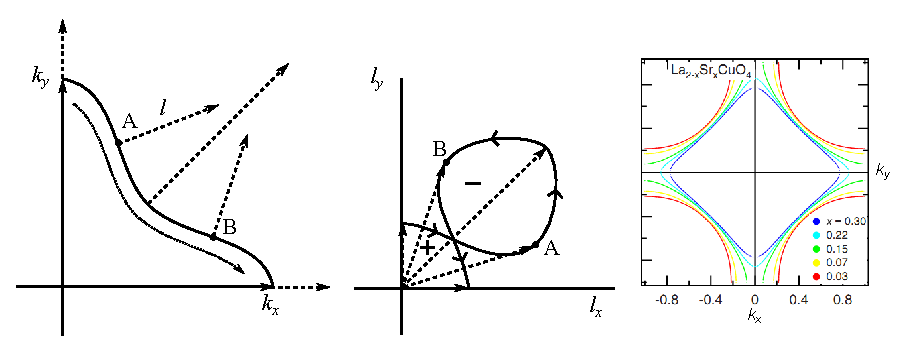
\includegraphics[scale=0.9]{Chapter-Theory/Figures/NegativeCurvatureLSCO/NegativeCurvatureLSCO}
        \caption{Left illustrates a negatively curved Fermi surface with a long mean free path along the $k = (\pi, \pi)$ portion and the integral progressing along the dotted line. Middle shows how the mean free path vector changes along the integral line tracing two loops of opposite direction. Adapted from ref.~\cite{Narduzzo2008}. Right shows the progression of the \ac{BSCO} Fermi surface about the van-Hove singularity. Adapted from ref.~\cite{Kondo2004}.}
        \label{Fig:Theo:NegativeCurvatureLSCO}
    \end{center}
\end{figure}
Narduzzo \etal{} argues that this illustrated scenario is close to what we find in \ac{LSCO} at high doping. Here the mean free path is affected by the anisotropic scattering rate detailed in the introduction section and the proximity of the van-Hove singularity leads to negative curvature in the long flat sides of the Fermi surface as it changes between hole-like and electron-like, as shown for \ac{BSCO} in the right side panel of figure~\ref{Fig:Theo:NegativeCurvatureLSCO}, adapted from ref~\cite{Kondo2004}.

The form of the equations set out originally by Ong~\cite{Ong1991} for a 2D metal derives a relation for the transverse conductivity, $\sigma_{xy}$ from the Boltzmann model are as follows,
\begin{equation}
    \sigma_{xy} = \frac{e^2}{h}\frac{2\phi}{\phi_0} \hspace{8px}\textrm{where}\hspace{8px}\phi = A_l B
\end{equation}
where $A_l$ is the `Stokes' area traced in the centre panel of figure~\ref{Fig:Theo:NegativeCurvatureLSCO} and $\phi$ is the flux through the Stokes area and $\phi_0 = h/e$ is the flux quantum. The Hall coefficient $R_H$ is given by,
\begin{equation}
    R_H = \frac{\sigma_{xy}}{\sigma_{xx}\sigma_{yy}}
\end{equation}
where, assuming symmetric scattering along the $x$ and $y$ directions of the conductivity tensor then,
\begin{equation}
    \sigma_{xx} = \sigma_{yy} = \frac{e^2}{4\pi^2 \hbar} \int^{2\pi}_0 k_F(\theta) l(\theta) d\theta
\end{equation} 
Contributions from isotropic scattering which affect $\sigma_{xy}$ are cancelled in $R_H$, however anisotropic scattering at regions of Fermi surface of particular curvature do contribute to the Hall coefficient.



\section{Magnetoresistance}

\subsection{Fermi liquid theory}




\chapter{Experimental Technique}

\begin{chapterabstract}
This chapter begins with descriptions of how the \ac{dHvA} measurements were performed, the equipment used and the analysis. Next, a description of the methods and code used to calculate susceptibility is supplied and finally descriptions of the magnetotransport measurements and analysis are detailed.
\end{chapterabstract}


\section{De Haas-van Alphen torque measurement}

In this section the measurement of \ac{dHvA} oscillations by the torque method is described. For decades, the measurement of \ac{dHvA} oscillations provided the principle method of characterising the Fermiology of a material with only relatively recent competition from techniques such as positron annihilation and \ac{ARPES} in particular. Whilst \ac{ARPES} can provide direct maps of Fermi surfaces within the \ac{BZ}, \ac{dHvA} has some advantages such as the fact that it is insensitive to surface effects such as crystal reconstruction, can determine cross-sectional areas with a relatively high resolution and also provides useful secondary measurements such as effective masses of the quasiparticle carriers.  Some disadvantages of the technique include the fact that \ac{dHvA} cannot locate particular cross-sectional orbits within the \ac{BZ} (thus relies on secondary knowledge such as \ac{DFT} calculations) and also that the high magnetic fields could potentially affect the Fermi surface, for example by splitting the energy levels. Regardless \ac{dHvA} continues to be a reliable technique for Fermi surface characterisation.

\subsection{Experimental apparatus}

Much of the experiment apparatus has already been described in great detail by Dr. C. Andrew in her thesis~\cite{Andrew2010}. Here we recap and also detail the points of difference. 
%Moreover, although important experimental parameters will be specified, full details of the configuration of the hardware is listed in appendix~\ref{Appendix:dHvAHardwareSetup}.

\subsubsection{Torque cantilever}

A highly sensitive measure of torque is required to pick up the moments experienced by the sample due to the field. For this reason a commercial piezoelectric \ac{AFM} cantilever, provided by Seiko corps., was repurposed to measure this. The sample was placed onto the topside of the lever above the \ac{AFM} tip. Previously this would be epoxied in place but for these measurements we tried successfully with using vacuum grease which freezes the sample in place at low temperatures. This has the added benefit of still being adjustable and removable when warmed back to room temperature. Moreover, when it comes to rotate the sample in the basal plane, this was possible by nudging the sample gently without having to move the cantilever and risk breaking the lever with the sample permanently affixed. Care should be taken not to get grease on the pivot point of the levers since this will freeze the lever in place at low temperatures.
\begin{figure}[htbp]
    \begin{center}
        \includegraphics[scale=1.1]{Chapter-ExperimentalTechnique/Figures/CantileverSchematic/CantileverSchematic}
        \caption{Photo of the \BaFeP sample mounted on the measurement lever along with a schematic showing the full cantilever assembly. N.b. the \BaFeP crystals often cleave along the $[110]$ plane and so despite the apparent $45^\circ$ rotation, the sample is aligned such that the lever flexes in the $[100]$ plane.}
        \label{Fig:Exp:CantileverSchematic}
    \end{center}
\end{figure}
The cantilevers feature a second dummy lever alongside the principle lever where the sample was mounted. Instead of measuring the voltage across the principle lever alone, we measure the difference of the voltages between the two levers using a Wheatstone bridge which is balanced using two \unit{500}{\ohm} resistors. This enables some degree of correction due to vibrations and fluctuations in measurement current and also allow for correction of magnetoresistance effects within the levers. The circuit is balanced using a variable resistor and is zeroed as best as possible within the noise before each measurement run.

The voltage is supplied and measured using Stanford SR830 lock-in amplifier. The input supplied to the Wheatstone bridge first passes through a \unit{10}{\kilo\ohm} resistor with an excitation voltage of \unit{1}{\volt} unless otherwise stated. The output is first amplified using an EG\&G 5113 pre-amplifier with a gain of $\times1000$ with a band pass filter which was suitably set for the lock-in amplifier excitation frequency. All of the circuitry mentioned above, aside from the cantilevers and leads, is kept outside of the fridge at room temperature and is away from the field centre by approximately \unit{2-3}{\metre}.

\subsubsection{Sample stage}

The cantilever is mounted onto the sample stage which is a one axis Swedish rotator fabricated entirely from hysol. This is moved by an external stepper motor controlled by a computer. 

The angle of the stage in relation to the field is determined by one of two orthogonal pick-up coils mounted on the sample stage. A weak, oscillating magnetic field is generated by a coil which is wound concentrically around the inside of the main magnet coil. The AC coil induces a voltage in these orthogonal pick-up coils on the stage which is proportional to the sine of the angle they are at with respect to the field. The pick-up coil voltage is measured by a second Stanford SR830 lock-in amplifier after passing through a custom amplifier set to $\times100$. The lock-in amplifier also drives the oscillating field after passing a custom built current source. The modulating coil is designed to generate an oscillating field of a few tens of Gauss whilst the main coil is in persistent mode~\cite{Instruments1998}.

% An upper bound on the strength is $\sim$\unit{333}{\textrm{Gauss}} RMS, based on a typical measured voltage of \unit{2.2}{\milli\volt} after $\times100$ amplification measured across a coil of $\sim140$ turns with an average area of \unit{3.36}{\milli\metre\squared} per loop.

\subsubsection{Yellow Magnet}

Measurements of the oscillations were all performed in Bristol on the `Yellow Magnet' system which was built by Oxford and can nominally operate up to \unit{20.5}{\tesla} with use of the lambda plate, an additional cooling system for the magnet coil, although is more typically operated up to \unit{18}{\tesla}.
\begin{figure}[htbp]
    \begin{center}
        \includegraphics[scale=1.1]{Chapter-ExperimentalTechnique/Figures/SampleStageSchematic/SampleStageSchematic}
        \caption{A photo of the Swedish rotator sample stage with cantilever in place and protective cap removed.}
        \label{Fig:Exp:SampleStageSchematic}
    \end{center}
\end{figure}
The bulk of the cryostat sits in a bath of $^4$He which takes the temperature down to the helium boiling point of \unit{4.2}{\kelvin}, and then the sealed sample space is additionally immersed in $^3$He gas in a Heliox system. This system condenses the $^3$He gas at the base of the chamber and pumps on it using a charcoal sorb to lower the sample stage temperature to $\sim$\unit{0.3}{\kelvin} for several hours before it has to be re condensed. Figure~\ref{Fig:Exp:YellowFridge} demonstrates the condensing cycle.
\begin{figure}[htbp]
    \begin{center}
        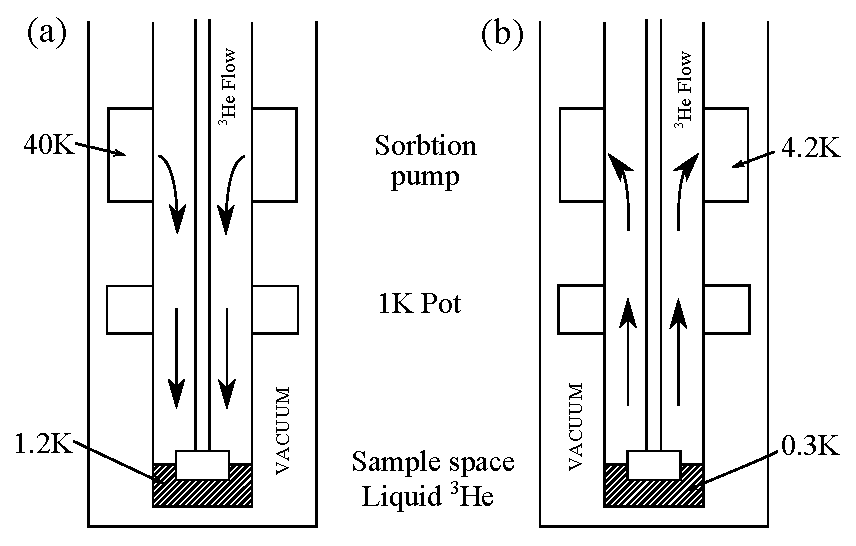
\includegraphics[scale=0.6]{Chapter-ExperimentalTechnique/Figures/YellowFridge/YellowFridge}
        \caption{The $^3$He condensing cycle for the Yellow Magnet Heliox. (a) The sorbtion pump is heated so the $^3$He it contains is released and condenses into a fluid on reaching the \unit{1}{\kelvin} pot. (b) Once a significant proportion of the $^3$He is condensed, then the pump heater is switched off which pumps on the liquid causing additional cooling around th esampel stage to $\sim\unit{0.3}{\kelvin}$}.
        \label{Fig:Exp:YellowFridge}
    \end{center}
\end{figure}
 In general measurements are taken at base temperature but higher temperatures can be achieved by heating the charcoal sorb pump thus lowering the pumping rate on the $^3$He bath. This technique allows access to temperatures up to approximately \unit{2.1}{\kelvin}. Temperatures greater than this are possible by heating the sample through an electric heater mounted on the magnet, however with our setup we do not accurately control temperature as the field ramps because of complications due to magnetoresistance effects in the measurement thermometers. Temperature is monitored at the sample by a Cernox thermometer on the sample stage, and a RuO$_2$ thermometer which is mounted in the sample space on the cryostat but is in thermal contact with the tip of the sample stage when the stage is properly seated. Care should be taken that this is the case to ensure effective pre-cooling of the sample. Further thermometers are situated on the \unit{1}{\kelvin} pot, the sorb and sat on top of the magnet coil although the latter is only monitored when initially cooling the magnet from room temperature. All thermometers and heaters were controlled using two Neocera LTC-21 temperature controllers.

Data is collected by a Windows PC running custom Delphi software which queues measurements and records data only. No analysis is performed in the collection software. Data is saved to text files.

\subsection{Data analysis}

\subsubsection{Angle correction}
    \label{Sec:Exp:AngleCorrection}

To perform angle dependent measurements, we need to first of all measure accurately the angle between subsequent measurements and second we need to determine the angle of the field compared to the basal planes of the crystal. 

In order to tackle the first problem, the pick-up coils sampling the AC field described earlier are used with the measured voltage begin proportional to the sine of the angle between the coil and the AC field. By monitoring this voltage, accurate determination of the angle between the sample platform and the field can be made and therefore the angle between subsequent measurements.

The absolute angle between the large DC field and the crystal planes in the sample were determined using a post-measurement correction. Since the frequency of the quantum oscillations are field dependent with turning points at the $B\parallel [001]$ direction for approximately two dimensional samples, an even termed polynomial up to fourth order was fitted to the peaks. From the minima of the fits an angular offset was obtained which gave the final correction to the above coil measurements.

The basal angle was aligned on the cantilever by eye. This was coupled with \ac{XRD} measurements which determined how the visual features corresponded to the crystal axes. This leads to an estimated error in basal plane alignment of around \unit{5}{\%} although we found evidence for greater misalignment in one case, detailed in the results.

\subsubsection{Temperature correction}
    \label{Sec:Exp:TemperatureCorrection}

Effective mass measurements on particular extremal orbits rely on accurate temperature determination at all stages of the field sweep. On the Yellow magnet system, temperature from base of $\sim$\unit{0.3}{\kelvin} to $\sim$\unit{2}{\kelvin} is controlled by adjusting the $^3$He sorbtion pump temperature and is largely independent of field effect since the thermometer regulating the sorb temperature is outside of the strong field core. However if we consider figure~\ref{Fig:Exp:TemperatureCorrection}, it is evident that there are magnetic field effects on the RuO$_2$, which is mounted in the base of the magnet but thermally linked with the sample, and the Cernox thermometer that sits on the sample stage.
\begin{figure}[htbp]
    \begin{center}
        \includegraphics[scale=0.9]{Chapter-ExperimentalTechnique/Figures/TemperatureCorrection/TemperatureCorrection}
        \caption{Some example temperature readings (filled symbols) set using the sorbtion pump heater. Also shown are corrections (open symbols) by interpolating to known values. RuO$_2$ thermometer is shown as circles, Cernox stage thermometer is shown as squares. Second order polynomial fits to the data are shown as lines extrapolated to zero to get a rough estimate of the zero field temperature value.}
        \label{Fig:Exp:TemperatureCorrection}
    \end{center}
\end{figure}
Readings from both thermometers were taken with field sweeps from zero field up to \unit{18}{\tesla} at steady temperatures \unit{0.30}{\kelvin}, \unit{0.53}{\kelvin}, \unit{0.64}{\kelvin}, \unit{1.06}{\kelvin} and \unit{1.34}{\kelvin}. By interpolating between this data\footnote{Performed using multiquadric radial basis functions from the Scipy Python library.}, the two thermometers can be corrected to agree within $\sim$\unit{0.01}{\kelvin}. This interpolation is however limited to temperatures below approximately \unit{1.45}{\kelvin} as is shown in the figure for readings at around \unit{1.6}{\kelvin}. In these cases, the less reliable method of extrapolating the readings back to zero field using a second order polynomial fit are used as demonstrated with the solid lines in figure~\ref{Fig:Exp:TemperatureCorrection}. In these cases the temperature is taken to be the mean of the two extrapolated values with the differences defining the error.

\subsubsection{Self heating effects}

The resistance across the piezo-electric lever is read by driving an AC current through it and reading the voltage across it using the Stanford lock-in amplifier. Larger currents are less prone to noise problems, however too much current results in self heating and subsequently the sample platform and sample could be at a higher temperature than the nearby thermometers suggest. To ensure that this is not the case we measure oscillations at constant temperature with a variety of driving currents. Small currents should not affect oscillation amplitudes, but at some current threshold self heating effects will become apparent and the oscillations are damped as if the entire system was operating at a higher temperature. We then resume measurements using a driving current below this threshold.

Ideally the temperature chosen should be on the steep part of the \ac{LK} temperature curve (eq.~\ref{Eqn:Theo:TemperatureTerm}) so that even small changes in temperature manifest in observable changes in the oscillation amplitude.

% \subsubsection{Field hysteresis correction}
% 
% Although the direction in which the field sweep occurs should not affect the oscillations, it was apparent that there was a slight shifting of the \ac{FFT} frequencies of the peaks in the down sweeps in comparison to the upsweeps. The shifts were larger at higher frequencies and generally would be of the order of \unit{0-40}{\tesla}. Since the effect was clear yet was of the order of the expected reolution at high fields, we simply applied a linear correction to the data set in order to bring the peaks into line. The corrections listed in table~\ref{Table:Exp:HysteresisCorrection} were either subtracted or added depending on the sweep direction.
% \begin{table}
%     \begin{center}
%            \caption{Correction factors linearly applied to the \ac{FFT} peaks due to hysteresis in the sweep direction.}
%         \begin{tabular}[htbp]{lll}
% \toprule
% Sweeps $B \to[110]$ & Corrn. at \unit{0}{\tesla}  & Corrn. at \unit{8000}{\tesla}\\
% \midrule
% $-31\degree$ to $-24\degree$  & 1 & 18 \\
% $-24\degree$ to $-13\degree$ & 9 & 20 \\
% $-13\degree$ to $100\degree$ & 1 & 21 \\
% \bottomrule
% & & \\
% \toprule
% Sweeps $B \to[100]$ & Corrn. at \unit{0}{\tesla}  & Corrn. at \unit{8000}{\tesla}\\
% \midrule
% $-31\degree$ to $100\degree$ & 3 & 13 \\
% \bottomrule
%         \label{Table:Exp:HysteresisCorrection}
%         \end{tabular}
%     \end{center}
% \end{table}

\subsubsection{Torque measurement factor}

An extra factor affecting the amplitude of the \ac{LK} oscillations occurs due solely to the nature of the torque oscillation measurement. The factor is given by,
\begin{equation}
    A_{\Gamma \textrm{(gen)}} = \frac{1}{F}\frac{dF}{d\theta_\perp}B
\end{equation}
where $\theta_\perp$ is the angle from the field direction. This can be simplified for a quasi $2d$ metal to,
\begin{equation}
    A_{\Gamma} = |\sin(\theta)|B
\end{equation}
where $\theta$ is the angle from the cylinder axis (usually in the $c$ direction). This means that at along the cylinder axis there will be no oscillations as $A_{\Gamma} \to 0$.


\subsubsection{Background removal}

Previous standard practice was to remove a background polynomial fitted to the field or inverse field from the raw data before taking the \ac{FFT}. With reference to figure~\ref{Fig:Exp:RawPlotAngleDependence}, raw torque data taken over a range of angles\footnote{See section\ref{Sec:ResD:AngleDependentMeasurements} for full details} and a strong $B^2$ component can be observed as a result of the $A_{\Gamma}$ term in the \ac{LK} equation at angles away from \unit{90}{\degree} and \unit{0}{\degree}. Figure~\ref{Fig:Exp:BackgroundSubtraction} shows in the centre and right panels that subtracting a second order polynomial fitted to the \emph{inverse} field leaves a large artificial angle-dependant oscillation in $1/B$ in the residual which may be misconstrued as a signal from a low frequency Fermi surface orbit, especially since there is an apparent angle dependence -- no such peak is seen for the flat curves at \unit{0}{\degree} and \unit{90}{\degree}. For this reason it is recommended to subtract a second order polynomial fitted to field rather than inverse field for torque measurements.
\begin{figure}[htbp]
    \begin{center}
        \includegraphics[scale=1.1]{Chapter-ExperimentalTechnique/Figures/ComparisonBackgroundSubtraction/RawPlotAngleDependence}
        \caption{The angle dependence of the raw torque data clearly showing a negative $B^2$ background at \unit{45}{\degree} and for $\theta<\unit{90}{\degree}$ and a positive $B^2$ background for $\theta>\unit{90}{\degree}$.}
        \label{Fig:Exp:RawPlotAngleDependence}
    \end{center}
\end{figure}
\begin{figure}[h!]
    \begin{center}
        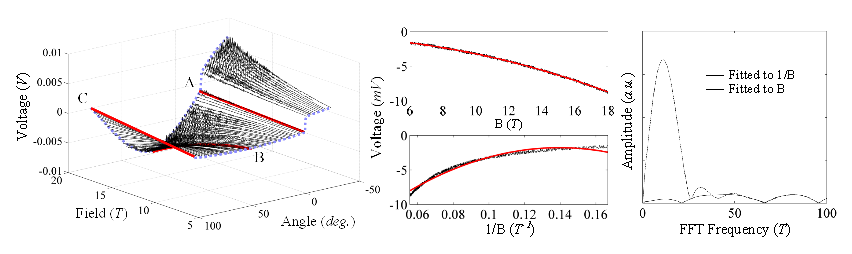
\includegraphics[scale=1.1]{Chapter-ExperimentalTechnique/Figures/ComparisonBackgroundSubtraction/ComparisonBackgroundSubtraction}
        \caption{Insets show a 2nd order polynomials fitted to simulated $B^2$ background with $\sim$\unit{0.5}{\milli\volt} of noise, similar in scale to that of \unit{45}{\degree} in figure~\ref{Fig:Exp:RawPlotAngleDependence}. Upper inset is fitted to field and lower to inverse field. The main figure shows the resulting \acp{FFT}.}
        \label{Fig:Exp:BackgroundSubtraction}
    \end{center}
\end{figure}

\subsection{Measuring the spin mass}
\label{Sec:Exp:MeasuringSpinMass}

Other than beating effect from similar frequencies, the only terms in the \ac{LK} equation that cause the amplitude to drop to zero as a function of angle are the torque term, $A_\Gamma$ which causes a single zero when the field is parallel with the cantilever arm and the spin term $A_S$\footnote{The angle dependence of $A_S$ comes from variations in the band mass}. By examining the amplitude as a function of angle it is possible to determine the spin effective mass. A good determination requires more than one spin zero (i.e. a non torque term zero) to be measured since the oscillatory nature of the $A_S$ term gives multiple solutions if we only have measured a single zero. We use $n$ to label each of the zeros from the $A_S$ oscillations.

% In practice the determination is complicated by the fact that if the Landau levels are very well defined, the double peaks due to Zeeman splitting do not overlap and so do not interfere. This manifests as a splitting of amplitudes which do not necessarily drop to zero. In these cases the zeros have to be best determined as being within the region where a noticeable increase in the number of spin split peaks occurs. Moreover, 

In practice, fitting the overall shape requires all of the \ac{LK} terms to be considered which makes free parameter fitting very difficult to converge. For these reasons, spin mass for this investigation is found from ansatz guesses for the values which are then fitted by inspection. Upper and lower bounds for the estimations are provided.

To the first approximation, the cylindrical approximation is used to describe the band mass in $A_S$, however the form of the spin term is relatively sensitive to small deviations and so fits would be much better using a more accurate variation of band mass with angle. Band mass was extracted from \ac{DFT} results and was performed using MATLAB code which locates the extremal areas from the corrected \ac{BZ} energy dispersion at a particular angle. Once located a small shift in energy is applied and the corresponding shift in area is used to determine the band mass using equation~\ref{Eqn:Theo:BandMass}. A polynomial of appropriate order is then fitted to the curve and used in the fitting routine in place of the band mass. The MATLAB code determines the masses with some spread in the values which caused higher order polynomial fits to oscillate at low angles within the noise. To alleviate this, a mean value was determined for each angle.

One final note is that the absolute value of the $A_S$ term is used to fit the data since we analyse the height of the \ac{FFT} peaks of the oscillations which are always positive and not the oscillations directly.

\subsection{Extracting effective mass from the temperature dependence}
\label{Sec:Exp:ExtractingEffMassTemperatureDependence}

Of all the damping terms in the \ac{LK} equation, only $A_T$ (eqn.~\ref{Eqn:Theo:TemperatureTerm}) is temperature dependent and so is used to determine the thermal effective mass. By measuring oscillations at a fixed angle but with varying temperatures, the effective mass can be determined in a number of ways.

\subsubsection{Basic \ac{LK} formula fitting}

The simplest technique to extract the thermal effective mass is to extract the amplitude of the oscillations from \acp{FFT} of the data at various $T$ and then perform a least squares fit to eqn.~\ref{Eqn:Theo:TemperatureTerm}. A particular problem with this approach is that it is not clear what value of $B$ should be used since the \acp{FFT} needs to span a field range when ostensibly the oscillation should be measured at a particular $B$ value. Generally the simplest thing to do is to take the \acp{FFT} over a small a range as possible and then take the field to be equal to the averaged inverse field\footnote{That is $B_{\textrm{av.}}^{-1} = \frac{1}{2}(B_{\textrm{min}}^{-1} + B_{\textrm{max}}^{-1})$}. 

There are two conflicting problems with this approach. First the amplitude tends to decreases with narrowing field range meaning weak oscillations may require larger field intervals. Secondly wider field ranges mean other attenuation factors --- which are also functions of $B$ --- affect the amplitude across the field sweep. The primary problem in this case is the Dingle term which has an exponential dependence on $B$. Although the Dingle term is not temperature dependent, the exponential dependence on the Dingle factor changes the amplitude of the oscillations over the field range necessary for the \ac{FFT} which can affect the final amplitude. Nonetheless, simple \ac{LK} fits are usually the first port of call and serve as a first approximation to the final result. For this investigation though, since we found some disagreement within the data, we employed a couple of additional techniques described below to overcome this shortcoming.

\subsubsection{Retrofitting ansatz \ac{LK} formulae}
\label{Sec:Exp:LKRetrofitting}

One of the primary field-dependant contributions to the oscillation amplitude is the Dingle term scattering (equation \ref{Eqn:Theo:DingleTerm}) which has an exponential dependence with temperature. The Dingle factor, $\alpha \equiv -\pi p m_b/e\tau$, can be determined by fitting a simplified version of the \ac{LK} equation,
\begin{equation}
    \Gamma_{\textrm{sim}} =  A_D(\alpha, B) \sqrt{B} \sin{\left(\frac{2\pi F}{B} + \phi \right)}
\end{equation}
 to oscillations which have been band pass filtered to reduce the number of contributions from other extremal orbits and hence the number of necessary fitting parameters. Once we have the Dingle term and also the peak frequency for a particular orbit, simulated oscillations are generated using the same equation but including the temperature term, $A_T(m^*_T, B)$, for a range of ansatz effective thermal masses. We then fit this to the \ac{LK} equation as described in the previous section. The mass that results from the fit is different from the actual effective mass used as the \ac{LK} fit has been affected by the Dingle term contribution. When we find a simulated oscillation that outputs the same effective thermal mass as the plain \ac{LK} fit on the actual data we then take the ansatz thermal mass for that matching fit to be the corrected thermal mass.

The filtering used to originally separate out the frequencies is band pass \ac{FFT} using a Hanning window.  This is adjusted in size and roll off width according to the peak. Occasionally, the peaks are too close together to effectively filter out individually and so two or three peaks were fitted at a time using a linear combination of the simplified equation above.

The initial fits were filtered using an existing Delphi program and fits to find $\alpha$ were performed in Kaleidagraph. Ansatz fits were found using a binary search technique using a Python script.


\subsubsection{`Microfitting' the \ac{LK} formula}
\label{Sec:Exp:LKMicrofitting}

A second technique is to filter out the individual orbit frequency by again using an \ac{FFT} filter and a Hanning window, and this time fitting small sections of sine curve ($\sim 1.5$--$3$ wavelengths) directly to the filtered torque data. This gives a field dependent value for the amplitude which can then be fitted to the standard $A_T$ form for many values of $B$. The result is a plot of mass values against $B$. Theoretically, these should plateau to give a constant value for the effective thermal mass.

Calculations were performed using a Python script to filter the data, perform the `microfits' and then perform the \ac{LK} fits. The script was tested using simulated data.





\section{Density Functional Theory}
\label{Sec:Exp:Dft}

Calculations presented in this thesis were performed using \WIEN version 07.2 (20th Feb 2007). Unless specified, non-spin orbit calculations are presented although spin-orbit calculations were checked and did not show significant differences. The \ac{GGA} according to Perdew-Burke-Ernzerhof was used for the exchange distribution.

Preprocessing of the WIEN2k data into voxel form as well as the theoretical angle plots were performed using a modified version of MATLAB code written by Dr. Ed Yelland. The basis for the code has been thoroughly field tested within the group over a number of years.


\section{Calculating susceptibility}
    \label{Sec:Exp:Susceptibility}

Code to calculate the Lindhard susceptibility was written in MATLAB \footnote{Full code is found in appendix~\ref{Sec:Appendix:SusceptibilityCode}.} and early versions were tested with free electron cases in 2 and 3 dimensions with results shown in figure~\ref{Fig:Exp:FreeElectronSusceptibility}. This matches the analytical results\footnote{See, for example, page 126 and Appendix F of ref.~\cite{Dressel2002}.}. One caveat when dealing with the free electron case is that the energy dispersion is not periodic and as such needs to be truncated at some point in a spherically symmetric way. This truncation affects the final calculation but provided it occurs far enough from the Fermi surface then the difference is minimal. The results shown are for a calculated region that was a sphere of radius 1 with a Fermi surface radius of 0.3. Values for $\delta$(=1e-9) and $\omega$(=1e-9) are somewhat arbitrary given that the dispersion is simplified with $\hbar^2/2m = 1$ but are given here for posterity. 

\begin{figure}[htbp]
    \begin{center}
        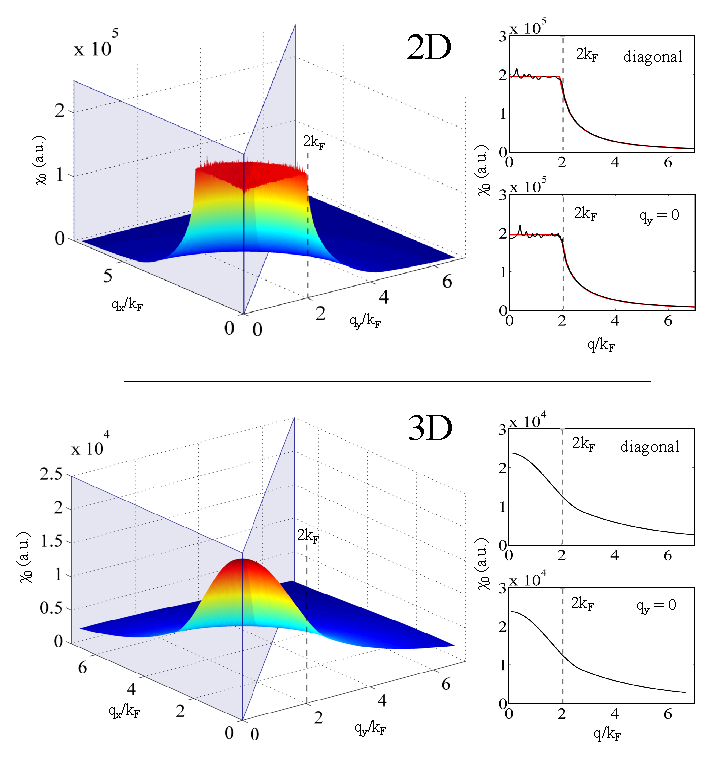
\includegraphics[scale=0.9]{Chapter-ExperimentalTechnique/Figures/Susceptibility/FreeElectron/FreeElectron}
        \caption{The real part of the Lindhard susceptibility calculations for a free electron model at \unit{T=0}{\kelvin} using the MATLAB \code{calc_x0.m} code. Top panels are for the 2D case over a $500\times500$ point grid, the bottom panels are for the 3D case taken over a $100\times100\times100$ point grid. Panels to the right correspond to slices through the surface plots on the left with red lines corresponding to the analytical form found in ref.~\cite{Blundell2001}. Calculations in the 3D case are at $q_z=0$.}
        \label{Fig:Exp:FreeElectronSusceptibility}
    \end{center}
\end{figure}


The code was adapted to accept pre-generated energy dispersions as calculated with the WIEN2k DFT software and post-processed with MATLAB code. In this case, the dispersion is periodic and energies at the scattering vector $q$ are obtained by simply `rolling' the 3D matrix of energy values. Testing on this adapted code was performed by re-creating WIEN2k calculations on LaFeAsO$_{0.1}$F$_{0.9}$ performed by Mazin \etal~\cite{Mazin2008} and then comparing our own susceptibility calculations with those in the Mazin paper. A temperature smearing of \unit{1}{\milli\textrm{Ry}} was quoted which equates to a temperature of \unit{157.88}{\kelvin}. A similar number of points ($55\times55\times26$) were also used.

Figure~\ref{Fig:Exp:MazinX0Comparison} show comparisons of $\Real \chi_0(q,\omega)$ and $\Imag \chi_0(q,\omega)$ with the published results. For these calculations the values of $\delta=\textrm{1e-4}$ and $\omega=\textrm{1e-6}$ were determined to give the closest results from a series of trials\footnote{There is no indication in the paper as to the values of $\delta$ and $\omega$ used in their own calculations although we know that they are likely to be of the order of the temperature energy scale (\unit{1}{\milli Ry}) or less.}. The comparison shows that some of the finer structure from the Mazin paper is missing from our own calculations, for example the depression in the real part at the $\Gamma$ point, however the overall shape is very similar.

\begin{figure}[htbp]
    \begin{center}
        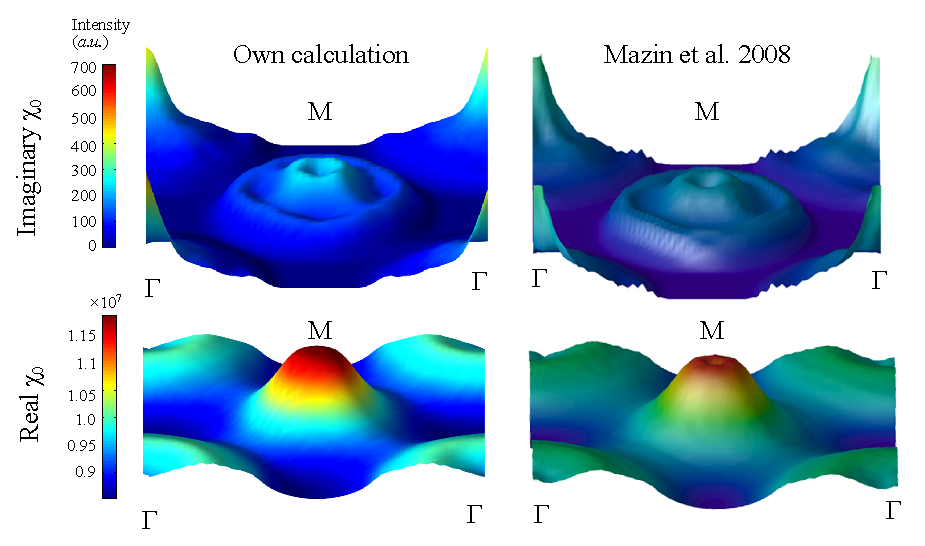
\includegraphics[scale=0.9]{Chapter-ExperimentalTechnique/Figures/Susceptibility/MazinComparison/MazinComparison}
        \caption{Right hand panels show the real and imaginary parts of Lindhard susceptibility calculations on LaFeAsO$_{0.1}$F$_{0.9}$ by Mazin \etal{} for $q_z=\pi/c$, right panels show the same calculation performed using our own MATLAB code.}
        \label{Fig:Exp:MazinX0Comparison}
    \end{center}
\end{figure}


The Lindhard function is very sensitive to details close to the Fermi surface and finite sampling of the energy data  can cause imperfect cancellation in the calculation --- particularly in the imaginary part. Applying a temperature smearing to the function is useful to gloss over the finite element size in the calculation which can cause significant spikes in the results. Figure~\ref{Fig:Exp:SusceptibilityTempSmearing} shows the smearing at a series of temperatures and that a temperature of \unit{158}{\kelvin} corresponds approximately to a smearing over 2 grid intervals at the Fermi surface. An appropriate choice of temperature depends on the granularity of the model as well as the expected fine detail of the results. The Mazin investigation was into a similar quasi two-dimensional pnictide material that used a comparable number of data points and so we also opted to use \unit{158}{\kelvin} for the temperature smearing.

Smearing also occurs when a finite quasi-particle lifetime, $\delta$, is factored in and when the perturbing field is oscillatory with frequency, $\omega$. These values are also not known a priori and so we again look to the energy scale of the spacing between grid points close to the Fermi surface for guidance.

\begin{figure}[htbp]
    \begin{center}
        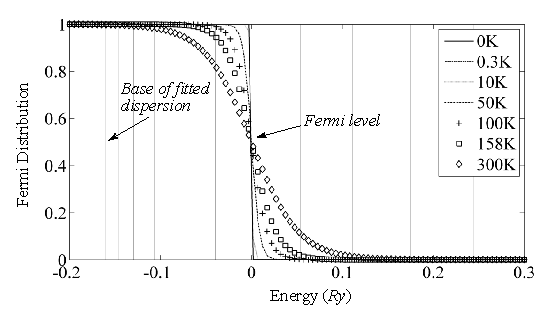
\includegraphics[scale=0.9]{Chapter-ExperimentalTechnique/Figures/Susceptibility/TempSmearing/TempSmearing}
        \caption{The Fermi distribution plotted at various temperatures. Vertical lines represent typical grid energy spacings for a free electron distribution fitted to a portion of bandstructure for LaFeAsO$_{01}$F$_{0.9}$ which rounds out just below the Fermi surface. We can see that for \unit{158}{\kelvin}, the smearing spans approximately 2 grid intervals at the Fermi energy.}
        \label{Fig:Exp:SusceptibilityTempSmearing}
    \end{center}
\end{figure}




\section{Measuring charge transport}

In this section the Hall measurement technique and analysis of the \ac{BSCO} samples is described. Transport measurements on superconductors have been performed for over a century now and was the technique by which superconductivity was first discovered. The relative technical simplicity of the measurements makes transport measurements highly appealing considering the wealth of information that can be extracted from a resistance curve.

The charge transport measurements performed for this thesis took place in Bristol in the Green `Polo' magnet for low fields and in the \ac{LNCMI} pulsed field facility in Toulouse for the high field data. Also included is analysis of data taken by other group members\footnote{Dr. X. F. Xu, Dr. P. Rourke and I. Mouzoupoulou} at the \ac{HFML} in Nijmegen, Netherlands. The overarching six-probe measurement technique is used for all the transport measurements with differences chiefly in measurement geometry and apparatus.

\subsection{Experimental apparatus}

\subsubsection{Six probe technique}

For accurate measurement of voltage, and hence resistance, across a sample, two wires are not sufficient. The wires and contacts themselves have a resistance which is comparable or often larger than the resistance of the sample being measured. A solution to this problem is to instead supply the current for the voltage reading via one set of wires, and then take the voltage reading from another set meaning that a minimum of four wires and four contacts on the sample are required. To measure magnetoresistance we require the voltage wires to be placed upstream and downstream of the current contacts, to measure the Hall effect we require the wires to be placed transverse to the current. Moreover it is useful to be able to take two transport measurements on opposite sides of the sample so as to get an idea for the homogeneity of the sample and as well to provide some redundancy in case of breakage. Since the \ac{BSCO} samples that we studied were to have both measurements, six connection points were placed on each sample as shown in figure~\ref{Fig:Exp:BSCOSampleSchematic}.
\begin{figure}[htbp]
    \begin{center}
        \includegraphics[scale=1.1]{Chapter-ExperimentalTechnique/Figures/BSCOSampleSchematic/BSCOSampleSchematic}
        \caption{An example \ac{BSCO} crystal mounted on the quartz substrate. Voltage legs are labeled (a), (b), (c) and (d).}
        \label{Fig:Exp:BSCOSampleSchematic}
    \end{center}
\end{figure}
The connections were made with \unit{20}{\micro\metre} gold wire for the current and \unit{10}{\micro\metre} gold wire for the voltage leads and attached with DuPont 4929 conductive silver paint which dries at room temperature. As shown in the figure, the sample is raised from the quartz substrate so that when the temperature drops and the wires and sample thermally contract at low temperatures, there is some give so that the ensemble does not pull itself apart due to thermal contraction.

With the four voltage legs a variety of configurations can be achieved. Measuring across (a) and (b) is the magnetoresistance configuration, (a) and (c) is the Hall configuration. It is also possible to measure across (a) and (d) and provided the field is reversed from positive to negative, both the Hall and the magnetoresistance across the sample can be extracted.

Because the connections may not be exactly aligned and because the silver paint in practice tends to whet over the edge of the sample, magnetoresistance contributions may be found in the Hall configuration and vise-versa. For this reason it is generally advised to sweep both with a positive field to obtain $R_{\textrm{pos}}$ and a negative field to obtain $R_{\textrm{neg}}$ where $R$ is the resistance and separate the two out using the technique described in the analysis section.

Later as the samples has been measured many times and thermal cycling had caused the silver paint to become brittle, it was necessary to attach short, $\sim\unit{2}{\milli\metre}$, secondary gold wires to each of the contact pads using silver paint and then attach the probe flying leads to the end of these wires. When removing the samples from the probe, this allowed the joins to be immersed in solvent held in the tip of a pair of metal tweezers at a safe distance from the sample ensemble meaning the connection could be dissolved without flexing the contact pads unnecessarily. This was done for the later measurements in the Polo magnet where the minimisation of wire loops was not so important.

\subsubsection{Polo magnet}

The `Polo' magnet is a cryostat from Cryogenic Ltd. containing a \ac{VTI} refrigeration device that allows temperature from $\sim$\unit{1.4}{\kelvin} to room temperature to be achieved. The \ac{VTI} system is a vacuum sealed chamber in to which the sample probe is inserted and sealed at the top. This chamber is insulated from a bath of $^4$He in the main cryostat by a vacuum jacket. $^4$He is admitted into the \ac{VTI} chamber from the bath via an adjustable needle valve and is pumped through the chamber and over the sample by an external roughing pump. By almost closing off the needle valve entirely and applying a heater on the sample stage the full range of temperatures can be achieved. In practice, a couple of temperature ranges are defined which require different operational techniques and are specified in table~\ref{Table:Exp:PoloOperation}.
\begin{table}
    \begin{center}
           \caption{Operating the \ac{VTI} under various temperature regimes.}
        \begin{tabular}[htbp]{lp{7cm}}
\toprule
Temperature range & Practice \\
\midrule
\unit{1.4}{\kelvin} -- \unit{4.2}{\kelvin} & Fill \ac{VTI} chamber with helium, close off needle valve and adjust the pumping rate to tune the temperature. \\
\unit{4.2}{\kelvin} -- \unit{300}{\kelvin} & Empty the \ac{VTI} of helium and open the needle valve slightly, only pump a small amount and use the sample heater to set the temperature.  \\
\bottomrule
        \label{Table:Exp:PoloOperation}
        \end{tabular}
    \end{center}
\end{table}
The \ac{VTI} chamber itself has an electric heater which can be operated separately and is good for rapidly heating the system up to room temperature but is in general too coarse for measurements.

Heating is controlled by a Lakeshore 340 temperature controller with the sample stage heated from the heater output and the \ac{VTI} heater controlled from the analogue output which has been boosted via a custom built amplifier unit. Sample temperature is monitored by a Cernox mounted onto the sample stage and \ac{VTI} temperature from a thermometer mounted inside the \ac{VTI} chamber.

The sample stage can be rotated by an external stepper motor which is supplied from a custom power source. All the instruments mentioned are controlled from a custom PC running a Delphi program written by Dr. M. French which queues runs, records and displays data. Some calculated values based on the raw data values are generated by the software, however these were not configured with the appropriate inputs. For this reason the angle and the current fields should be ignored and instead determined from raw data.

For twin voltage measurements, two Stanford SR830 lock-in amplifiers were used with one supplying the current and measuring voltage and the second synchronised to the first and also measuring a voltage. The current supplied was supplied through a \unit{1}{\kilo\ohm} buffer resistor in order to approximate the supply to a current source\footnote{i.e. if ($R_{\textrm{sample}} + R_{\textrm{wires}}) << R_{\textrm{buffer}} $ at all $T$, then the current is given by $V_{\textrm{excitation}}/R_{\textrm{buffer}}$.}. The resulting voltages were passed through two passive Princeton Applied Research model 1900 low noise amplifiers set to $\times1000$ before measurement although the actual amplification for typical resistances of $10$--$100\Omega$ at \unit{33}{\hertz} is $\times 980$.

The sample probe has a rotating stage and so after aligning the sample roughly by eye, a shallow angle sweep in a low field, typically \unit{1}{\tesla}, was performed before each measurement to make sure the sample was positioned perpendicular to the field. Some samples have an anisotropy in the transport terms and in the case of the Hall component, the effective field drops with the cosine of the angle of misalignment.

The magnet is superconducting and has a limit of \unit{14}{\tesla} or \unit{16}{\tesla} when using the additional cooling of the Lambda plate. For this thesis the measurements were only taken to \unit{13}{\tesla} to minimise the risk of a quench. The field was ramped at \unit{1.4}{\tesla\per\minute}. The measurements presented in this thesis from the Polo magnet are all taken in the Hall configuration and are obtained by averaging both sets of contacts as described in the analysis section.

As of Feb 2012 it was determined using a Cu sample that a positive reading of the magnet power supply current (and field) with the leads wired up correctly (i.e. positive to positive, negative to negative) corresponds to the magnetic field, $B$, in the Polo magnet pointing upwards. This was verified with a magnetic compass.


\subsubsection{\ac{HFML} Nijmegen}

To access the normal state of the higher $T_c$ materials we require fields larger than the \unit{13}{\tesla} available in the Polo magnet at Bristol. The \ac{HFML} facility in Nijmegen has available a continuous field Bitter magnet which can reach \unit{33}{\tesla}. Data from Nijmegen in this thesis was taken in May 2010 by Dr. X. Xu, I. Mouzoupoulou, Dr. P. Rourke and Dr. A. McCollam.

The magnet used at the \ac{HFML} sweeps at a rate of typically \unit{3}{\tesla\per\minute} meaning the temperature can drift significantly. The necessary heating supply for temperature control was alternated between a Lakeshore 340 temperature controller which uses input from a Cernox thermometer and a PID algorithm to supply an appropriate current or a Keithley current source which supplies a fixed current. The current source was selected on a sweep-by-sweep basis depending on which gave more stable temperatures.  The analysis compensates for small drift using a simple correction described later. 

The samples were measured using Stanford SR830 lock-in amplifiers which were supplying via \unit{1}{\kilo\ohm} resistors with a \unit{10}{\ohm} shunt resistor. A \unit{1}{\volt} excitation voltage was used for all samples except for B00KOD1a and B16KOD1a where \unit{2}{\volt} excitation was used instead. The excitation frequency is set to one of the `magic' frequencies\footnote{Frequencies that do not fall near common sources of noise or their harmonics e.g. \unit{50}{\hertz} from mains supply} which in this case were \unit{33}{\hertz}, \unit{77}{\hertz}, \unit{113}{\hertz} and \unit{123}{\hertz}.

Field is monitored using a calibrated Hall sensor mounted on the probe which is measured using another Stanford SR830 lock-in amplifier.

\subsubsection{\ac{LNCMI} Toulouse}

To obtain the highest fields we took measurements at the \ac{LNCMI} pulsed field facility in Toulouse over the course of two separate visits. Here large capacitor banks are discharged through liquid nitrogen cooled copper resistive magnets to achieve short (few tens of microseconds) but strong fields of up to \unit{60}{\tesla}. Pulses at the stronger end of the scale have more potential for damaging the magnet and take longer to cool down before the next pulse can be taken and so careful consideration is required to the magnitude of pulse undertaken. Typically the cooling time is around 15 to 30 minutes. The field is measured using a calibrated pick-up coil. The first trip took place in June 2009 and involved B. Arnold, Dr. P. Rourke, Dr. B. Vignolle and Prof. C. Proust. the second trip occurred in February 2010 and involved Dr. P. Rourke, Dr. J. F. Mercure, Prof. N. Hussey, Dr. B. Vignolle and Prof. C. Proust.

The results are recorded using a pair of Stanford SR830 lock-in amplifiers after passing through an active INA103 pre-amplifier set to a gain of $\times200$. The raw signal for the pulse duration is recorded and the lock-in in algorithm is post-processed in software to avoid wasted pulses due to incorrect settings. The driving current is supplied by the lock-in amplifier and unless otherwise noted is \unit{5}{\volt} through a \unit{1}{\kilo\ohm} resistor giving a current source of \unit{5}{\milli\ampere}. The driving frequency is typically very high to sample the data over the relatively short pulse time and for these experiments is typically \unit{60}{\kilo\hertz}. The data is streamed via an optical link along glass fibres (so the chamber remain electrically isolated for safety during a pulse) to an external PC.

Cooling down to $\sim \unit{1.4}{\kelvin}$ is possible by pumping on the helium in the magnet bath. Higher temperatures could be achieved by pumping out the exchange gas and heating via a Lakeshore 340 temperature controller. Although pulses are very short lived, there is a risk of the rapidly changing field inducing a current in the leads and sample which cause heating of the sample during the pulse. For this reason great care is taken to minimise current loops by minimising the non-twisted portion of the wires leading to the sample. Furthermore, the sample is physically jolted by the high field which can adversely affect the data, for this reason, vacuum grease is carefully applied to the sample ensemble to reduce movement.

For the first Toulouse visit, the measurements were taken in the magnetoresistance configuration, the second Toulouse visit measured the samples in the diagonal configuration.

\subsection{Sample size determination}

The length and the width of the samples were determined from calibrated optical microscope screen captures. The depth was determined post transport measurements with the help of Dr. P. Heard using a \ac{FIB}. This images samples by rastering a focused beam of ions onto the sample surface and measuring the amount of ejected electrons or ions form the image. This process causes electrical charging of the surface which can in turn adversely affect the path of the highly focused incoming ions and so the sample to be imaged must be earthed in order to remain electrically neutral. For these samples, a line of 4929 silver paint was drawn between on of the contacts and the sample mounting puck.

\subsection{Data Analysis}

\subsubsection{Isolating Hall and \ac{MR} components}

When measuring transport in a sample, there will always be contributions from both the \ac{MR} and the Hall components due to imperfect geometry of the voltage pick up points. Since the Hall component reverses sign as the polarity of the field reverses whereas the \ac{MR} component is independent of field polarity, the Hall and \ac{MR} components can be separated out using the following relations,
\begin{align}
\label{Eqn:Exp:HallMRExtraction}
R_{\textrm{Hall}} &= \frac{1}{2}( R_{\textrm{pos}} - R_{\textrm{neg}} ) \\
R_{\textrm{MR}} &= \frac{1}{2}( R_{\textrm{pos}} + R_{\textrm{neg}} )
\end{align}
where $R_{\textrm{pos}}$ and $R_{\textrm{neg}}$ are the resistances measured for the positive and negative field polarities. This requires data to be taken from the positive field maximum down to the negative field maximum and so for example with the Toulouse pulsed field apparatus, two pulses are required for each measurement.

% \subsubsection{Analysis of the Hall angle}

% In metals the Hall component does not vary with temperature, however high-$T_c$ materials have consistently demonstrated a distinct non-trivial temperature dependence. One way to tackle this problem was pioneered by Chien \etal~\cite{Chien1991} who studied the Hall angle, $\cot\theta_H = \rho(T) / (R_H(T) B)$, of \ac{Y123} doped with Zn impurities and found it to follow $\cot\theta_H = a T^2 + C$ where $C$ is a constant term due to impurities. The Hall angle, $\tan^{-1}(\sigma_{xy}/\sigma_{xx})$, is thought to cancel contributions from the transport scattering rate leaving the only the transverse scattering rate and so provides a way to access the `actual' Hall contribution.


\subsubsection{Correcting for temperature variations}

Figure~\ref{Fig:Exp:ComparisonFieldSweeps} shows a comparison of typical field sweeps for the \ac{LNCMI} and Nijmegen facilities and the Polo magnet. The \ac{LNCMI} pulse length is $\sim\unit{150}{\milli\second}$ and as such is not typically subject to slow temperature drift throughout the duration of the pulse. However the positive and negative pulses are typically taken with at least a \unit{30}{\minute} interval in-between pulses meaning the positive and negative pulses may not be at precisely the same temperature. As such, a small offset is applied to bring the zero field data into line between positive and negative pulses.
\begin{figure}[htbp]
    \begin{center}
        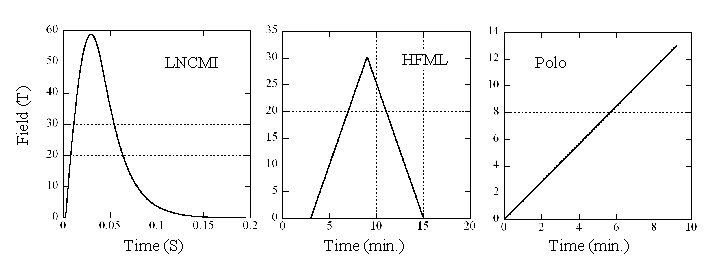
\includegraphics[scale=0.9]{Chapter-ExperimentalTechnique/Figures/ComparisonFieldSweeps/ComparisonFieldSweeps}
        \caption{From left to right: Typical field sweep profiles for a pulse at the \ac{LNCMI}, Toulouse, a continuous positive sweep at the \ac{HFML}, Nijmegen and single positive upsweep for the Polo magnet, Bristol}
        \label{Fig:Exp:ComparisonFieldSweeps}
    \end{center}
\end{figure}
For the longer sweeps such as the Nijmegen data sets, an additional offset was applied to the measurement which is proportional to the temperature as detailed below,
\begin{equation}
    R_{\textrm{corr.}} = R_{\textrm{meas.}} + F(T_{\textrm{base}} - T_{\textrm{meas.}})
\end{equation}
where $R_{\textrm{corr.}}$ is the corrected resistance, $R_{\textrm{meas.}}$ is the measured resistance, $T_{\textrm{base}}$ is the temperature that the temperature that the resistance values are converged towards and $F$ is an empirical scaling factor that brings the upsweep and downsweep data into line. The empirical factor was determined by inspection using the following method.
\begin{enumerate}
\item Take data where there is a clear component that is due to the temperature drift and find the appropriate factor so that it disappears. Take these data as reference benchmarks.
\item Where the temperature component is not so clear, use the reference data and make an informed estimate of the factor based on resistance vs. temperature curves in zero field and \unit{13}{\tesla}
\end{enumerate}
The same factor is applied to both the positive and negative sweeps to avoid introducing artificialities into the Hall gradient. For the Polo data the temperature control was such that no correction was necessary.

\subsubsection{Field lag correction}

The Polo magnet has no sensor to measure field at the sample, with the field values being calculated from the power supply current. In the data there is evident hysteresis in all sweeps and is illustrated in figure~\ref{Fig:Exp:PoloHysteresis} which suggests that the actual field lags slightly behind the indicated field possibly due to induction effects in the magnet coil and/or the power supply. To correct for this, the upsweeps and downsweeps were shifted towards each other until they overlapped, typically each by around \unit{0.2}{\tesla}. Any values which were corrected to less than \unit{0}{\tesla} or more than \unit{13}{\tesla} were then not used in the analysis.
\begin{figure}[htbp]
    \begin{center}
        \includegraphics[scale=1.1]{Chapter-ExperimentalTechnique/Figures/PoloHysteresis/PoloHysteresis}
        \caption{An example of the measured voltage of separate up and downsweeps which demonstrate the lag in actual field compared to the indicated field}
        \label{Fig:Exp:PoloHysteresis}
    \end{center}
\end{figure}

\subsubsection{Combining up and downsweeps}

For all the data values there is an upsweep portion and a downsweep portion which overlap and are averaged together to reduce noise. However many portions of data have regions which drift due to changes in the out-of-phase component or anomalies such as spikes and so in these cases the regions are recorded in a configuration file and the scripts that combine the sweeps ignore the problem regions and instead use data from the counterpart sweep in isolation. Similarly, when hysteresis is encountered in the pulsed data, by convention the upsweep is ignored since it is more rapid than the downsweep which generally results in more spikes and out of phase problems.

To obtain the Hall and \ac{MR} components using equation~\ref{Eqn:Exp:HallMRExtraction} we need to obtain comparable data points with shared field values. To do this one of two technique was employed. For the high-field data, this is done by binning the data and taking the average of the values in each of the bins so that they share the same field values. The data taken from the Polo magnet is linearly interpolated to a predefined set of field values.

\subsubsection{Linear fits to Hall data}

Hall data for all samples were fitted using a standard linear least squares fit which was performed using Python for the Polo data and Delphi for the high-field data due to the different preprocessing requirements described in the previous section. A cutoff is specified so that only the data above the cutoff is fitted in the region where the linear behaviour is recovered. The cutoff value is found by inspection of the Hall data with reference to the \ac{MR} component. The precise point where linear behaviour is recovered is not always clear and so two cutoffs were specified which defined the upper and lower bounds for the start of the linear region. The limits contribute to the error in the Hall gradient with the final gradient being taken as the average of the fits from the two cutoff limits.

\subsubsection{Normalising the high field data}

The Polo data was taken in the Hall configuration and so corresponds to the true Hall voltage, whereas the data from the first visit to the \ac{LNCMI} was on sample measured in the \ac{MR} configuration and so represent some unknown fraction of the true Hall voltage. Moreover, the rest of the high field data was taken in the diagonal configuration meaning the voltage path was over a different portion of the sample to the Hall measurement which again means the Hall voltage is scaled by some factor. For these reasons the Polo magnet measurements were taken as the canonical absolute values for the Hall data, with the high field data scaled so that concurrent data at higher fields aligned, this process along with the variation between fits using the two different cutoff bounds define the error bars in the data.


\subsection{Determining the doping}

Three techniques have been identified for determining the doping for this thesis. The most simple and well known method for determining the doping of a material utilises the so-called `universal' Tallon relation~\cite{Presland1991} which links $T_c/T_c(\textrm{max})$ to $p$ as follows,
\begin{equation}
\label{Eqn:ExpH:TallonRelation}
T_c/T_c(\textrm{max}) = 1 - 82.6 (p - 0.16)^2
\end{equation}
This relation was established based on measurements of \acf{LSCO} which exploit the direct relation between Sr content and the doping (assuming stoichiometric oxygen).

The second technique, particular to \ac{BSCO}, was published by Ando \etal~\cite{Ando2000} in 2000 where samples of \ac{BSCO} were compared with Hall measurements of other cuprates where the carrier concentration is more easily determined, in particular \ac{LSCO} was used again. The results lead to a very different relation between $T_c/T_c{\textrm{max}}$ which confined superconducting samples to a much narrower range of dopings\footnote{The justification being that increasing disorder suppressed $T_c$ as you move away from optimal doping} and is given by the following relation,
\begin{equation}
\label{Eqn:Exp:AndoRelation}
T_c/T_c(\textrm{max}) = 1 - 254.3 (p - 0.16)^2
\end{equation}
which was extracted from the Ando paper based on dopings determined by La concentrations. 

There is however some doubt as to whether it is appropriate to compare \ac{LSCO} and \ac{BSCO} measurements across the superconducting dome, especially with regards to Hall measurements, given the proximity of the van-Hove singularity in \ac{LSCO} which should lead to a depression in the apparent carrier density above $p=0.18$.

The final technique is by comparing instead \ac{BSCO} and \ac{TL2201} which have very similar structures, and van-Hove singularities at much higher doping than \ac{LSCO}\footnote{\ac{TL2201} has a van-Hove singularity at a much higher doping than even \ac{BSCO}. At $p=0.26$ (or rather $p=1.26$), \ac{ARPES} measurements have shown the van-Hove singularity in \ac{TL2201} lies a few \unit{eV} below the Fermi energy~\cite{Plate2005}} . Doping in \ac{TL2201} has been well characterised in the overdoped side through recent \ac{dHvA} experiments~\cite{Bangura2010} which maps well to where the majority of our \ac{BSCO} samples lie. Here the doping is determined using the Tallon relation for underdoped to slightly overdoped samples with $T_c/T_c(\textrm{max})$ down to $0.71$, below this value a linear relation is used: $T_c/T_c(\textrm{max}) = 2.390 - 7.696p$. Again some a priori knowledge of the approximate location (i.e. overdoped or underdoped) on the superconducting dome is required and further investigation may be required to determine which side of the dome a sample lies.




\chapter{dHvA measurements on \BaFeP}


\section{The \BaFePAs series}

The \BaFePAs series is one of many that stem from the parent compount \BaFeAs, although unlike the electron doped \BaCoFeAs and the hole doped \BaKFeAs series, the \BaFePAs progression is entirely isovalent meaning that the changes affected due to the P substitution are due to structure and chemical pressure rather than additional charge carriers. Nonetheless, superconductivity occurs with a very similar phase diagram as with the charge-doped examples in the same `$122$' family of iron-pnictide materials.\footnote{See for example \Fig1 in ref.\cite{Paglione2010}}

At $x=0$ the \BaFePAs series begins at \BaFeAs, a compound which becomes antiferromagnetic at around \unit[138]{K}, and moves with increasing $x$ towards \BaFeP which is metallic to low temperatures. Neither end members are superconducting, however as As is substituted for P, the low temperature antiferromagnetic state decays, giving way to superconductivity which kicks in at approximately $x=0.18$ and increases to the optimal substitution of $x=0.31$. Superconductivity then decreases until it gives way to a paramagnetic ground state at around $x=0.71$. \Fig\ref{Fig:ResD:PhaseDiagram} shows the phase diagram adapated from ref. \cite{Nakai2010a} as determined by resistivity measurements. 
\begin{figure}[htbp]
    \begin{center}
        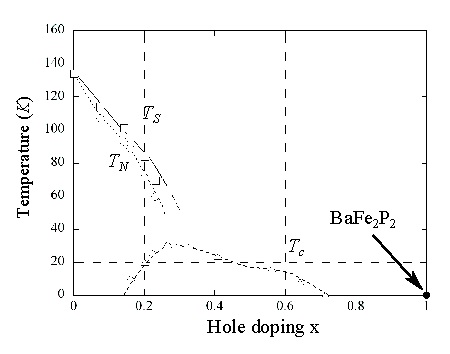
\includegraphics[scale=1.0]{Chapter-dHvABaFe2P2/Figures/BaFe2P2Series/PhaseDiagram/PhaseDiagram}
        \caption{Phase diagram adapted from ref \cite{Nakai2010a} measured by resistivity. $T_s$, $T_N$ and $T_c$ are the structural transition, the antiferromagnetic transition and the superconducting transition temperatures respectively.}
        \label{Fig:ResD:PhaseDiagram}
    \end{center}
\end{figure}
Also detailed in the phase diagram is the structural transition which occurs as the tetragonal $I4/mmm$ cell moves to an orthorhombic cell as it passes below the line marked $T_s$. This is a feature which is common to many of the `$122$' pnictide materials.

 The progression along the series is isovalent since P and As are in the same periodic group -- group $V$. The net effect of the substitution is to apply an increasing chemical pressure as $x$ moves towards $1$. Several reports show that applying \textit{physical} pressure to \BaFeAs results in a similar phase diagram with an antiferromagnetic phase and superconductivity up to $\sim$\unit[30]{K}\cite{Yamazaki2010,Colombier2009,Alireza2009} with Klintberg \textit{et al.}\cite{Klintberg2010} presenting a direct comparison between the two types of pressure. As pressure is applied, the unit cell $a$ axis shrinks slightly less than the $c$ axis ($\sim3\%$ c.f. $\sim4.5\%$ respectively). Interestingly the $c$ axis shrinking largely occurs in the Fe-Pnictide plane leading to some theories of the superconductivity emerging from the tetrahedral bond angle between the Fe and the pnictigen. %TODO: ref read Kuroki
\begin{figure}[htbp]
    \begin{center}
        \includegraphics[scale=1.0]{Chapter-dHvABaFe2P2/Figures/BaFe2P2Series/UnitCell/UnitCell}
        \caption{The tetragonal unit cell of the 122 \BaFePAs series.}
        \label{Fig:ResD:UnitCell}
    \end{center}
\end{figure}


The \BaFePAs series from a substitution of $x=0.41$--$1.0$ has been previously measured by members of the group at Bristol using dHvA oscillations\cite{Shishido2010}. As suggested in the Shishido reference, since dHvA has been observed across such a large range of substitutions, it implies that the material is not prone to disorder as is the case in many charge doped series (TODO ref) making the series an excellant candidate for dHvA studies. The Fermi surfaces have been characterised for x ranging from $0.41$ to $1$ for electron sheets only but have clearly shown that the DFT calculations consistently overestimate the size of the surfaces. Moreover, dHvA measurements on the material with $x=0.63$ have been performed where one of the hole surface extrema was observed\cite{Analytis2010c} however DFT calculations as well as comparisons with \SrFeP\cite{Analytis2009} give evidence for a second hole Fermi surface for materials towards the P end of the series, (towards the As end of the series, there appears this second hole and a \textit{third} hole surface similar but smaller to the other hole sheets). If the electron Fermi surfaces are oversized in the DFT calculations, then the hole Fermi surface volumes should also be oversized in order to remain compensated (electrically neutral). What is not clear though is whether the \textit{shapes} of the hole pockets are also altered in the compounds leading to \BaFeP. DFT calculations show the larger of the hole pockets in particular undergoing significant geometric changes, specifically in that it becomes much more three dimensional as P substitution becomes more complete. The Fermi surface of the opposite end-member, \BaFeAs, has been fully characterised by previous ARPES measurements\cite{Kondo2010a} and dHvA\cite{Terashima2011, Analytis2010b}. Coupled with a full characterisation of the fermiology of \BaFeP, this data can be used to interpolate Fermiology of the hole pockets between end members thus completing the partial determination of the Fermi surfaces of the intermediary compounds.

The ARPES measurements of the Fermi surface of \BaFeAs below the N\'eel temperature concluded that despite some $k_z$ dispersion in the Fermi surfaces, there is adequate nesting to form the antiferromagnetic state. Ab-initio DFT calculations\cite{Shishido2010} of the paramagnetic state have shown the $k_z$ dispersion increasing with increasing P, with the outer hole pockets becoming more three-dimensional through the progression providing the partial nesting conditions necessary for pair forming SDW fluctuations described in section\ref{Sec:1:Nesting}. One caveat is that these calculations do not take into account the structural changes below $T_s$, another caveat is that they do not consider Fermi surface reconstruction due to the observed commensurate antiferromagnetic order. To fully settle the issue of the nature of the nesting in the superconducting state, experimental determination of the Fermi surfaces of the series is necessary, a good guide to which can be obtained from study of the end-members.


This thesis presents data which details the full Fermi surface of \BaFeP including an elucidation of the shape of the 3D outer hole surface. Partial nesting is detailed between the outer hole surface and the inner electron surface with $q=(\pi, \pi, \pi/2)$ meaning the phenomenum persists through to the end member of the series. Also presented are effective mass measurements which show relatively small mass enhancements implying weak carrier correlations.



\section{X-Ray Diffraction}
    \label{Sec:ResD:XrayDiffraction}

The crystalline axes of the sample were determined by \ac{XRD} on a Kappa Apex II single crystal diffractometer with the aid of Dr. M. Haddow. The sample was mounted on a glass rod and held in place using vacuum grease. Clear diffraction spots are visible on the example scans shown in figure~\ref{Fig:ResD:XRayDiffraction} although there is some evidence of a second, misaligned phase with the doubling of the spots in a small number of the scans such as the one in the top left panel. There is also further evidence of secondary phases as some peaks are doubled up in the dHvA data presented later. We have no reason to believe however that these speculated misalignments are significantly affecting the rest of the body of results nor that they affect the conclusions in any appreciable way.

Perhaps surprisingly, the straight edge of the crystal was found to lie along the $[110]$ direction and not along the unit cell axis. This was found to be the case for a number of other \BaFeAsP{} crystals which were x-rayed later in the year.

\begin{figure}[htbp]
    \begin{center}
        \includegraphics[scale=0.7]{Chapter-dHvABaFe2P2/Figures/Xrays/XRayDiffraction/XRayDiffraction}
        \caption{Panels show example diffraction patterns of the \BaFeP{} sample. Left shows a zoomed portion of doubled peaks indicating that there may potentially be a misalignment within the crystal. Right inset shows the labelled crystal axes superimposed on the sample which is mounted on a glass rod.}
        \label{Fig:ResD:XRayDiffraction}
    \end{center}
\end{figure}

Lattice parameters are determined using the Apex II software and are presented in table~\ref{Table:ResD:LatticeParams} along with comparisons to two previous measurements found in the literature. The result agree within the error.
\begin{table}[htbp]
    \begin{center}
        \caption{Lattice parameters from \ac{XRD} measurements compared with literature.}
        \begin{tabular}{llll}
\toprule
Source  &  $a$ (\AA) & $c$ (\AA) & $z_P$ (\% $c$)\\
\midrule
X-ray   & $3.86(4)$  & $12.42(9)$ & \\
Rotter \etal~\cite{Rotter2010} & $3.8435(4) $ & $12.422(2)$ & $34.59(1)$ \\
Mewis \etal~\cite{Mewis1980} & $3.8400$ & $12.4420$ & $34.560$ \\
% Mewis \etal~\cite{Mewis1980} & $3.63$ & $11.76$ & $34.56$ \\
\bottomrule
        \label{Table:ResD:LatticeParams}
        \end{tabular}
    \end{center}
\end{table}



\section{Angle dependent measurements}
    \label{Sec:ResD:AngleDependentMeasurements}

\subsection{Determining experimental parameters}

Preliminary measurements showed very strong \ac{dHvA} oscillations which begin at relatively low field with an example of the raw data shown in figure~\ref{Fig:ResD:RawOscillations}. Since it is not clear from the raw torque data where the oscillations begin, Fourier transforms were taken with small (\unit{1}{\tesla}) field intervals --- the interval where a clear signal is present marks the onset of oscillations. An \ac{FFT} of the data for the ranges \unit{4-5}{\tesla}, \unit{5-6}{\tesla} and \unit{6-7}{\tesla} are shown in the insets of the figure. The range \unit{6-7}{\tesla} clearly shows the electron peaks at around \unit{1500}{\tesla} and \unit{2450}{\tesla}, with the higher frequency peak disappearing in the \unit{5-6}{\tesla} range and both peaks disappearing in the \unit{4-5}{\tesla} range. Further refinement suggests the onset of appreciable oscillations is around \unit{5.6}{\tesla} for the strongest electron peak. The field was ramped between \unit{6}{\tesla} and the safe maximum of \unit{18}{\tesla} for the vast majority of measurements bar some sweeps where the magnet was ramped to or from \unit{0}{\tesla} following or preceding shut-down of the magnet.

\begin{figure}[htbp]
    \begin{center}
        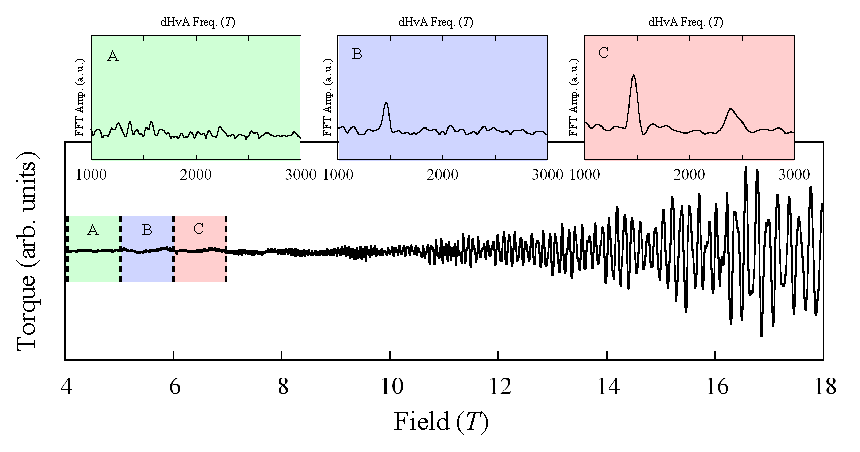
\includegraphics[scale=0.7]{Chapter-dHvABaFe2P2/Figures/AngleDepMeasurements/RawOscillations/RawOscillations}
        \caption{An example of the torque data taken with field aligned at \unit{26}{\degree} on the reverse side of the $[001]$ to $[100]$ angle sweep detailed later. Insets show a \acp{FFT} of the data between \unit{4-5}{\tesla}, \unit{5-6}{\tesla} and \unit{6-7}{\tesla} respectively. These intervals are marked on the main plot as A, B and C.}
        \label{Fig:ResD:RawOscillations}
    \end{center}
\end{figure}

Figure~\ref{Fig:ResD:ComparisonSweepRates} shows some example Fourier transforms of data taken at various field sweep rates and plotted with the frequencies shifted arbitrarily for ease of comparison. The difference in amplitude between the sweeps at \unit{0.05}{\tesla\reciprocal\minute} and \unit{0.1}{\tesla\reciprocal\minute} is less than \unit{1}{\%} whereas the difference when sweeping at \unit{0.2}{\tesla\reciprocal\minute} is nearly \unit{5}{\%}. Unless otherwise stated, subsequent sweeps were performed at \unit{0.15}{\tesla\reciprocal\minute} at the edge of where the sweep rate makes a significant difference in amplitude.

\begin{figure}[htbp]
    \begin{center}
        \includegraphics[scale=0.7]{Chapter-dHvABaFe2P2/Figures/AngleDepMeasurements/SweepRateComparison/SweepRateComparison}
        \caption{FFTs showing the peak from the smaller branch of band $3$ taken at, A: \unit{0.05}{\tesla\reciprocal\minute}, B: \unit{0.1}{\tesla\reciprocal\minute} and C: \unit{0.2}{\tesla\reciprocal\minute}. The peaks are arbitrarily shifted in frequency for ease of comparison. Measurements taken with $H$ at \unit{10}{\degree} from $[001]$ in the $[110]$ direction.}
        \label{Fig:ResD:ComparisonSweepRates}
    \end{center}
\end{figure}

In order to make a reasonable determination of the Fermi surface of a material, an appropriate number of angle sweeps need to be made to adequately constrain the shape of the Fermi surface. Since \BaFeP is a tetragonal system, any sweep from the azimuthal direction $[001]$ down the polar plane effectively expands to four due to the fourfold symmetry. Measurements were taken at one degree intervals from $H\parallel[001]$ down to $H\parallel[100]$ and from $H\parallel[001]$ down to $H\parallel[110]$ which, in this system, effectively amount to eight sweeps.

\begin{figure}[htbp]
    \begin{center}
        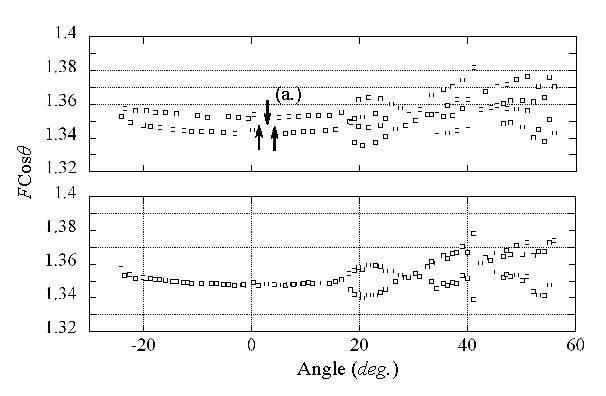
\includegraphics[scale=0.9]{Chapter-dHvABaFe2P2/Figures/AngleDepMeasurements/HysteresisCorrection/HysteresisCorrection}
        \caption{The plots show the $F\cos \theta$ for the $\alpha$ branch in the $[100]$ direction. Top panel shows the branch with the hysteresis due to field sweep direction, the bottom panel shows the data after the linear adjustment described in the main text. Arrows at point (a.) show how the points were shifted.}
        \label{Fig:ResD:HysteresisCorrection}
    \end{center}
\end{figure}

In general, runs were performed with an excitation voltage of \unit{1}{\volt}. To ensure that there was no self heating effects, runs were also performed with an excitations voltage of \unit{0.5}{\volt} and \unit{2}{\volt} at $T\approx$\unit{0.6}{\kelvin} (where we expect the \ac{LK} curve to be steep) and no change in oscillation amplitude due to heating was observed.

The magnetic field was alternatively ramped up and then down meaning subsequent measurements were generally performed with the magnetic field ramping in opposite directions. Although in theory this should not affect the results in any way, subsequent \ac{FFT} peaks appeared to alternately be shifted by up to $\sim\pm$\unit{21}{\tesla} with the magnitude of the shifts being roughly proportional to frequency. Assuming that the shifts were an artefact of the measurements, a linear correction determined by visual inspection was applied of $F_{\textrm{corr.}} = 3 + \frac{10}{8000} F_{\textrm{meas.}}$ for the sweep in the $[100]$ direction and $F_{\textrm{corr.}} = 0 + \frac{21}{8000}  F_{\textrm{meas.}}$ and  $F_{\textrm{corr.}} = 0 + \frac{18}{8000} F_{\textrm{meas.}}$ for the two sets of measurements performed to complete the sweep in the $[110]$ direction. Figure~\ref{Fig:ResD:HysteresisCorrection} shows an example of these hysteric shifts and the subsequent correction applied.

\begin{figure}[htbp]
    \begin{center}
        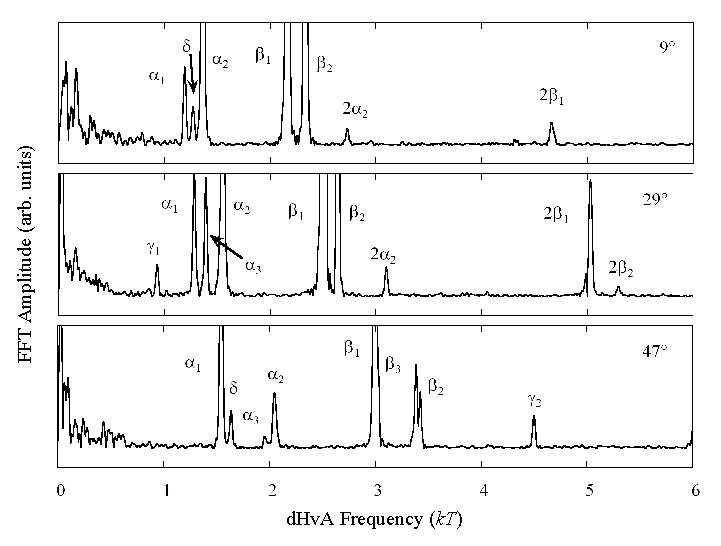
\includegraphics[scale=0.7]{Chapter-dHvABaFe2P2/Figures/AngleDepMeasurements/FFTExamples/FFTExamples}
        \caption{\ac{FFT} after a second order polynomial background was subtracted at various labelled angles between $[001]$ and $[110]$. The labels for peak identification are explained in the next section.}
        \label{Fig:ResD:FFTExamples}
    \end{center}
\end{figure}

Figure~\ref{Fig:ResD:FFTExamples} shows three example \acp{FFT} which show peaks from all the principal bands identified the next section. They also show first and second harmonics\footnote{Third harmonics were also identified in other \acp{FFT}, these are shown in figure~\ref{Fig:ResD:AngleSweepMeasured}.}. The low frequency region in figure~\ref{Fig:ResD:FFTExamples} shows noise from the cantilever, but according to \ac{DFT} fits performed in the next section, this region also likely contains signal from the minimum of band $1$. Given that the signal from electron bands is generally small due to high scattering rate, we were not able to extract a convincing Fourier peak.

Figure~\ref{Fig:ResD:AngleSweepMeasured} shows the \ac{FFT} frequency of peak data multiplied by $\cos\theta$ after having the angle determined as described in section~\ref{Sec:2:AngleCorrection}.  Signal can be observed up to relatively high angles with peak observed almost up to $80\degree$ in the $[110]$ direction which, along with the observation of third harmonics, and the onset of oscillations in relatively low field is testament to the high quality of the crystal.

\begin{figure}[htbp]
    \begin{center}
        \includegraphics[scale=0.9]{Chapter-dHvABaFe2P2/Figures/AngleDepMeasurements/AngleSweepMeasured/AngleSweepMeasured}
        \caption{Peaks identified by varying the field range, window type and background polynomial. Left panel shows data taken with the field parallel to $[001]$ down to $[110]$, the right panels shows $[001]$ to $[100]$.}
        \label{Fig:ResD:AngleSweepMeasured}
    \end{center}
\end{figure}

The left panel in figure~\ref{Fig:ResD:IdentifyingBands} shows the measured rotation data (circles) for the plots towards the $[100]$ direction and in addition the data from the $x=0.63$ data in the \BaFePAs series multiplied by amounts commensurate to the expected shifts in the Shishido paper\cite{Shishido2010} (black squares). We can see that while the size of the areas changes between the two values, the overall shape of the $x=0.63$ data matches reasonably well with the data for $x=1$ for bands 2, 3 and 4 at least. Assuming that nothing exotic happens in the intermediary, we can extrapolate the shape of these Fermi surfaces across the range by applying the known electron Fermi surface areas and the compensation condition. This is explored further in the next section.

\begin{figure}[htbp]
    \begin{center}
        \includegraphics[scale=1.0]{Chapter-dHvABaFe2P2/Figures/AngleDepMeasurements/IdentifyingBands/IdentifyingBands}
        \caption{Left panel shows the measured data with points overlayed from BaFe$_2$(As$_{0.37}$P$_{0.63}$)$_2$\cite{Analytis2010c} with the $\alpha$ and $\gamma$ frequencies multiplied by $1.33$ and $\beta$ frequencies multiplied by $1.19$ commensurate with known shifts from literature. Right panel shows \ac{DFT} calculations (lines) overlayed on top of measured \ac{FFT} data (circles). Data is color coded according to the corresponding bands. Points in grey are harmonics.}
        \label{Fig:ResD:IdentifyingBands}
    \end{center}
\end{figure}



\subsubsection{Rigidly shifting the calculated \ac{DFT} energies}
    \label{Sec:ResD:DFTShifts}

The right panel of figure~\ref{Fig:ResD:IdentifyingBands} shows the \ac{DFT} calculations performed using the augmented plane wave method plus local orbits method method as implemented in the WIEN2k package\cite{Blaha2001}. The unit cell used was that measured by Mewis et al. which are listed in table~\ref{Tab:ResD:LatticeParams} and the subsequent \ac{DFT} calculations were processed into rotation plots using MATLAB code originally written by Dr. Ed Yelland. Results are shown superimposed over the measured data. By factoring the frequency with $\cos{\theta}$ it becomes clearer which of the orbits is a maximal extrema and which is a minimal extrema. Using this knowledge as well as clues from the Fourier amplitude of the measured data, it was possible to separate out individual bands which have been colour coded and labelled --- according to literature convention --- as specified in table~\ref{Tab:ResD:BandNaming}. Minimal extrema are sub-labelled $1$, maxima are sub-labelled $2$. The points marked in grey are the harmonics which were identified by overlaying the measured data on itself after doubling and tripling of the frequency.

\begin{table}
    \begin{center}
        \caption{A summary of the Fermi surface labelling used.}
        \begin{tabular}[htbp]{llll}
\toprule
Band Num.  & Label & Colour    & Type \\
\midrule
1   & $\delta$  & Orange    & hole \\
2   & $\gamma$  & Red   & hole \\
3   & $\beta$   & Blue  & electron \\
4   & $\alpha$  & Green & electron \\
\bottomrule
        \label{Tab:ResD:BandNaming}
        \end{tabular}
    \end{center}
\end{table}

As with previous \ac{DFT} calculations in the \BaFePAs series, the calculated values are consistently higher than the measured values\cite{Shishido2010}. The exception in this case is $\gamma_2$ which is not much different from the calculated values.

As is shown in figure~\ref{Fig:ResD:AngleSweepMeasuredUnshifted}, the rotation plots from the \ac{DFT} calculations match up qualitatively with the data but do not match up quantitatively -- the electron bands overestimating the size of the measured extremal orbits. 

\begin{figure}[htbp]
    \begin{center}
        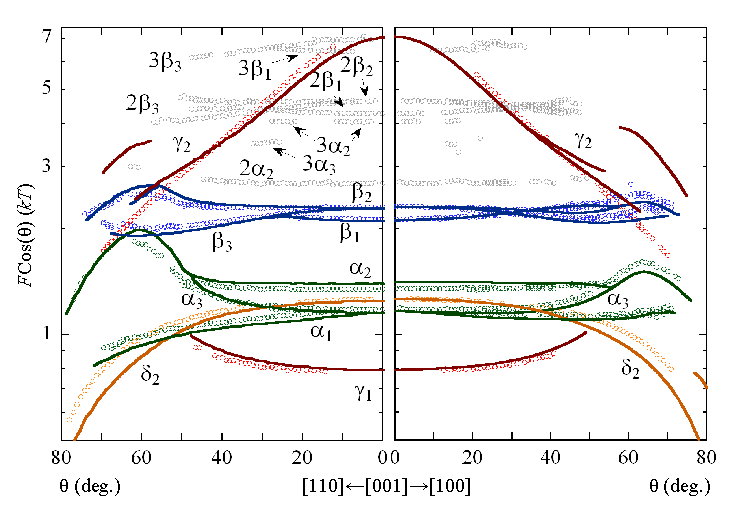
\includegraphics[scale=0.9]{Chapter-dHvABaFe2P2/Figures/AngleDepMeasurements/AngleSweepRigidShift/AngleSweepRigidShift}
        \caption{\ac{dHvA} frequencies multiplied by $\cos(\theta)$. Solid lines are rigidly shifted \ac{DFT} calculations, open circles are measured data. $H$ field directed along $[001]$ towards (a.) $[001]\rightarrow[100]$ and (b.) $[001]\rightarrow[110]$.}
        \label{Fig:ResD:AngleSweepRigidShift}
    \end{center}
\end{figure}

In order to obtain the correct shape of Fermi surface, the \ac{DFT} calculations need to be tweaked. One technique is to apply small band-specific rigid energy shifts, which, in most cases is enough to bring the \ac{DFT} in line with the experimental data. Figure~\ref{Fig:ResD:AngleSweepRigidShift} shows the rotation plots which rotate towards both the 100 and 110 directions along with appropriately shifted calculations. Table~\ref{Tab:ResD:EnergyShifts} lists those energy shifts.
\begin{table}
    \begin{center}
        \caption{Rigid energy shifts required to match the \ac{DFT} calculations with the measured data.}
        \begin{tabular}[htbp]{llr}
\toprule
Band    & \multicolumn{2}{l}{Energy Shift (Ry)} \\
\midrule
1       &       & -0.0083      \\
2       & Wide  & 0.0          \\
        & Narrow & -0.0038     \\
3       &       & 0.0043       \\
4       &       & 0.0050        \\
\bottomrule
        \label{Tab:ResD:EnergyShifts}
        \end{tabular}
    \end{center}
\end{table}

Band $2$ in this case has two separate shifts specified in two different regions of the \ac{BZ}. The rotation plot for the wider orbit located at the edge of the \ac{BZ} was calculated with no energy shift and the narrow part of the Fermi surface around the $\Gamma$ point was calculated with a shift of $\unit{0.0038}{Ry}$. This provides a reasonable match for the rotation plot where we can apply the shift to the two regions discretely, however is proves problematic when we wish to study intermediate areas since it is not clear how the Fermi surface varies between the two regions. A technique for applying appropriate energy shifts throughout the \ac{BZ} is explored in the next section.

\begin{figure}[htbp]
    \begin{center}
        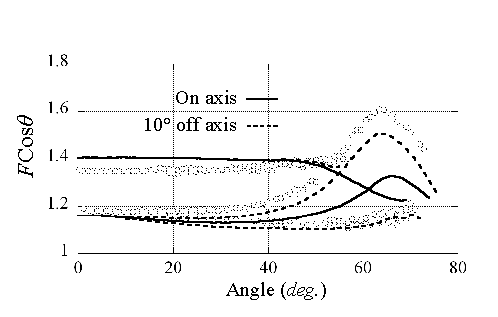
\includegraphics[scale=0.9]{Chapter-dHvABaFe2P2/Figures/AngleDepMeasurements/BaselMisalignment/BaselMisalignment}
        \caption{Portion of the measured \ac{FFT} peaks taken towards the `$[100]$' direction. Superimposed is angle plots calculated from \ac{DFT}. Solid is calculated for the field rotating down to $[100]$, dotted is rotated down to 10\degree off $[100]$ in the basel plane.}
        \label{Fig:ResD:BaselMisalignment}
    \end{center}
\end{figure}
For the $[100]$ direction it became apparent from the fact that the \ac{DFT} and the measured curves were qualitatively different that the field was not perfectly aligned with the $[100]$ axis of the sample. Figure~\ref{Fig:ResD:BaselMisalignment} shows how the measured data (circles) does not align well with the plots calculated for rotations towards $[100]$ (solid) but does align well with plots towards an axis which is rotated \unit{10}{\degree} within the $ab$-plane from the $[100]$ direction. A \unit{10}{\degree} misalignment is within the estimated basel alignment error for the microscope images. The data will continue to be labelled as in the $[100]$ plane however for convenience.

In the first place, these shifts were applied as they conveniently and effectively corrected the Fermi surface energies, however the question arises as to whether there is any physical significance to be attached to them. The technique of rigid energy corrections has been applied to previous measurements on LaFePO\cite{Carrington2009} and SrFe$_2$P$_2$\cite{Analytis2009} both of which are highly two dimensional systems that exhibit relatively strong nesting characteristics. This is in contrast with measurements on CaFe$_2$P$_2$\cite{Coldea2009} which has a highly three dimensional Fermi surface and no nesting vector. Furthermore the bulbous area of the three dimensional hole surface in \BaFeP which does not nest requires no shifting of the Fermi surface to match \ac{DFT} calculations, whereas the nested neck portion does require a shift. This correlation between nesting and shifts in calculated energy make the spin-density-wave fluctuations that are associated with the nesting phenomena an obvious candidate for the cause of the discrepancy between \ac{DFT} calculation and experiment.


\subsubsection{Shifting the \ac{DFT} calculations proportional to orbital character}
\label{Sec:ResD:ShiftingDFTPropToOrbitalCharacter}

Figure~\ref{Fig:ResD:Band2DCharacter} shows the partial orbital character for for each of the bands along the path of Fermi surface contour in a $[110]$ slice through the \BaFeP \ac{BZ} as a function of $k_z$. The top row of plots show the character broke down by atomic contribution, the middle row is broken down by the $s$, $p$, $d$ and $f$ contributions to the iron contribution and the bottom row breaks down the iron $d$ character into its sub orbitals.
\begin{figure}[htbp]
    \begin{center}
        \includegraphics[scale=0.95]{Chapter-dHvABaFe2P2/Figures/AngleDepMeasurements/BandCharacterVsKz/AllBandCharacterVsKz}
        \caption{Partial characters along the Fermi surface contour in the 110 slice (shown in insets) vs. $k_z$. Top row is the chaacrter broken down by each atom, middle row is the iron contribution broken down into the $l$ orbital contributions, the bottom row is the iron $d$ orbital contributions broken down into its suborbitals.}
        \label{Fig:ResD:Band2DCharacterVsKz}
    \end{center}
\end{figure}
We can see the vast majority of Fermi surface chaarcter is due to the iron atomic contributions with some phosphor for bands 2 and 3 which corresponds well to the notion of FeP conducting planes \TODO{Why does the total not sum to 1?}. For all the bands, the overwhelming majority of the contribution from the iron atoms is from the $d$ orbitals and so other contributions are ignored.

Band $2$ has very little basel-plane \Dxy and \DxTwoyTwo character close to the Fermi level but shows a significant amount of \DzTwo character at the wide region of the Fermi surface and \DxzDyz character at the narrow region. Evidently, energy shifts could be applied which are scaled to either the \DzTwo and \DxzDyz orbital character in order that we obtain a smooth energy shift transition between the narrow and wide regions discussed previously. 

Energy shifts were applied across the full three dimensional \ac{BZ} for band $2$ using the following two scalings which were determined by trial and error fitting of the data,
%%
\begin{align*}
\textrm{\DzTwo:}\quad \Delta\epsilon &= 0.002 - 0.0052 \left[1 - \frac{\epsilon - 0.033}{0.2205 - 0.033}\right] \\
\textrm{\DxzDyz:}\quad \Delta\epsilon &= 0.002 - 0.0052 \left[\frac{\epsilon - 0.0946}{0.3135 - 0.0946}\right]
\end{align*}
%%
Note that these scalings ensure that the energy shift applied varies between \unit{-32}{\milli Ry} and \unit{2}{\milli Ry} which are slightly different to the values applied when rigidly shifting the band. This is due to the fact that the Fermi surface area measured in the narrow region is affected more and more by the size of the Fermi surface in the wide region (and vice-versa) as the azimuthal angle gets higher. The calculated area deviates from the measured area which results in the crossing of the calculated rotation plot with the measured rotation plot shown in the first panel of figure~\ref{Fig:ResD:Band2DCharacterRigidComparison}. So when the rigid shifts were being determined, values were chosen which best lines up along the full length of the curve -- one which will be slightly lower than if we were to match the plots exactly at $\theta=0^\circ$.

\begin{figure}[htbp]
    \begin{center}
        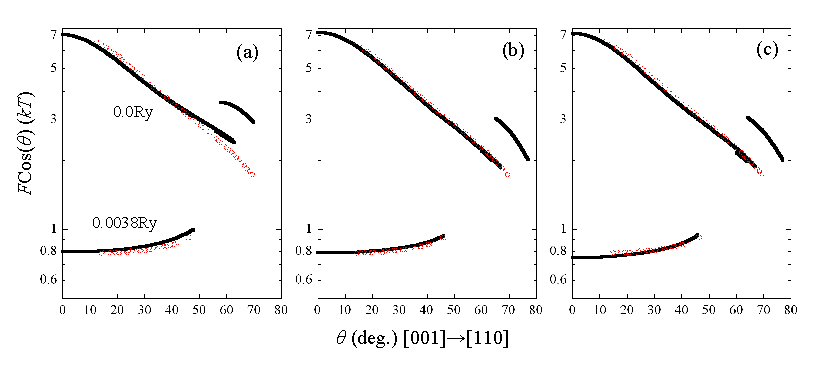
\includegraphics[scale=0.8]{Chapter-dHvABaFe2P2/Figures/AngleDepMeasurements/BandCharacterRotPlot/Band2_110_RotPlot_Comparison}
        \caption{dHvA frequencies for band 2 multiplied by the cosine of the angle of the $H$ field. $H$ field directed along $[001]\rightarrow[110]$. Open circles are measured data, solid lines represent (a) rigidly shifted \ac{DFT} calculations, (b) \ac{DFT} calculations shifted proportional to \DzTwo orbital character, (c) \ac{DFT} calculations shifted proportional to \DxzDyz orbital character.}
        \label{Fig:ResD:Band2DCharacterRigidComparison}
    \end{center}
\end{figure}

The second and third panels of figure~\ref{Fig:ResD:Band2DCharacterRigidComparison} show the rotation plots calculated with the energy shifts applied proportional to \DzTwo and \DxzDyz orbital character respectively. We observe a much better alignment of the measured and calculated data for all angles. Figure~\ref{Fig:ResD:BandCharacterFSShiftComparison} shows the Fermi surfaces before and after shifting using the rigid energy shifts for bands $1$, $3$ and $4$ and using shifts scaled to \DzTwo orbital character for band $2$. Figure~\ref{Fig:ResD:FullBandCharacterFermiSurface} shows the assembled unit cell for \BaFeP from the corrected \ac{DFT} calculations and figure~\ref{Fig:ResD:ShiftedBandStructure} shows the shifted band structure for the bands that cross the Fermi level.
%%
\begin{figure}[htbp]
    \begin{center}
        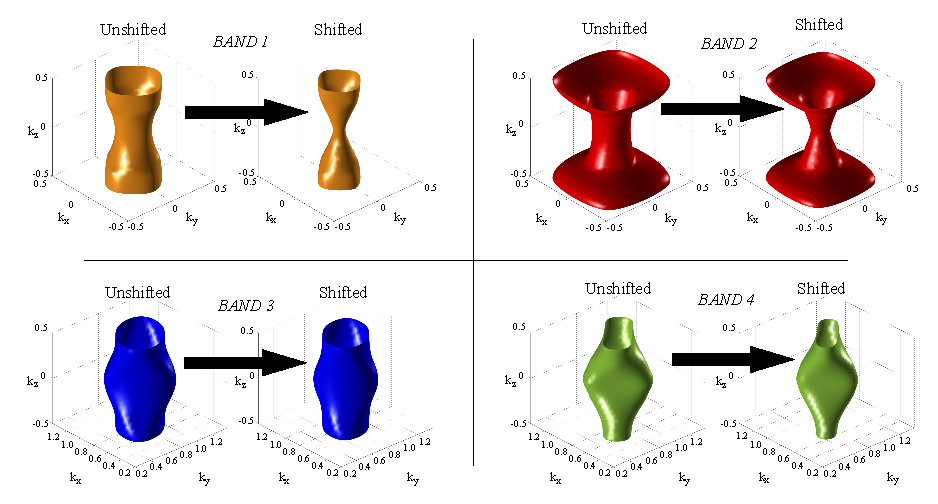
\includegraphics[scale=0.8]{Chapter-dHvABaFe2P2/Figures/AngleDepMeasurements/BandCharacterFermiSurface/BandCharacterFermiSurfaceShiftComparison}
        \caption{Comparison of Fermi surfaces according to \ac{DFT} calculations both before and after shift corrections are applied. Rigid shifts are applied to bands 1, 3, 4 and shifts proportional to \DzTwo character are applied to band 2.}
        \label{Fig:ResD:BandCharacterFSShiftComparison}
    \end{center}
\end{figure}
%%
\begin{figure}[htbp]
    \begin{center}
        \includegraphics[scale=0.7]{Chapter-dHvABaFe2P2/Figures/AngleDepMeasurements/BandCharacterFermiSurface/FullBandCharacterFermiSurface}
        \caption{Fully assembled Fermi surface in the first \ac{BZ} of \BaFeP as determined by \ac{DFT} calculations corrected by either rigid energy shifts (bands 1, 3, 4) or shifts proportional to \DzTwo character (band 2)}
        \label{Fig:ResD:FullBandCharacterFermiSurface}
    \end{center}
\end{figure}
%%

The final corrections show the \ac{DFT} calculations being adjusted in size only for the electron and inner hole surfaces with overall shrinking of volume, the outer hole surface is adjusted in shape as well. Volume calculations as a percentage of the \ac{BZ} are given for each of the Fermi surfaces before and after shifting in table~\ref{Table:ResD:FermiSurfaceVolumes},
\begin{table}
    \begin{center}
           \caption{Volumes of the shifted and unshifted Fermi surfaces as a percentage of \ac{BZ} volume.}
        \begin{tabular}[htbp]{lrrr}
\toprule
Band    & Unshifted    & Shifted \DzTwo    & Shifted \DxzDyz \\
\midrule
1  & 5.54\%    & 2.28\%    & 2.28\%    \\
2  & 10.37\%   & 9.74\%    & 9.64\%    \\
3  & (-)9.58\% & (-)7.89\% & (-)7.89\% \\
4  & (-)6.39\% & (-)4.49\% & (-)4.49\% \\
\midrule
Total & -0.065\%    & -0.352\%  & -0.450\%  \\
\bottomrule
        \label{Table:ResD:FermiSurfaceVolumes}
        \end{tabular}
    \end{center}
\end{table}
The volumes compensate better before the shifts by a small amount ($\sim$\unit{0.4}{\%}) with the shifts proprtional to \DxzDyz being slightly closer to the unshifted volume.

\section{Obtaining the Fermi surface for members of the \BaFePAs series}

We can use existing literature measurements of the Fermi surface at $x=0.38$ from Yoshida \etal \cite{Yoshida2010}, $x=0.63$ from Analytis \etal \cite{Analytis2010c} and a range between $0.4 < x < 1.0$ from Shishido \etal \cite{Shishido2010} to obatain an approximate relation for the size of Fermi surface orbits across the \BaFePAs series. Figure~\ref{Fig:ResD:SeriesRecipe} shows the maximum and minimum orbit sizes with the field along the $c$-axis from these papers along with data presented in this thesis.
\begin{figure}[htbp]
    \begin{center}
        \includegraphics[scale=1.1]{Chapter-dHvABaFe2P2/Figures/AngleDepMeasurements/SeriesRecipe/SeriesRecipe}
        \caption{Left panel shows the trend in electron orbit size at $\theta=0\degree$ over the series, right panel show the hole orbit size trends. Dotted lines show linear fits to the data.}
        \label{Fig:ResD:SeriesRecipe}
    \end{center}
\end{figure}
It may be possible to apply a linear scaling to determine the intermediate orbit sizes however there are a number of assumptions that need to be made. 

Firstly we cannot apply Vegard's law beyond a structural transition in the series meaning we cannot extrapolate to the orthorhombic state at the low $x$ end of the phase diagram. The measurement by Yoshida et al. at $x=0.38$ roughly coincides with the edge of the orthorhombic transition as shown in figure~\ref{Fig:ResD:PhaseDiagram} but was found to be tetragonal and so we can use to to define the lower limit for the extrapolation at low temperatures. There is also a so called `collapsed tetragonal phase' which occurs in the \BaFeAs at a pressure \unit{27}{\giga\pascal}\cite{Mittal2011} at \unit{33}{\kelvin} which could present a problme as we apply chemical pressure. The optimal \Tc of \BaFeAs under pressure is $\sim$\unit{5}{\giga\pascal}~\cite{Colombier2009} and optimal \Tc for the \BaFePAs series is $x\sim0.3$, and so we can very approximately place $x=1$ corresponding to $\sim$\unit{7}{\giga\pascal} which is about half of that required for the collapsed phase transition. Moreover the author is not aware of any reports of the collapsed phase being observed in the \BaFePAs series at atmospheric pressure and so we assume that this is the case. 

There is also the problem of the third hole surface around the $\Gamma$ point which appears in \ac{DFT} calculations. Although it has not been observed in any of the measurements, this is to be expected since electron surfaces generally scatter more and so have a weaker signal to electron pockets and also it may be close in size and shape to other hole surfaces making it difficult to pick out with current \ac{ARPES} resolution.

Looking at figure~\ref{Fig:ResD:SeriesRecipe} we see some inconsistencies which may also throw some doubt onto such a linear fit. Key points from Yoshida \etal are measured from \ac{ARPES} and not \ac{dHvA}. As they were measured at \unit{10}{\kelvin}, this means that the Fermi surface is measured in the superconducting state and not the field suppressed normal state which is the case for the \ac{dHvA} data. It is not clear if this results in different Fermi surfaces. It also should be noted that a linear extrapolation of $\delta$ suggests that it will become more three dimentional as it goes below $x=0.38$, however this does not appear to be supported by the \ac{DFT} results which show it remaining quasi-two dimensional. 

With the above (many) caveats in mind, we can determine a series of linear laws which would approxmately determine the orbit sizes for $0.38 < x < 1.0$ by applying fits to the data in figure~\ref{Fig:ResD:SeriesRecipe}. The results of these fits are given in table~\ref{Table:ResD:SeriesRecipeFits}.
\begin{table}
    \begin{center}
           \caption{Linear relations to determine orbit sizes. Coefficients are of the form $F=mx+c$.}
        \begin{tabular}[htbp]{lrr}
\toprule
Orbit   & $m$   & $c$   \\
\midrule
$\delta_{\textrm{max}}$ & 0.081 & 1.169 \\
$\delta_{\textrm{min}}$ & -1.766 & 1.841 \\
$\gamma_{\textrm{max}}$ & 4.339 & 3.111 \\
$\gamma_{\textrm{min}}$ & 0.698 &  0.071 \\
$\beta_{\textrm{min}}$ & 0.749 & 1.352 \\
$\beta_{\textrm{max}}$ & 0.811 & 1.489 \\
$\alpha_{\textrm{max}}$ & 0.495 & 0.646 \\
$\alpha_{\textrm{min}}$ & 0.946 & 0.404 \\
\bottomrule
        \label{Table:ResD:SeriesRecipeFits}
        \end{tabular}
    \end{center}
\end{table}




\section{Susceptibility calculations}
    \label{Sec:ResD:SubsceptibilityCalculation}

To verify that we do get enhanced susceptibility, which may lead to a spin-density wave state, the $q$-dependant susceptibility -- described in section~\ref{Sec:Theo:Susceptibility} -- was calculated. Since the Lindhard function takes the sum over all energies in the \ac{BZ}, there may be some concern that the rather crude adjustments to the \ac{DFT} calculations performed in the previous section -- which have only been verified to be correct for energies at the Fermi surface -- may give erroneous results. However the nature of the Lindhard function means that far greater weight is given to energies that are near the Fermi surface. Figure~\ref{Fig:ResD:ShiftedBandStructure} shows the `spaghetti plot' with the energies tweaked as described in the previous section. We see that there are discontinuities in band 2, most notably between $Z$ and $\Sigma_1$, due to the correction applied proportional to the \DzTwo{} character, however these are reasonably far from the Fermi level and so should not affect the calculations significantly.
\begin{figure}[htbp]
    \begin{center}
        \includegraphics[scale=0.9]{Chapter-dHvABaFe2P2/Figures/AngleDepMeasurements/ShiftedBandStructure/ShiftedBandStructure}
        \caption{Band structure for the bands that cross the Fermi surface shifted to fit the dHvA data. (a) and (b) give an idea of the granularity of the \WIEN{} calculation at the Fermi surface. Inset shows the path around the \ac{BZ}.}
        \label{Fig:ResD:ShiftedBandStructure}
    \end{center}
\end{figure}

Calculations were performed using the \code{calc_x0.m} code described in section~\ref{Sec:Exp:Susceptibility} using a $93\times93\times93$ grid of energy values that covered the first \ac{BZ}. We will need to smooth over the granularity of the \WIEN{} band model since for the imaginary part at least, the calculation is very sensitive to slight imperfections in cancellation near the Fermi energy. Referring to figure~\ref{Fig:ResD:ShiftedBandStructure}, there are two regions in the marked (a) and (b) which show points around the Fermi level as they are spaced in the $93\times93\times93$ model. (a) is particularly steep and has a $\Delta \epsilon/\Delta\textrm{pt.} = \unit{0.0760}{\electronvolt}$ and (b) is more typical of the gradient at the Fermi level and has $\Delta \epsilon/\Delta\textrm{pt.} = \unit{0.0368}{\electronvolt}$. So the energy scale that will need to compensated is $\sim$\unit{2-5\ten{-3}}{\textrm{\textrm{Ry}}}.

\begin{figure}[htbp]
    \begin{center}
        \includegraphics[scale=0.9]{Chapter-dHvABaFe2P2/Figures/Susceptibility/RangeDeltaOmega/RangeDeltaOmega}
        \caption{Qualitative plots of the real and imaginary part of the Lindhard susceptibility calculated at $k_z=\pi$ for $T=\unit{157}{\kelvin}$ and a range of $\delta$ and $\omega$ values.}
        \label{Fig:ResD:RangeDeltaOmega}
    \end{center}
\end{figure}

Susceptibility was calculated for a wide range of magnitudes of $\delta$ and $\omega$ in order to gauge qualitative behaviour with the resulting plots shown in figure~\ref{Fig:ResD:RangeDeltaOmega}. Both the real and imaginary parts undergo qualitative changes as the parameters are adjusted above the spacing corresponding to the typical gap in energy between points. The imaginary part also undergoes a qualitative change when $\omega$ falls below \unit{1\ten{-5}}{\textrm{Ry}} and there is also an increase in noise when $\delta$ falls below a similar energy threshold. We continue using $\delta=1\ten{-3}$ and $\omega=1\ten{-3}$ which correspond approximately the energy scale of the spacing as well as the energy scale of the temperature smearing.

\begin{figure}[htbp]
    \begin{center}
        \includegraphics[scale=0.9]{Chapter-dHvABaFe2P2/Figures/Susceptibility/2DSusceptibility/2DSusceptibilityPlusAltKz}
        \caption{Real and imaginary part of the Lindhard susceptibility are plotted on the left and right respectively. Upper panels are at $k_z=\pi$ and lower are at $k_z=0$. For these calculations $\delta=1\ten{-3}$, $\omega=1\ten{-3}$ and $T=\unit{157.88}{\kelvin}$. Insets show contour plots for the respective surface plots.}
        \label{Fig:ResD:2DSusceptibility}
    \end{center}
\end{figure}
The upper panel of figure~\ref{Fig:ResD:2DSusceptibility} shows the quantified plots for the real and imaginary parts of the susceptibility at the chosen values of $\delta$ and $\omega$. The contour plots in the insets show the two-fold symmetry due to the choice of $k_z=\pi$. Unlike LaFeAsOF where the two dimensional approximation is a good one, this is not necessarily the case for \BaFeP{} which features a strongly three-dimensional hole band and some warping of the electron bands. The lower panels present the same calculation performed at $k_z=0$ which shows little change other than a rotation of the susceptibility bias due to the screw symmetry of the electron bands.

\begin{figure}[htbp]
    \begin{center}
        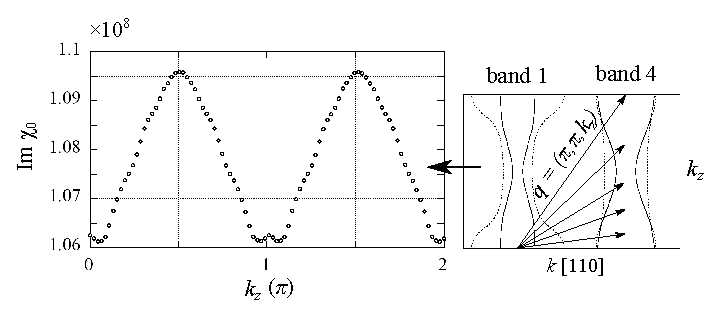
\includegraphics[scale=0.7]{Chapter-dHvABaFe2P2/Figures/Susceptibility/NestingVector/NestingVector}
        \caption{Left panel shows the imaginary part of the Lindhard susceptibility between bands summed with their reciprocals for $q=(\pi, \pi, k_z)$ over the height of the \ac{BZ}. We see enhancements at $k_z=\pi/2,3\pi/2$ for bands 1-4 and 2-3 and at $k_z=0,\pi,2\pi$ for bands 2-3 and 2-4.}
        \label{Fig:ResD:NestingVector}
    \end{center}
\end{figure}
To verify that there is indeed a nesting conditions at some $k_z$ for $q=(\pi, \pi, k_z)$ figure~\ref{Fig:ResD:NestingVector} presents the imaginary part of the susceptibility vs. $k_z$ for a range of nesting vectors. Each coupling of bands is summed both ways --- e.g. 4-1 is summed with 1-4 --- and plotted in order to obtain the residual difference due to $\omega$. Unsurprisingly, we see that self coupling results in very little weight with hole-hole and electron-electron coupling also resulting in little weight. The strongest component is due to bands 2-4 which also demonstrates a strong enhancement of around $25\%$ at $k_z=0,\pi,2\pi$. Band 2 also couples strongly with band three at the same $q$ vectors with around a $17\%$ enhancement. Band 1 couples strongly with band 4 but at $k_z=\pi/2,3\pi/2$ with the largest enhancement of around $38\%$. Band 1 also couples less strongly with band $3$ at the same $k_z$ with an enhancement of around $15\%$. The total susceptibility is determined mostly by the coupling of band 2 but only has a relatively moderate enhancement of around $7.4\%$ at $k_z=0,\pi,2\pi$.

Figure~\ref{Fig:ResD:ZSlices} shows cross sections of the final corrected Fermi surfaces showing the basal-plane at the bottom of the unit cell ($k_z=0$), quarter of the way up, ($k_z=0.25$) and halfway up ($k_z=0.5$). The inner hole surface (band 1) at $k_z=0.5$ directly matches the size and shape of the inner electron surface (band 4) at $k_z=0.25$ which is the likely cause of the strong enhancement observed in the susceptibility. Moreover, the bands share similar predominant \DxzDyz{} orbital character. The strong enhancements between bands 2 and 4 are also shown in the figure as a dashed arrow.

\begin{figure}[htbp]
    \begin{center}
        \includegraphics[scale=0.9]{Chapter-dHvABaFe2P2/Figures/AngleDepMeasurements/ZSlices/ZSlices}
        \caption{Cross sections of the corrected Fermi surface in the $ab$ plane (panels 1, 2 and 3) and in the $[110]$ plane (panel 4). Markings correspond to the orbital character of the Fermi surface slices. Two nesting vectors are shown as long arrows.}
        \label{Fig:ResD:ZSlices}
    \end{center}
\end{figure}

These enhancements at $q=(\pi, \pi)$ show that partial nesting does indeed occur in this material demonstrating that this condition alone is not sufficient for superconductivity to occur. This concludes the Fermiology results, we now move onto the mass enhancements.




\section{Determining the spin mass}

Following the method in section~\ref{Sec:Exp:MeasuringSpinMass} we begin by taking a variety of spin masses using the cylindrical approximation. Figure~\ref{Fig:ResD:Band4SpinMassCylindrical} shows \ac{FFT} amplitudes for a portion of the $\alpha$ electron pocket taken over a range of angles towards the $[100]$ direction. The shaded areas are bound to the areas where we believe the amplitudes go to zero as defined by the overall shape of the curve and the splitting of the peaks. The upper panel shows the particular oscillation that most closely matches the zeros in the data as well as its upper and lower bounds to quantify the possible error. The lower panel shows the next and previous set of oscillations in order to demonstrate that the selected oscillation in the top panel is indeed the best fit. In the cylindrical case the best fit is given by \TODO{XXXXX} with an error of \TODO{XXXX}.
\begin{figure}[htbp]
    \begin{center}
        
\includegraphics[scale=0.9]{Misc/TODO}
        \caption{Measured amplitude of \ac{FFT} peaks across a range of angles for the portion of data shown in the inset. Curves corresponding to the $A_S$ term calculated using the cylindrical apporximation are superimposed. Upper panel shows the best fitting data and its bounds, the lower portion shows fitting to the next oscillation along which clearly demonstrates the misalignment. Shaded areas are zones where we believe the spin zeros are located in the data.}
        \label{Fig:ResD:Band4SpinMassCylindrical}
    \end{center}
\end{figure}
We now contrast this with a spin mass determination using a band mass calculated from \ac{DFT}. Figure~\ref{Fig:ResD:DFTBandMassBand4} shows the band mass as calculated from the shifted \ac{DFT} energies for band 4. On the plot is an order 8 polynomial fit as well as the corresponding cylindrical approximation curve for comparison.
\begin{figure}[htbp]
    \begin{center}
        \includegraphics[scale=0.9]{Chapter-dHvABaFe2P2/Figures/Mass/DFTBandMassBand4/DFTBandMassBand4}
        \caption{Band masses calculated from \ac{DFT} of band 4 taken over a range of angles rotating towards the $[100]$ direction. A fit to and order 8 polynomial is shows as well as a comparitive fit suing the cylindrical approximation.}
        \label{Fig:ResD:DFTBandMassBand4}
    \end{center}
\end{figure}
Taking the polynomial from the fit to the \ac{DFT} band mass calulcations as the band mass for the inspection of the $A_S$ term, figure~\ref{Fig:ResD:SpinMassFromDFTBand4} shows the revised best fit. Now the fit values gives a spin mass of \TODO{XXXX} with an error pf \TODO{XXXX}.
\begin{figure}[htbp]
    \begin{center}
        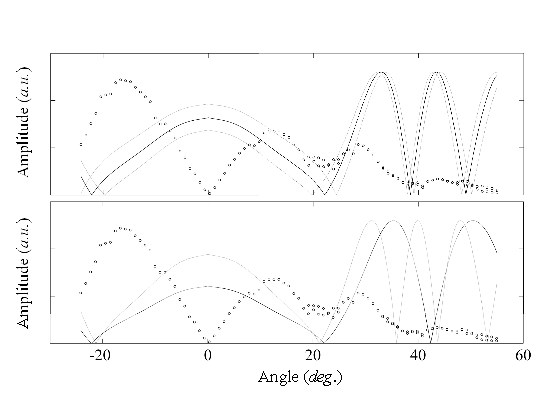
\includegraphics[scale=0.8]{Chapter-dHvABaFe2P2/Figures/Mass/SpinMassBand4/SpinMassBand4}
        \caption{Measured amplitude of \ac{FFT} peaks across a range of angles for the portion of data shown in the inset.  Curves corresponding to the $A_S$ term calculated using the cylindrical apporximation are superimposed. Upper panel shows the best fitting data and its bounds, the lower portion shows fitting to the next oscillation along which clearly demonstrates the misalignment. Shaded areas are zones where we believe the spin zeros are located in the data.}
        \label{Fig:ResD:SpinMassFromDFTBand4}
    \end{center}
\end{figure}
Given that a more accurate fit is obtained by using the \ac{DFT} calculated band masses, table~\ref{Table:ResD:SpinMassValues} shows more spin mass values calculated using this technique with the full graphs given in Appendix~\ref{Appendix:SpinMassPlots}.
\begin{table}
    \begin{center}
           \caption{Spin mass values calculated using inspection of measured data. Values calculated from \ac{DFT} were used for the band mass term.}
        \begin{tabular}[htbp]{ll}
\toprule
Band    &   $m^*_S$ \\
\midrule
\TODO{XXXX} & \TODO{XXXX} \\
\bottomrule
        \label{Table:ResD:SpinMassValues}
        \end{tabular}
    \end{center}
\end{table}



\section{Determining the thermal effective mass}


\subsubsection{Basic \ac{LK} formula fitting}

A series of field sweeps were taken with $H$ at \unit[12]{\degree}, \unit[28]{\degree} and \unit[46]{\degree} from $[001]$ in the $[110]$ direction. These were performed at a variety of temperatures from base ($\approx\unit[0.3]{K}$) to above \unit[2]{K}. Corrections were applied as detailed in section\ref{Sec:Exp:TemperatureCorrection}. \Fig~\ref{Fig:ResD:SimpleLKFits} shows the Fourier amplitude of various peaks as a function of temperature along with fits to equation~\ref{Eqn:Exp:TempTermOscillationAmp}. The field range for the FFT was was necessarily large enough that individual peaks did not overlap and also could be observed across a reasonable range of temperatures but also small enough so that the $B$ dependent Dingle factor did not play too large a role and so an average $B$ field can be assumed. The results from these fits are shown in table \ref{Tab:ResD:EffectiveMassResults} along with the fit ranges. All FFTs in the plot were taken over an interval of \unit[12--18]{T} with the exception of the $\gamma_2$ fit which was taken between \unit[16-18]{T} so as to attain an appreciable peak. The standard deviation as calculated by randomly varying the temperature values by the estimated error (\unit[0.06]{K}) 1000 times and then taking the standard deviation of the fitted $m^*$ values.
\begin{figure}[htbp]
    \begin{center}
        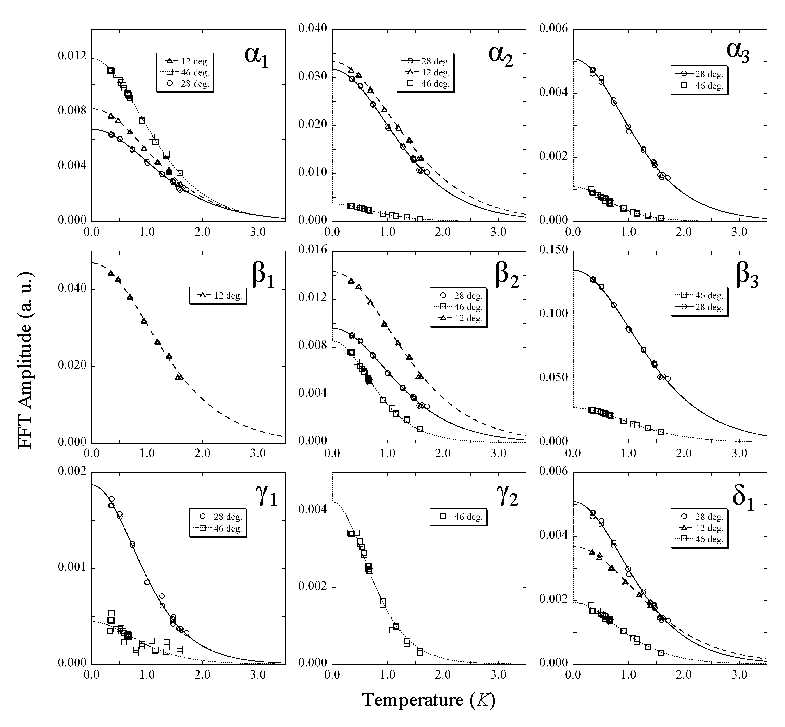
\includegraphics[scale=0.9]{Chapter-dHvABaFe2P2/Figures/Mass/SimpleLKFits/SimpleLKFits}
        \caption{Fits to the temperature dependant part of the \LK formula. }
        \label{Fig:ResD:SimpleLKFits}
    \end{center}
\end{figure}
Table \ref{Tab:ResD:EffectiveMassResults} also shows gives a result, marked with a dagger, taken with a different field range. These fits give quite different values for the effective mass, indicating that the average field approximation is not a valid one.

\subsubsection{Retrofitting ansatz LK formulae}

The measurements presented in the previous section were further refined using the the ansatz LK formulae as described in section~\ref{Sec:Exp:LKRetrofitting}. \Fig~\ref{Fig:ResD:DingleTermExtractionFits} shows some sample fits used to extract the Dingle terms used in the ansatz fit functions.
\begin{figure}[htbp]
    \begin{center}
        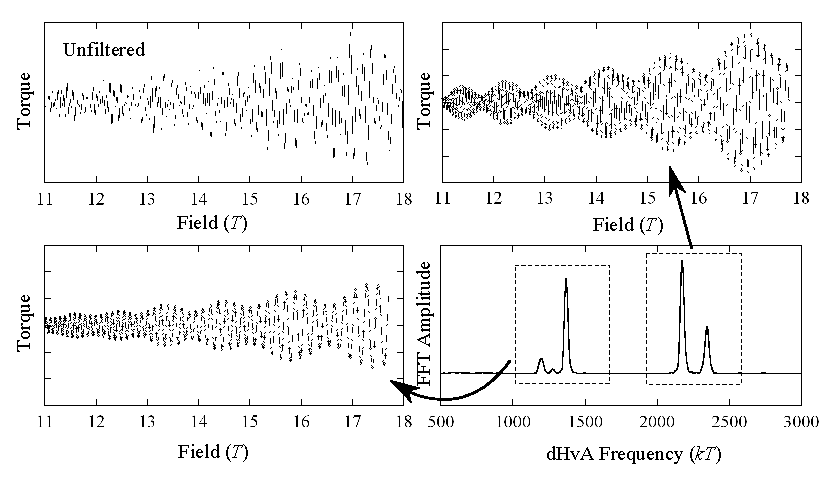
\includegraphics[scale=0.9]{Chapter-dHvABaFe2P2/Figures/Mass/FittingDingleTerm/FittingDingleTerm}
        \caption{Top left panel shows torque data for data taken at \unit[12]{\degree} towards the $[110]$ direction at \unit[0.35]{K} with a polynomial background subtracted. Bottom right shows the FFT and the two filter windows to produce the filtered torque plots in the top right and bottom left. Filtered plots are fitted to extract the Dingle term for each frequency.}
        \label{Fig:ResD:DingleTermExtractionFits}
    \end{center}
\end{figure}
Table\ref{Tab:ResD:EffectiveMassResults} lists the extracted Dingle terms for each peak of the Fermi surface and the subsequent results of the retrofitted calculations for the effective masses. The various field limits were chosen in order to either obtain a clearly delimited peak in the lower field cases or to obtain a signal from a weak peak in the higher field cases.


\subsubsection{`Microfitting' the LK formula}

A second attempt at refining the LK fits was performed by applying the microfit technique desribed in section~\ref{Sec:Exp:LKMicrofitting}. $1.5$ oscillations were fit at a time Filtering the data beforehand is not always straightforward due to close proximity of neighbouring peaks. The stronger peaks from the $\alpha$ and $\beta$ Fermi surfaces show banding of the masses and a clear trending of the results to one of a few values which have been highlighted in yellow. Data in these regions were averaged to give the values in table \ref{Tab:ResD:EffectiveMassResults}.

All filtered using function $\textit{F}_{\textrm{filt}}(x) = \textit{F}(x) \times 1/2 [\tanh{(\pi(x - x_{\textrm{low}})/w)} + \tanh{(-\pi(x - x_{\textrm{high}})/w})]$ where $\textit{F}$ is the Fourier transform of the torque data, $x$ is the dHvA frequency, $x_{\textrm{low}}$ and $x_{\textrm{high}}$ are the lower and upper limits of the filter range respectively and $w$ determines the trail off slope of the filter function. For all measurements $w=10$.
%%
\begin{figure}[htbp]
    \begin{center}
        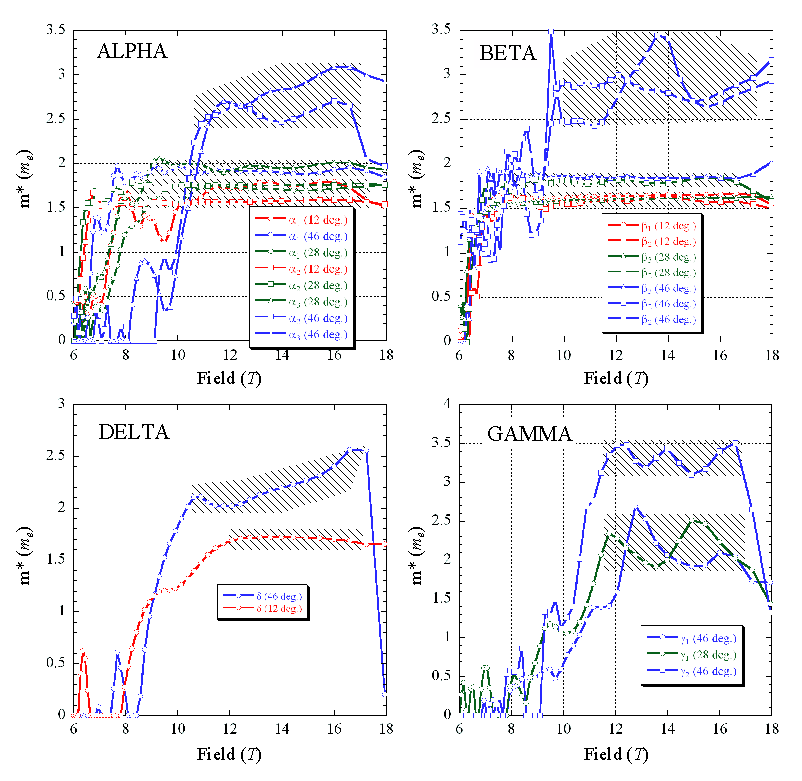
\includegraphics[scale=0.7]{Chapter-dHvABaFe2P2/Figures/Mass/MicroFits/MicroFits}
        \caption{Effective temperature dependant masses extracted from fits to between one and three dHvA oscillations in the measured data. See Appendix\ref{Appendix:MicroFitParams} for a full list of parameters for each set of fits.}
        \label{Fig:ResD:MicroFits}
    \end{center}
\end{figure}
%%
\begin{sidewaystable}
    \begin{center}
        \caption{Comparison of the three effective mass calculation techniques. First grey band shows the plain \LK fitted results, following white band details the retrofitted effective mass calculations, following grey band details the microfitted results, and the final band details the band masses from DFT calculations and the three results normalised to these band masses. Result marked with a dagger is repeated with a different field range. Entries marked `NA' had a signal too weak to extract an $\alpha$ value and so microfitting was not possible.}
{\small
        \begin{tabular}[htbp]{rrlrrrrrrrrrrrr}
\toprule
Angle	& Freq.	& Label	& $m^*_{\textrm{LK}}$	& $m^*_{\textrm{ret.}}$	& $\alpha$	& $B_{\textrm{min.}}$	& $m^*_{\textrm{mic.}}$	& $B_{\textrm{max.}}$	& $B_{\textrm{min.}}$	& Filt. Width	& $m^*_{\textrm{b}}$	& $\frac{m^*_{\textrm{LK}}}{m^*_{\textrm{b}}}$	& $\frac{m^*_{\textrm{ret.}}}{m^*_{\textrm{b}}}$	& $\frac{m^*_{\textrm{mic.}}}{m^*_{\textrm{b}}}$ \\
\midrule
12	& 1210	& $\alpha_1$	& \cellcolor[gray]{0.9} 1.49(2)$^\dagger$	& 1.69	& 58.68	& 8	& \cellcolor[gray]{0.9} NA	& \cellcolor[gray]{0.9} NA	& \cellcolor[gray]{0.9} NA	& \cellcolor[gray]{0.9} NA	& 1.04	& 1.43	& 1.63	& NA \\
12	& 1210	& $\alpha_1$	& \cellcolor[gray]{0.9} 1.71(3)	& 1.75	& 58.68	& 12	& \cellcolor[gray]{0.9} 1.75(3)	& \cellcolor[gray]{0.9} 17.0	& \cellcolor[gray]{0.9} 11.0	& \cellcolor[gray]{0.9} 1100--1240	& 1.04	& 1.64	& 1.68	& 1.68 \\
28	& 1269	& $\alpha_1$	& \cellcolor[gray]{0.9} 1.64(2)	& 1.68	& 59.60	& 12	& \cellcolor[gray]{0.9} 1.72(2)	& \cellcolor[gray]{0.9} 17.0	& \cellcolor[gray]{0.9} 11.0	& \cellcolor[gray]{0.9} 1200--1310	& 0.90	& 1.83	& 1.88	& 1.92 \\
46	& 1532	& $\alpha_1$	& \cellcolor[gray]{0.9} 1.86(3)	& 1.90	& 48.79	& 12	& \cellcolor[gray]{0.9} 1.92(2)	& \cellcolor[gray]{0.9} 17.0	& \cellcolor[gray]{0.9} 9.0	& \cellcolor[gray]{0.9} 1430--1585	& 1.00	& 1.86	& 1.90	& 1.92 \\
12	& 1372	& $\alpha_2$	& \cellcolor[gray]{0.9} 1.54(2)	& 1.58	& 45.99	& 12	& \cellcolor[gray]{0.9} 1.57(1)	& \cellcolor[gray]{0.9} 17.0	& \cellcolor[gray]{0.9} 8.0	& \cellcolor[gray]{0.9} 1320--1440	& 0.84	& 1.83	& 1.88	& 1.86 \\
28	& 1530	& $\alpha_2$	& \cellcolor[gray]{0.9} 1.69(2)	& 1.74	& 72.35	& 12	& \cellcolor[gray]{0.9} 1.75(2)	& \cellcolor[gray]{0.9} 17.0	& \cellcolor[gray]{0.9} 8.0	& \cellcolor[gray]{0.9} 1450--1650	& 0.93	& 1.81	& 1.87	& 1.88 \\
46	& 2017	& $\alpha_2$	& \cellcolor[gray]{0.9} 2.49(5)	& 2.56	& 61.06	& 12	& \cellcolor[gray]{0.9} 2.55(11)	& \cellcolor[gray]{0.9} 16.8	& \cellcolor[gray]{0.9} 10.5	& \cellcolor[gray]{0.9} 1970--2100	& 1.83	& 1.36	& 1.40	& 1.40 \\
28	& 1365	& $\alpha_3$	& \cellcolor[gray]{0.9} 1.85(3)	& 1.93	& 115.49	& 12	& \cellcolor[gray]{0.9} 1.97(3)	& \cellcolor[gray]{0.9} 17.0	& \cellcolor[gray]{0.9} 9.5	& \cellcolor[gray]{0.9} 1320--1440	& 1.18	& 1.56	& 1.63	& 1.67 \\
46	& 1930	& $\alpha_3$	& \cellcolor[gray]{0.9} 2.87(7)	& 3.04	& 149.39	& 12	& \cellcolor[gray]{0.9} 2.75(24)	& \cellcolor[gray]{0.9} 17.0	& \cellcolor[gray]{0.9} 10.7	& \cellcolor[gray]{0.9} 1890--1970	& 1.00	& 2.87	& 3.04	& 2.75 \\
12	& 2180	& $\beta_1$	& \cellcolor[gray]{0.9} 1.61(2)	& 1.65	& 51.12	& 12	& \cellcolor[gray]{0.9} 1.63(2)	& \cellcolor[gray]{0.9} 17.0	& \cellcolor[gray]{0.9} 8.0	& \cellcolor[gray]{0.9} 2100--2270	& 0.98	& 1.64	& 1.68	& 1.66 \\
12	& 2350	& $\beta_2$	& \cellcolor[gray]{0.9} 1.56(3)	& 1.62	& 102.36	& 12	& \cellcolor[gray]{0.9} 1.57(3)	& \cellcolor[gray]{0.9} 17.0	& \cellcolor[gray]{0.9} 9.0	& \cellcolor[gray]{0.9} 2270--2450	& 0.86	& 1.81	& 1.88	& 1.82 \\
28	& 2605	& $\beta_2$	& \cellcolor[gray]{0.9} 1.30(2)	& 1.87	& 102.36	& 6	& \cellcolor[gray]{0.9} 1.81(2)	& \cellcolor[gray]{0.9} 17.0	& \cellcolor[gray]{0.9} 8.5	& \cellcolor[gray]{0.9} 2555--2670	& 1.03	& 1.68	& 1.71	& 1.76 \\
46	& 3347	& $\beta_2$	& \cellcolor[gray]{0.9} 1.73(2)	& 1.76	& 34.08	& 12	& \cellcolor[gray]{0.9} 2.86(8)	& \cellcolor[gray]{0.9} 17.3	& \cellcolor[gray]{0.9} 10.0	& \cellcolor[gray]{0.9} 3250--3370	& 1.80	& 1.44	& 1.50	& 1.59 \\
46	& 3381	& $\beta_2$	& \cellcolor[gray]{0.9} 2.59(6)	& 2.69	& 94.57	& 12	& \cellcolor[gray]{0.9} 2.78(32)	& \cellcolor[gray]{0.9} 17.3	& \cellcolor[gray]{0.9} 10.0	& \cellcolor[gray]{0.9} 3365--2500	& 1.80	& 0.88	& 0.90	& 1.55 \\
28	& 2475	& $\beta_3$	& \cellcolor[gray]{0.9} 1.58(2)	& 1.61	& 48.81	& 12	& \cellcolor[gray]{0.9} 1.59(2)	& \cellcolor[gray]{0.9} 17.0	& \cellcolor[gray]{0.9} 8.0	& \cellcolor[gray]{0.9} 2400--2560	& 0.93	& 1.95	& 2.00	& 1.71 \\
46	& 2970	& $\beta_3$	& \cellcolor[gray]{0.9} 1.82(3)	& 1.86	& 40.03	& 12	& \cellcolor[gray]{0.9} 1.86(1)	& \cellcolor[gray]{0.9} 17.0	& \cellcolor[gray]{0.9} 8.5	& \cellcolor[gray]{0.9} 2850--3100	& 1.03	& 2.07	& 2.15	& 1.80 \\
28	& 912	& $\gamma_1$	& \cellcolor[gray]{0.9} 2.13(5)	& 2.22	& 104.38	& 12	& \cellcolor[gray]{0.9} 2.17(18)	& \cellcolor[gray]{0.9} 16.8	& \cellcolor[gray]{0.9} 11.3	& \cellcolor[gray]{0.9} 850--970	& -1.49	& -1.03	& -1.10	& -1.46 \\
46	& 1320	& $\gamma_1$	& \cellcolor[gray]{0.9} 2.19(3)	& 2.30	& 129.82	& 12	& \cellcolor[gray]{0.9} 2.00(37)	& \cellcolor[gray]{0.9} 16.8	& \cellcolor[gray]{0.9} 11.3	& \cellcolor[gray]{0.9} 1270--1370	& -2.04	& -0.91	& -0.95	& -0.98 \\
46	& 4497	& $\gamma_2$	& \cellcolor[gray]{0.9} 3.31(8)	& 3.32	& 91.06	& 16	& \cellcolor[gray]{0.9} 3.31(13)	& \cellcolor[gray]{0.9} 16.8	& \cellcolor[gray]{0.9} 12.2	& \cellcolor[gray]{0.9} 4400--4600	& -1.89	& -1.17	& -1.23	& -1.75 \\
12	& 1270	& $\delta$	& \cellcolor[gray]{0.9} 1.54(2)	& 1.64	& 173.00	& 12	& \cellcolor[gray]{0.9} 1.71(1)	& \cellcolor[gray]{0.9} 17.0	& \cellcolor[gray]{0.9} 12.0	& \cellcolor[gray]{0.9} 1250--1310	& -0.91	& -2.41	& -2.53	& -1.88 \\
28	& 1370	& $\delta$	& \cellcolor[gray]{0.9} 1.85(3)	& 1.93	& 115.49	& 12	& \cellcolor[gray]{0.9} NA	& \cellcolor[gray]{0.9} NA	& \cellcolor[gray]{0.9} NA	& \cellcolor[gray]{0.9} NA	& -0.98	& -1.89	& -1.97	& NA \\
46	& 1626	& $\delta$	& \cellcolor[gray]{0.9} 2.22(4)	& 2.33	& 126.02	& 12	& \cellcolor[gray]{0.9} 2.17(15)	& \cellcolor[gray]{0.9} 17.0	& \cellcolor[gray]{0.9} 10.5	& \cellcolor[gray]{0.9} 1590--1690	& -1.10	& -3.00	& -3.01	& -1.96 \\

\bottomrule
        \end{tabular}
}
        \label{Tab:ResD:EffectiveMassResults}
    \end{center}
\end{sidewaystable}



\section{Harmonic parametrisation of the Fermi surface}
    \label{Sec:ResD:TightBindingFits}

An analytic form for the Fermi surface can be obtained using a harmonic expansion of sin and cosine functions as described by Bergemann et al\cite{Bergemann2000}. Primarily this was done so as to provide a convenient way to reconstruct the Fermi surface without necessitating DFT calculations however the coefficients also bear some relation to the tight binding model hopping integrals. For strongly correlated systems the tight binding model is generally a poor one to use as it entirely ignores electron correlations. Nonetheless the expansion is as described as,
\begin{equation}
\label{Eqn:ResD:HarmonicExpansion}
k_F(\phi, \kappa) = \sum_{\substack{\mu,\nu \geq 0 \\ \mu \textrm{even}}}
    k_{\mu\nu}\cos\nu\kappa 
    \begin{cases}
        \cos{\mu\phi} \hspace{8pt} &(\mu\mod4 = 0) \\
        \sin{\mu\phi} \hspace{8pt} &(\mu\mod4 = 2)
    \end{cases}
\end{equation}
where $k_F$ is the Fermi surface in k-space, $\kappa = ck_z/2$, $c$ is the unit cell height and $\phi$ is the polar angle.

The two dimensional fits were performed using a least square fitting routine using MATLAB on the DFT data shifted as described in the previous section. Residuals are shown in figure~\ref{Fig:ResD:TightBindingResiduals} \TODO{Make plot of tight binding fit residuals}. The number of terms for the fits were increased until the residuals ceased to change appreciably. Fit parameters are presented in table~\ref{Tab:ResD:HarmonicParams}. Due to the skewed nature of the \kz dispersion of the outer hole surface $20$ terms were necessary to obtain a reasonable fit to the corrected DFT data however electron surfaces could be fitted well with $9$ terms and the inner hole surface with $10$ terms. The final analytical function was then used to create a false energy dispersion on a discrete grid of $k$-points. Extremal orbits were then calculated as a check of how well it matches the original data. The results of this are presented in figure~\ref{Fig:ResD:TightBindingFitRotationPlot}. The analytical function deviates from the measured data at higher angles implying that the 
\begin{figure}[htbp]
    \begin{center}
        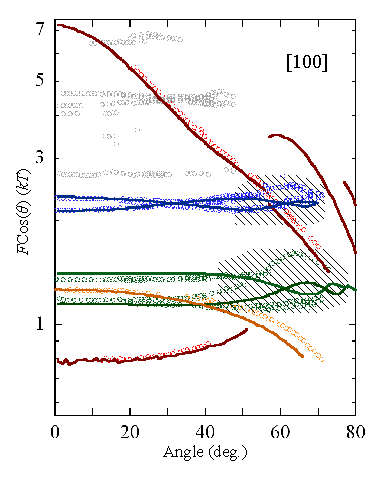
\includegraphics[scale=0.9]{Chapter-dHvABaFe2P2/Figures/AngleDepMeasurements/TightBindingFits/TightBindingFits}
        \caption{Rotation plots for the tight-binding fits calculated from the c-axis down towards $[100]$. As can be seen from the highlighted areas, although the fit residuals are correct to $\sim4\%$, the rotation plot breaks down for high angles in the case of the electron bands.}
        \label{Fig:ResD:TightBindingFitRotationPlot}
    \end{center}
\end{figure}
\begin{table}
    \caption{Harmonic expansion fit parameters performed on the shifted DFT Fermi surfaces}
    \label{Tab:ResD:HarmonicParams}
    \begin{center}
{\small
    \begin{tabular}[htbp]{lrrrr}
\toprule
Factor	& $\alpha$	& $\beta$	& $\gamma$	& $\delta$	\\
\midrule
$k_{00}$	&  1.90796e$^{-1}$	&  2.59538e$^{-1}$	&  2.58282e$^{-1}$	&  1.35031e$^{-1}$	\\
$k_{02}$	& -1.32049e$^{-2}$	& -1.01956e$^{-3}$	&  0		& 0		\\
$k_{04}$	&  9.24279e$^{-4}$	&  4.28603e$^{-4}$	& -1.01085e$^{-2}$	&  1.95065e$^{-3}$	\\
$k_{20}$	&  4.30196e$^{-4}$	& -1.51226e$^{-4}$	& -1.46090e$^{-1}$	& -6.75502e$^{-2}$	\\
$k_{22}$	&  3.23365e$^{-4}$	&  1.91896e$^{-4}$	&  0		& 0		\\
$k_{24}$	& -9.30815e$^{-2}$	& -4.23320e$^{-2}$	&  1.13859e$^{-2}$	& -5.31077e$^{-3}$	\\
$k_{40}$	& -1.64499e$^{-2}$	&  5.02893e$^{-3}$	&  6.15148e$^{-2}$	& -5.70262e$^{-3}$	\\
$k_{42}$	& -1.49159e$^{-2}$	& -7.07858e$^{-3}$	&  0		& 0		\\
$k_{44}$	& -6.14076e$^{-4}$	& -2.86767e$^{-4}$	& -9.49526e$^{-3}$	&  5.28982e$^{-3}$	\\
$k_{60}$	& 0		& 0		& -1.85170e$^{-2}$	& -1.22242e$^{-3}$	\\
$k_{64}$	& 0		& 0		& -9.04247e$^{-4}$	& -2.82851e$^{-4}$	\\
$k_{80}$	& 0		& 0		& -6.79607e$^{-3}$	& -2.22767e$^{-3}$	\\
$k_{84}$	& 0		& 0		&  1.61746e$^{-3}$	& -1.90500e$^{-3}$	\\
$k_{100}$	& 0		& 0		&  1.07007e$^{-2}$	& 0		\\
$k_{104}$	& 0		& 0		&  7.97948e$^{-4}$	& 0		\\
$k_{120}$	& 0		& 0		& -3.89161e$^{-3}$	& 0		\\
$k_{124}$	& 0		& 0		& -1.57292e$^{-3}$	& 0		\\
$k_{140}$	& 0		& 0		& -1.81052e$^{-3}$	& 0		\\
$k_{144}$	& 0		& 0		&  3.81207e$^{-4}$	& 0		\\
$k_{160}$	& 0		& 0		&  3.04268e$^{-3}$	& 0		\\
$k_{164}$	& 0		& 0		&  1.14420e$^{-3}$	& 0		\\
$k_{180}$	& 0		& 0		& -1.07753e$^{-3}$	& 0		\\
$k_{184}$	& 0		& 0		& -4.92181e$^{-4}$	& 0		\\
\bottomrule
    \end{tabular}
}
    \end{center}
\end{table}

% Band 4
% nu_cos_vals = [0 2 4];
% mu_cos_vals = [0 4];
% mu_sin_vals = [2];
% BAND_NUM = 4;
% OUT_FILENAME = 'band4_pseudo_fs.mat';
% P = [0.190795650551417;-0.0132049241203695;0.000924278555081638;0.000430196076110210;0.000323365284403928;-0.0930815369372282;-0.0164499250846804;-0.0149158554339246;-0.000614076088937712];

% Band 3
% nu_cos_vals = [0 2 4];
% mu_cos_vals = [0 4];
% mu_sin_vals = [2];
% BAND_NUM = 3;
% OUT_FILENAME = 'band3_pseudo_fs.mat';
% P = [0.259537885523148;-0.00101956346539010;0.000428602835795347;-0.000151225676919844;0.000191895525922163;-0.0423319597296428;0.00502893573615497;-0.00707857925603053;-0.000286767052816500];

% Band 2
% nu_cos_vals = [0 2 4 6 8 10 12 14 16 18];
% mu_cos_vals = [0 4];
% mu_sin_vals = [];
% BAND_NUM = 2;
% OUT_FILENAME = 'band2_pseudo_fs.mat';
% P = [0.258282295891213;-0.0101085190499327;-0.146089742845922;0.0113858941052011;0.0615148335223954;-0.00949526005728540;-0.0185169711239324;-0.000904247435640945;-0.00679607129328513;0.00161745790960140;0.0107007232759639;0.000797948298873890;-0.00389161131091256;-0.00157292133954998;-0.00180519311058468;0.000381207138913101;0.00304267547098585;0.00114419875689493;-0.00107753360762167;-0.000492181334709838];

% Band 1 
% nu_cos_vals = [0 2 4 6 8];
% mu_cos_vals = [0 4];
% mu_sin_vals = [];
% P = [0.135031574336540;0.00195065231744799;-0.0675502357038337;-0.00531077032608857;-0.00570262272420267;0.00528982052397907;-0.00122242158640231;-0.000282850535526285;-0.00227673928224173;-0.00190499796892254]




\section{Discussion}

The angle dependent \ac{dHvA} measurements presented are of very good quality as evidenced by a number of traits including the presence of second and third harmonics, the hole orbits showing up over a wide angular range and the early onset of oscillations at \unit[6]{T}. The crystal appears to be very clean although there is some evidence of some misaligned domains, for example from some of the Bragg spots doubling up in the \ac{XRD} and multiple peaks observed in the \ac{FFT} at particular angles -- see for example $\alpha$ towards the $[100]$ direction above $\sim 20\degree$ in figure~\ref{Fig:ResD:AngleSweepMeasured}. Nonetheless this does not appear to affect the overall data.




Similar differences between the measured data and calculations were observed for the sister 122 compound SrFe$_2$P$_2$\cite{Analytis2009} and is entirely consistent with results obtained on the entire \BaFePAs series\cite{Shishido2010}. Notably however, the non-nested 122 pnictide compound CaFe$_2$P$_2$ does not show any such differences to the DFT calculations, suggesting that perhaps the shifts in energy may arise from spin-fluctuations.

Orbital character is negligible for s and p orbitals for all bands which confirms ...

Energy shifts for band $2$ are proprtional to the \DzTwo and \DxzDyz characters, implies there may be a link between the \kz scattering and energy enhancements.


It is interesting to note that the DFT applied energy shifts apply to partially nested Fermi surfaces, whereas the large, unested portion of band 2 has zero shift. Other partially nested pnictide materials such as LaFePO\cite{Carrington2009} and SrFe$_{2}$P$_{2}$\cite{Analytis2009} have similar shifts whereas the non-nested, material CaFe$_{2}$P$_{2}$\cite{Coldea2009} matches the DFT calculations well without any rigid energy shift. This correlation between nesting and corrections to the DFT calculation lends weight to the notion that the shifts in the calculation energies are cause by spin fluctuations.





\section{Conslusions}

The \BaFeP crystal and the subsequent angle dependent \ac{dHvA} measurements are of very good quality as evidenced by a number of traits including the presence of second and third harmonics in the \acp{FFT}, the hole orbits showing up over a wide angular range, the early onset of oscillations at \unit{6}{\tesla} and the observation of the Zeeman splitting of the \ac{FFT} peaks. The crystal appears to be a very clean single crystal although there is some evidence of some misaligned domains, for example from some of the Bragg spots doubling up in the \ac{XRD} and multiple peaks observed in the \ac{FFT} at particular angles -- see for example $\alpha$ towards the $[100]$ direction above $\sim 20\degree$ in figure~\ref{Fig:ResD:AngleSweepMeasured}. There are approximately half a dozen separate peaks observed at this location which implies a similar amount of misaligned domain orientations. This misalignment however does not appear to affect the overall data which largely does not resolve the extra domains.

The Fermiology is largely solved by the angle plots with only a few minor ambiguities.  The $F\cos \theta$ angle dependent plots clearly show approximately level curves for the two hole Fermi surfaces demonstrating that $\alpha$ and $\beta$ are approximately two-dimensional. The hole surface, $\gamma$, deviates at high angles and $\delta$ is strongly three dimensional. Although we cannot say for certain whether $\gamma$ is pinched off or not, based on the rigidly shifted \ac{DFT} we expect that the minima to be small but not zero and was not observed due to low frequency noise in the oscillations.

Previous \ac{dHvA} measurements on BaFe$_2$(As$_{0.37}$P$_{0.63}$)$_2$ by Analytis \etal shown in figure~\ref{Fig:ResD:IdentifyingBands} identified the branch of the \ac{dHvA} angle data at around \unit{500}{\tesla} as the neck of the 2D hole pocket. In our own analysis, it made much more sense to attribute this curve to the neck portion of the 3D hole band, with the neck of the 2D pocket being buried in the low frequency noise. These two different statements are not necessarily incompatible. Since the \ac{DFT} data for the entire series suggests that whilst the 2D hole pocket retains the same shape along the \BaFePAs series, the 3D hole pocket narrows considerably at the $\Gamma$ point and switches from being concentric with the 2D pocket at $x=1$ to crossing through the 2D pocket as $x$ is reduced. However when the spin-orbit interaction is considered in the \ac{DFT} calculations, the crossing of the surfaces causes the bands to be redifined such that the bands do not actually cross, in which case there would not be a Yamaji point as specified in the Analytis paper since the similarly sized orbits at \unit{50}{\degree} angle are not from the same band. An attempt was made to see if there was an enhacement of the oscillation amplitude at the correpsonding putative Yamaji point in the \BaFeP data but the close proximity of the strong oscillations from the electron pockets made this intractable with this particular data set.

Although the Fermi surface appears to nest at the $q=(\pi, \pi, \pi/4)$ as shown in figure~\ref{Fig:ExpD:ZSlices}, the correpsonding imaginary part of the susceptibility data shows stronger enchancements at the $q=(\pi, \pi, \pi/2)$ vector, primarily due to the nesting between the 3D hole fermi surface and the inner electron surface. However the susceptibility calculations do not take into account the orbital character of electrons at these nesting vectors. The dominant character at $q=(\pi, \pi, \pi/2)$ is between regions of \DxzDyz on the narrow portion of the 3D surface and regions that switch between \Dxy and \DxzDyz on the electron surface. This will supress the scattering between the two due to considerations of angular momentum. Notheless the susceptibility shows there are significant enhancements of the imaginary part of the susceptibility repsonse between the electron and hole surfaces and the partial nesting conditions required for spin fluctuations are satisfied. Given that that the system becomes more two dimensional as we approach the superconducting region, this suggests that the nesting is enhanced and the fluctuations become stronger.

Like previous measurements of band structure by \ac{dHvA} in the \BaFePAs materials, the Fermi surfaces are smaller than predicted by \ac{DFT} calculations\cite{Shishido2010, Analytis2010c}. Ortenzi \etal~\cite{Ortenzi2009} posits an explanation based on interband scattering which leads to shrinking of the electron and hole pockets and an enhancement of the effective mass based on relaxing an assumption on the chemical potential being far\footnote{i.e. greater than the scattering boson energy scale} from the electron/hole band edges. Similar moderate effective mass enhacements to what we found in \BaFeP of around $1.4m_e$ were calculated --- albeit modeled on a more two dimensional pnictide, LaFePO --- along with the fact that the theory predicts stronger shifts where interband coupling occurs is supported by the \BaFeP data. The nested portions of the 3D $\delta$ hole band, for example, is strongly shifted where it nests with the electron band but the bulge which does not nest with anything is nto shifted at all. Similar shifts between the measured data and calculations were observed for the sister 122 compound SrFe$_2$P$_2$\cite{Analytis2009} which is also a partially nested material and yet shifts are notably absent for the non-nested 122 pnictide compound CaFe$_2$P$_2$~\cite{Coldea2009} which matched the \ac{DFT} calculations with no ajdustments to the energies. 

% Ortenzi's paper is not specific as to the type of scattering other than it is mediated via a bosonic mode with the prime candidates being \ac{SDW}, \ac{CDW} and phonons. \TODO{More here}

It is not clear at this stage whether the shifting of the Fermi surface proprtional to the electron character for the 3D hole $\delta$ band performed in section~\ref{Sec:ResD:ShiftingDFTPropToOrbitalCharacter} represents anything physical or is simply a convenient and reproducable way to obtain the correct band topology. Settling this question will require further investigation. However it is interesting to note that the energy shifts for the 3D hole surface are proprtional to the \DzTwo and \DxzDyz characters, suggesting there may be a link between the $k_z$ scattering component and energy enhancements. Recalling that the 3D hole surface is where we expect to see the the strongest nesting component this also suggest that the scattering between layers may play a part in supressing superconductivity.

The wide bulge in the 3D hole surface ensures that several terms are needed for the harmonic fits represented in section~\ref{Sec:ResD:TightBindingFits}. For this reason, the harmonic fits simply represent a convenient way to obtain the Fermi surface topology in the case of the 3D hole pocket.



\chapter{Hall measurements on \acs{BSCO}}


\section{Sample growth}

The samples were grown by Prof. Takeuchi's group in Sendai University, Japan in May 2009 using the floating zone technique. Here powders of the correct stoichiometry are compacted into a rod and fed slowly through a furnace. A region towards the centre of the furnace heats the powders into a viscous melt, just below this region is a seed crystal. As the end of the rod passes through the melt region, it meets the seed crystal below and solidifies epitaxially onto it. The impurities are held in the melt portion of the crystal by a thermodynamic energy gradient. The rod continues to be slowly passed through the melt region, continually solidifying into the single crystal below until the entire rod has passed through and the growth is over. The end portion, containing the impurities is then removed. Samples from the same growth batch have previously been studied using \ac{ARPES} and \ac{STM} by members of the Sendai group~\cite{Wise2009, Wise2008, Kondo2007, Kondo2005, Kondo2010, Kondo2009, Kondo2006, Kondo2007}.

Table~\ref{Tab:ResH:SampleGrowthDetails} lists the nominal stoichiometries of the samples grown as well as the annealing conditions. Also listed are the \emph{nominal} $T_c$ values for the source crystals which are used to name the samples, the actual measured $T_c$ values of individual samples for the purposes of doping determination are slightly different due to different definitions of $T_c$\footnote{The source crystals were defined based on the zero value $T_c$, the $T_c$ for doping purposes is defined as the mid-point of the transition with an error based on the difference between the mid-point and the zero-point.}.
% \begin{table}
%     \begin{center}
%            \caption{Doping as determined by the Tallon relation, the Ando relation and scaling to \ac{TL2201} data as described in the method section.}
%         \begin{tabular}[htbp]{lrrrr}
% \toprule
% Sample	& $T_c$ ($K$)   & $p_{\textrm{Tallon}}$	& $p_{\textrm{Ando}}$	& $p_{\textrm{Tl}}$	\\
% \midrule
% B00KOD1A	& $0.0\pm1.0$	& $0.270\pm0.003$	& $0.223\pm0.002$	& $0.311\pm0.004$	\\
% B07KOD2		& $11\pm3.8$	& $0.252\pm0.013$	& $0.212\pm0.008$	& $0.271\pm0.013$	\\
% B16KOD1A	& $17\pm1.0$	& $0.240\pm0.004$	& $0.206\pm0.002$	& $0.249\pm0.004$	\\
% B30KOD3		& $29\pm0.5$	& $0.209\pm0.003$	& $0.188\pm0.002$	& $0.209\pm0.003$	\\
% B32KOP1		& $36\pm1.0$	& $0.160\pm0.018$	& $0.160\pm0.010$	& $0.160\pm0.018$	\\
% B32KOP4		& $35\pm2.0$	& $0.178\pm0.026$	& $0.170\pm0.015$	& $0.178\pm0.026$	\\
% B30KUD3		& $32\pm1.0$	& $0.123\pm0.008$	& $0.139\pm0.005$	& $0.123\pm0.008$	\\
% B28KUD3A	& $31.5\pm1.0$	& $0.121\pm0.008$	& $0.138\pm0.004$	& $0.121\pm0.008$	\\
% \bottomrule
%         \label{Tab:ResH:Dopings}
%         \end{tabular}
%     \end{center}
% \end{table}

\begin{table}
    \begin{center}
           \caption{Growth details for the \ac{BSCO} samples. OD, OP and UD stand for over, optimally and under doped respectively. $T_c$ values are nominal.}
        {\small \begin{tabular}[htbp]{lllllllll}
\toprule
\multicolumn{6}{c}{Nominal composition} & & & \\
Bi  & Pb  & Sr  & La  & Cu  & O   & $T_c$   & Reg.  & Annealing conditions \\
\midrule
1.72    & 0.38  & 1.85  & 0.0   & 1.0   & 6+d   & $<$2  & OD    & \unit{400}{\celsius}, \unit{96}{\hour} in \unit{2.5}{\textrm{atm.}} O$_2$ \\
1.72    & 0.38  & 1.85  & 0.0   & 1.0   & 6+d   & 7     & OD    & \unit{750}{\celsius}, \unit{24}{\hour} in air \\
1.72    & 0.38  & 1.85  & 0.0   & 1.0   & 6+d   & 16    & OD    & \unit{550}{\celsius}, \unit{72}{\hour} in flowing N$_2$ \\
1.35    & 0.85  & 1.47  & 0.38  & 1.0   & 6+d   & 30    & OD    & As grown \\
1.35    & 0.85  & 1.47  & 0.38  & 1.0   & 6+d   & 32    & OP    & \unit{650}{\celsius}, \unit{72}{\hour} in flowing N$_2$ \\
1.2     & 0.90  & 1.30  & 0.55  & 1.0   & 6+d   & 30    & UD    & As grown \\
1.2     & 0.90  & 1.30  & 0.55  & 1.0   & 6+d   & 28    & UD    & \unit{650}{\celsius}, \unit{72}{\hour} in flowing N$_2$ \\
\bottomrule
        \label{Tab:ResH:SampleGrowthDetails}
        \end{tabular}}
    \end{center}
\end{table}

\pagebreak
The samples are named according the convention,
\begin{quote}
\code{B<Tc>K<UD/OP/OD><Crystal No.><Sample No.>}
\end{quote}
where UD/OP/OD stands for underdoped, optimally doped and overdoped respectively. So for example `B00KOD2A' refers to the sample `A' taken from the crystal `B00KOD2' --- the second overdoped crystal with a nominal $T_c$ of $\unit{0}{K}$.

\section{Size determination}

Thicknesses were determined for some of the samples using the \ac{FIB} or the optical microscope as described in the methods section. These measurements were performed with the help of Dr. P. Heard. The thicknesses used to calculate absolute values of $R_H$ are listed in table~\ref{Tab:ResH:Thicknesses} and are marked in grey. \ac{FIB} results are given for areas as close to the two voltage contacts that were visible in the scans. As can be seen in the example scan shown in figure~\ref{Fig:ResH:FIBExamples}, there is some variation in the depth along the sample length.
\begin{figure}[htbp]
	\begin{center}
		\includegraphics[scale=0.9]{Chapter-HallBSCO/Figures/FIBExamples/FIBExamples}
		\caption{Top shows an image composited from several \ac{FIB} scans along the length of sample B00KOD1A, with bottom right showing a detail of the right voltage leg. Bottom left shows an oblique top down view of sample B30KOD3.}
		\label{Fig:ResH:FIBExamples}
	\end{center}
\end{figure}

The two scans shown are of good quality, however for the purpose of estimating errors in the thickness some of the scans presented problems. Samples B26KOD1A, B28KUD3A, B30KOD2 and B30KUD3 were obscured with the grease applied as part of the pulsed field measurements. Other samples were not correctly earthed such as B28KUD3B which made the images dark, whilst samples B07KOD2 and B32KOP3 were very flaky under close scrutiny. A scan of B30KOD3 showed that it was partially split in the ab plane which may contribute to systematic error in thickness estimate. In all these cases, the estimate in the thickness error was adjusted accordingly to compensate. A more comprehensive set of \ac{FIB} scans, including images of the split in the layers can be found in Appendix~\ref{Appendix:FIBScans}.

The oblique view of B30KOD3 in figure~\ref{Fig:ResH:FIBExamples} shows a clear misalignment of the voltage legs to the right of the image. This illustrates why it is necessary to take both positive and negative field sweeps in order to separate the magnetoresistance from the Hall components. This also explains why the length and width determinations were subject to large errors which affects the absolute value of the in-plane resistivity calculations.

\begin{table}
    \begin{center}
           \caption{Sample measurements as determined by optical microscope measurements and thickness as determined by \ac{FIB}. Samples highlighted in grey were used for determining absolute values of $R_H$. A and B refer to each of the two contacts visible to the \acs{FIB} scan.}
        {\small \begin{tabular}[htbp]{lrrrrr}
\toprule
	& \multicolumn{3}{c}{Optical}			& \multicolumn{2}{c}{\acs{FIB}}		\\
Sample  & Length (\unit{\micro\metre})	& Width (\unit{\micro\metre})		& Thick. (\unit{\micro\metre})	& Contact A (\unit{\micro\metre})    & Contact B (\unit{\micro\metre})    		\\

\midrule
\cellcolor[gray]{0.9}B00KOD1A	& \cellcolor[gray]{0.9}$781\pm123$	& \cellcolor[gray]{0.9}$157\pm49$	& \cellcolor[gray]{0.9}N/A		& \cellcolor[gray]{0.9}$45\pm1$	& \cellcolor[gray]{0.9}$50\pm5$	\\
B00KOD1B	& $627\pm49$	& $196\pm44$	& $39\pm5$ 	& $43\pm1.5$	& $45\pm1.5$	\\
B07KOD1		& $1277\pm74$	& $392\pm49$	& $29\pm10$	& N/A		& N/A		\\
\cellcolor[gray]{0.9}B07KOD2		& \cellcolor[gray]{0.9}$1061\pm69$	& \cellcolor[gray]{0.9}$333\pm74$	& \cellcolor[gray]{0.9}N/A		& \cellcolor[gray]{0.9}$20\pm5$ 	& \cellcolor[gray]{0.9}$30\pm1$ 	\\
\cellcolor[gray]{0.9}B16KOD1A	& \cellcolor[gray]{0.9}$795\pm34$	& \cellcolor[gray]{0.9}$299\pm34$	& \cellcolor[gray]{0.9}N/A		& \cellcolor[gray]{0.9}$24\pm1$ 	& \cellcolor[gray]{0.9}$24\pm1$ 	\\
B16KOD2A	& $358\pm29$	& $172\pm54$	& $9\pm1$ 	& N/A		& N/A		\\
B16KOD3		& $1122\pm44$	& $368\pm83$	& N/A		& $25\pm2$ 	& $24\pm2$ 	\\
B30KOD1	 	& $436\pm34$	& $250\pm44$	& $21\pm2$ 	& N/A		& N/A		\\
B30KOD2		& $344\pm44$	& $137\pm29$	& $20\pm5$ 	& $15\pm4$	& $15\pm4$	\\
\cellcolor[gray]{0.9}B30KOD3 	& \cellcolor[gray]{0.9}$255\pm49$	& \cellcolor[gray]{0.9}$98\pm25$ 	& \cellcolor[gray]{0.9}N/A		& \cellcolor[gray]{0.9}$16.5\pm1.5$	& \cellcolor[gray]{0.9}$19\pm1$	\\
\cellcolor[gray]{0.9}B32KOP1 	& \cellcolor[gray]{0.9}$658\pm83$	& \cellcolor[gray]{0.9}$397\pm34$	& \cellcolor[gray]{0.9}N/A		& \cellcolor[gray]{0.9}$6.5\pm1.5$	& \cellcolor[gray]{0.9}$6.5\pm1.5$	\\
B32KOP2		& $441\pm25$	& $226\pm20$	& $10\pm1$ 	& N/A		& N/A		\\
B32KOP3		& $437\pm34$	& $118\pm20$	& N/A		& $6\pm1$ 	& $6\pm1$ 	\\
B32KOP4 	& $427\pm74$	& $137\pm39$	& N/A		& $9\pm3$ 	& $9\pm3$ 	\\
B30KUD1A	& $622\pm49$	& $447\pm25$	& $36\pm3$ 	& N/A		& N/A		\\
B30KUD1B	& $828\pm34$	& $471\pm64$	& $35\pm3$ 	& N/A		& N/A		\\
B30KUD2 	& $545\pm69$	& $152\pm39$	& N/A		& $5 \pm1$ 	& $5 \pm1$ 	\\
\cellcolor[gray]{0.9}B30KUD3 	& \cellcolor[gray]{0.9}$476\pm49$	& \cellcolor[gray]{0.9}$118\pm34$	& \cellcolor[gray]{0.9}N/A		& \cellcolor[gray]{0.9}$7\pm2$ 	& \cellcolor[gray]{0.9}$7\pm2$ 	\\
B28KUD2A	& $657\pm29$	& $250\pm39$	& $11\pm1$ 	& N/A		& N/A		\\
\cellcolor[gray]{0.9}B28KUD3A	& \cellcolor[gray]{0.9}$633\pm49$	& \cellcolor[gray]{0.9}$142\pm34$	& \cellcolor[gray]{0.9}N/A		& \cellcolor[gray]{0.9}$16\pm3$	& \cellcolor[gray]{0.9}$16\pm3$	\\
B28KUD3B	& $653\pm44$	& $216\pm49$	& N/A		& $16\pm3$	& $16\pm3$	\\
\bottomrule
        \label{Tab:ResH:Thicknesses}
        \end{tabular} }
    \end{center}
\end{table}




\section{Doping determination}
    \label{Sec:ResH:DopingDetermination}

As described in section~\ref{Sec:Intro:DeterminingDoping}, we compared the Hall values of our samples at high temperature to determine the doping similar to the method used by Ando \etal\cite{Ando2000}. In order to compare this method with other doping characterisation methods, the actual (i.e. not nominal) $T_c$ values for the samples were used from the resistivity curves shown in figure~\ref{Fig:ResH:TSweeps}. These values were input into the parabolic relation from Presland \etal~\cite{Presland1991} and Ando \etal~\cite{Ando2000}. This is then compared with the doping assignments which we make by matching $R_H(\unit{300}{\kelvin})$ in the \ac{BSCO} data from the previous section with that compiled in Kokalj \etal~\cite{Kokalj2012} on \ac{TL2201}. The results of these comparisons are shown in figure~\ref{Fig:ResH:DopingRh300}.
\begin{figure}[htbp]
    \begin{center}
        \includegraphics[scale=1.1]{Chapter-HallBSCO/Figures/DopingRh300/DopingRh300}
        \caption{Assigning the dopings of the \ac{BSCO} data such that $R_H(\unit{300}{\kelvin})$ values match those of \ac{TL2201}. Dashed line is a second order polynomial fit to the \ac{TL2201} data that is used to obatin the exact dopings.}
        \label{Fig:ResH:DopingRh300}
    \end{center}
\end{figure}
The \ac{TL2201} data does not span the entire range of $R_H(\unit{300}{\kelvin})$ values that the \ac{BSCO} covers, for this reason a second order polynomial is fit to the Kokalj data and the \ac{BSCO} doping is assigned to this curve. The underdoped sample B28KUD3a is far along the extrapolated curve, however still lies within the standard Presland/Tallon assignment as used to determine the dopings for the Konstantanovic data~\cite{Konstantinovic2001}.

Figure~\ref{Fig:ResH:Dopings} shows the dopings as determined by the three different methods outlined in the experimental methods chapter. The dopings of the crystals range from $p=0.12$ to $p=0.36$ hole per Cu atom with significant discrepancies between the methods. The Ando determination bunches the doping values around a much narrower range, whereas the dopings determined by comparing with the \ac{TL2201} \ac{dHvA} data, spread the overdoped values over a wider range. The Presland/Tallon method sits between the two. Most notable is that the dopings assigned by Kondo \etal~\cite{Kondo2004} from \ac{ARPES} measurements of the Fermi surface volume taken at \unit{200}{\kelvin}. These are for different samples from the same growth batch but show significantly higher still span of dopings between $p=0.25$ and $p=0.43$. It is not clear why there is a discrepancy given that both determinations are based measure of the Fermi surface in the normal state (the \ac{dHvA} begin field induced at low temperature and \ac{ARPES} being above $T_c$), however we believe that the \ac{ARPES} data may be subject to some kind of surface charge effect since it shows that the overdoped \unit{0}{\kelvin} sample has passed the van-Hove singularity when our Hall data (obtained from the sample bulk) does not show any evidence for this.

\begin{figure}[htbp]
    \begin{center}
        \includegraphics[scale=1.1]{Chapter-HallBSCO/Figures/Dopings/Dopings}
        \caption{Doping distributions for the three different methods. From left to right, B28KUD3A, B30KUD3 (Assume UD), B32KOP1, B32KOP4, B30KUD3 (Assume OD), B30KOD3, B16KOD1A, B07KOD2, B00KOD1A. Broken lines are a guide to the eye. Circled points are B30KUD3 for both the overdoped and underdoped scenarios.}
        \label{Fig:ResH:Dopings}
    \end{center}
\end{figure}

% \begin{figure}[htbp]
%     \begin{center}
%         \includegraphics[scale=1.2]{Chapter-HallBSCO/Figures/DRhoDtCurves/DRhoDtCurves}
%         \caption{$d\rho(T)/dT$ curves for each of the samples taken in \unit{0}{\tesla} and \unit{13}{\tesla} field. Note the evolution of the $T_{\textrm{coh}}$ gradient in the overdoped samples which give way to the $T^*$ kink in the underdoped samples, B30KUD3 has been repositioned to follow this trend.}
%         \label{Fig:ResH:DRhoDtCurves}
%     \end{center}
% \end{figure}
% The derivatives of the same resistivity curves in figure~\ref{Fig:ResH:TSweeps} are plotted in figure~\ref{Fig:ResH:DRhoDtCurves} along with derivatives to temperature sweeps taken at \unit{13}{\tesla}. Here we can see in the overdoped samples the distinct slope downwards towards \Tc which signifies the coherent quasiparticle region which begins at $T_{\textrm{coh}}$. This gradually levels out as doping is reduced until we observe a kink which marks the pseudogap temperature, $T^*$. The $T^*$ kink is weaker in B30KUD3 than the optimally doped samples and in fact only appears, at a much lower temperature, when the field is applied. This suggests that it is in fact more doped than the optimally doped samples rather than less doped as the nominal composition would suggest. If we consider B30KUD3 to be overdoped rather than underdoped then this trend continues right across the range of samples.


% Figure~\ref{Fig:ResH:Rh300Comparison} present Hall data at \unit{300}{\kelvin} again taken in the Polo with comparable data from Konstantinovi\'c \etal~\cite{Konstantinovic2001}.
% \begin{figure}[htbp]
%     \begin{center}
%         \includegraphics[scale=1.1]{Chapter-HallBSCO/Figures/Rh300Comparison/Rh300Comparison}
%         \caption{Hall data at \unit{300}{\kelvin} compared with similar data taken from refs.~\cite{Konstantinovic2001, Kokalj2012} using different doping assignments. From left: Tallon relation, Ando relation and scaling to \ac{TL2201} data. Red lines are guides to the eye, circled points are B30KUD3 in the overdoped and underdoped positions.}
%         \label{Fig:ResH:Rh300Comparison}
%     \end{center}
% \end{figure}
% It is clear that the Ando assignment of dopings is too confined with the data not at all following the respective curves whereas the Tallon relation follows much close the shape of the curve, although, perhaps this is not surprising given that the dopings in the Konstantinovo\'c paper were also assigned using the Tallon relation. However what is most interesting is that when compared with \ac{TL2201} data from Kokalj \etal~\cite{Kokalj2012} which we know is appropriate to scale to the \ac{TL2201} doping scheme, we see that of the three methods, scaling the \ac{BSCO} to the \ac{TL2201} \ac{dHvA} data matches the closest. On this rationale, we continue assuming that the \ac{TL2201} doping assignments are the correct ones.

% Also, referring to the circled points, we see that again the data is more consistent if we consider the B30KUD3 to be overdoped rather than underdoped. Looking back to the inset of figure~\ref{Fig:ResH:TSweeps} we see that there is large scatter in the data points due to uncertainty in the dimensions which were determined by optical microscope, however there is an approximate downward trend with doping which is similar to what is found in the literature~\cite{Ando2000, Ando1999, Konstantinovic2001, Ono2000}. Although B30KUD3 is more consistent to this trend in the underdoped position, the trend still lies with the error bars of the overdoped position. Looking ahead to the inset of figure~\ref{Fig:ResH:InvHallCombined} which shows $R_H$ values at \unit{300}{\kelvin} vs. doping, which depend only on the measurement of depth --- which was much more accurately determined by the \ac{FIB} --- we see that the underdoped position lies far outside the overall trend even when considering the error bars. 



\section{Temperature sweeps}

Figure~\ref{Fig:ResH:TSweeps} shows the in-plane resistivity, $\rho(T)$ for each of the samples in zero field taken in the \ac{VTI} in the Polo magnet. From this plot we can characterise the \Tc of the samples and find the residual resistivity, $\rho_0$ by using simple linear fits to the data above the transition temperatures and extrapolate back to zero. Table~\ref{Table:ResH:TSweepFitsParams} show the fit parameters for each of the samples. 
\begin{table}
	\begin{center}
       	\caption{Fits parameters to $\rho = \rho_0 + \rho_1T$ for zero field resistivity data above $T_c$ as well as $T_c$ values determined from the same plots. Fits at low $T$ are shown in inset to figure~\ref{Fig:ResH:TSweeps}.}
		{\small \begin{tabular}[htbp]{lrrrr}
\toprule
Sample		& $\rho_0 (\unit{\micro\ohm\centi\metre})$	& $\rho_1 (\unit{\micro\ohm\centi\metre})$  & $T_c$ (\unit{\kelvin})	& $T_c/T_c(\textrm{max})$	\\
\midrule
B00KOD1A	& 40.7		& 0.454     & $0\pm1.0$	    & $0.00\pm0.03$	\\
B07KOD2		& 73.0		& 1.026     & $11\pm3.8$	& $0.31\pm0.11$	\\
B16KOD1A	& 49.9		& 0.843     & $17\pm1.0$	& $0.47\pm0.03$	\\
B30KOD3		& 15.9		& 0.578     & $29\pm0.5$	& $0.81\pm0.01$	\\
B32KOP1		& 54.2		& 0.824     & $36\pm1.0$	& $1.00\pm0.03$	\\
B32KOP4		& 55.6		& 1.904     & $35\pm2.0$	& $0.97\pm0.06$	\\
B30KUD3		& 123.0		& 2.233     & $32\pm1.0$	& $0.89\pm0.03$ \\
B28KUD3A	& 22.6		& 0.806     & $32\pm1.0$	& $0.89\pm0.03$	\\
\bottomrule
		\label{Table:ResH:TSweepFitsParams}
		\end{tabular} }
	\end{center}
\end{table}
The residual resistivities are very good with only one being above \unit{100}{\micro\ohm\centi\metre} and most below \unit{70}{\micro\ohm\centi\metre} which has been cited as being exceptionally good for \ac{BSCO}~\cite{Ando1999}. Moreover the \Tc of the optimally doped sample is \unit{36}{\kelvin} which is amongst the highest reported~\cite{Ando1999} which again is testament to the crystal quality. $\rho_0$ generally increases as you move away from critical doping which lends support to the notion of the La doping increasing the disorder in the CuO layers.

The inset to figure~\ref{Fig:ResH:TSweeps} shows the $\rho(\unit{300}{\kelvin})$ values for the samples along with error bars due to uncertainty in the size determination. As we saw in the previous section, there is significant misalignment and overall width to the voltage contacts which lead to large systematic errors which affect scaling only. Nonetheless, there appears to be an downward trend in resistivity as doping is increased. The circled points are B30KUD3 in both the overdoped and underdoped position and although the position is perhaps more fitting in the underdoped position, there error bars leave the overdoped point well within the overall trend.


% \begin{table}
% 	\begin{center}
%        	\caption{Fits parameters to $\rho = \rho_0 + \alpha_1T +
%        	\alpha_2T^2$ for zero field resistivity data above $T_c$.
%        	Fits at low $T$ are shown in inset to figure~\ref{Fig:ResH:TSweeps}}
% 		\begin{tabular}[htbp]{lrrr}
% \toprule
% Sample		& $\rho_0 (\times10^-2)$	& $\alpha_1 (\times10^{-4})$	& $\alpha_2 (\times10^{-7})$	\\
% \midrule
% B00KOD1A	& 12.26		& 6.895		& 14.394		\\
% B07KOD2		& 9.03		& 7.740		& 8.459			\\
% B16KOD1a	& 4.25		& 4.809		& 3.610			\\
% B30KOD3		& 1.43		& 3.385		& 4.595			\\
% B32KOP1		& 1.20		& 2.596		& -0.810		\\
% B32KOP4		& 2.76		& 21.886	& -8.862		\\
% B30KUD3		& 18.80		& 38.028	& -4.385		\\
% B28KUD3a	& 2.71		& 18.447	& -6.756		\\
% \bottomrule
% 		\label{Table:ResH:TSweepFitsParams}
% 		\end{tabular}
% 	\end{center}
% \end{table}


\section{Hall plots}

Figures~\ref{Fig:ResH:HallIndividualOD}, \ref{Fig:ResH:HallIndividualOP} and \ref{Fig:ResH:HallIndividualUD} show the Hall coefficients extracted as described in the methods section for samples progressing from overdoped, optimally doped to underdoped respectively. Where appropriate, the data is compared to that from Ando \etal~\cite{Ando1999}. Red lines in the plots are guides to the eye.

For the samples of $T_C >= \unit{28}{\kelvin}$ there are some data which did not reach sufficient field to obtain linear behaviour which are circled with a dashed line in the plots. For sample B30KOD2, many of the sweeps for $T < \unit{45}{\celsius}$ showed significant hysteresis due to temperature drift. Despite temperature correction, many of the fits did not pass through the origin (circled in the figure) which is a good indicator that the true field suppressed linear Hall has not been obtained. The same goes for the circled points on the B30KUD2 plot and another data point at $T=\unit{1.5}{\kelvin}$ and $R_H = \unit{$7.3\times10^{-3}$}{\centi\metre\cubed}$ from the first trip to \ac{LNCMI} which is outside the plot boundary as well as data points on the plot for B28KUD3B. The data sets are combined, minus the points highlighted in the previous paragraph, in the main panels of figure~\ref{Fig:ResH:InvHallCombined} alongside the data from the Ando paper.

\begin{figure}[htbp]
	\begin{center}
		\includegraphics[scale=0.9]{Chapter-HallBSCO/Figures/HallIndividual/HallIndividualOD}
		\caption{$R_H$ for underdoped samples of \ac{BSCO}. Plots show results from, $\bullet$ Polo in June 2010, $\blacktriangle$ \ac{LNCMI} in June 2009, $\blacktriangledown$ \ac{LNCMI} in Feb 2010, $\blacksquare$ Nijmegen in May 2010. Symbols for comparable samples are marked on the plots. Red lines are a guide to the eye.}
		\label{Fig:ResH:HallIndividualOD}
	\end{center}
\end{figure}

\begin{figure}[htbp]
	\begin{center}
		\includegraphics[scale=0.9]{Chapter-HallBSCO/Figures/HallIndividual/HallIndividualOP}
		\caption{$R_H$ for underdoped samples of \ac{BSCO}. Plots show results from, $\bullet$ Polo in June 2010, $\blacktriangle$ \ac{LNCMI} in June 2009, $\blacktriangledown$ \ac{LNCMI} in Feb 2010, $\blacksquare$ Nijmegen in May 2010. Symbols for comparable samples are marked on the plots. Dashed lines indicate points where the field was not sufficient to achieve linear behaviour. Red lines are a guide to the eye.}
		\label{Fig:ResH:HallIndividualOP}
	\end{center}
\end{figure}

\begin{figure}[htbp]
	\begin{center}
		\includegraphics[scale=0.9]{Chapter-HallBSCO/Figures/HallIndividual/HallIndividualUD}
		\caption{$R_H$ for underdoped samples of \ac{BSCO}. Plots show results from, $\bullet$ Polo in June 2010, $\blacktriangle$ \ac{LNCMI} in June 2009, $\blacktriangledown$ \ac{LNCMI} in Feb 2010, $\blacksquare$ Nijmegen in May 2010. Symbols for comparable samples are marked on the plots. Dashed lines indicate points where the field was not sufficient to achieve linear behaviour. Red lines are a guide to the eye.}
		\label{Fig:ResH:HallIndividualUD}
	\end{center}
\end{figure}
\begin{figure}[htbp]
	\begin{center}
		\includegraphics[scale=1.1]{Chapter-HallBSCO/Figures/InvHallCombined/InvHallCombined}
		\caption{Hall data in context with data from Ando \etal\cite{Ando1999} (open circles) which are in order of increasing $R_H$, 24KOD, 30KOD, 33KOP, 28.5KUD, 20KUD. Right panel shows the inverse hall data which relates to carrier density. Red lines are the same guides to the eye used in previous figures. Inset shows $R_H$ at \unit{300}{\kelvin} plus systematic error bars due primarily to uncertainty in thickness vs. doping scaled to \ac{TL2201} data. B30KUD3 (circled) is plotted in both the overdoped and underdoped positions.}
		\label{Fig:ResH:InvHallCombined}
	\end{center}
\end{figure}

With reference to figure~\ref{Fig:ResH:InvHallCombined} and in particular the new low temperature data points, we see that doping strongly affects the qualitative shape of the $R_H$ curves. Whilst the trend appears to be that $R_H(\unit{300}{\kelvin})$ decreases as doping increases as to be expected, the $R_H(\unit{0}{\kelvin})$ values all tend toward approximately similar values of around \unit{$0.5\times 10^{-3}$}{\centi\metre\cubed}to \unit{$1.5\times 10^{-3}$}{\centi\metre\cubed}. The most pronounced difference between high and low temperature values though is with the optimally doped samples which are around $\times 2.75$ greater at high temperature. Right down to \unit{0}{\kelvin} there is no sign change in $R_H$, which suggests that the hole pockets have higher mobility than the electron pockets across the range of dopings studied.

The error bars on the data points do not include error from the thicknesses which are systematic across the data points. The inset of figure~\ref{Fig:ResH:InvHallCombined} shows the $R_H$ values at \unit{300}{\kelvin} vs. doping for each of the samples with these error bars applied. The overall trend is downward with doping with the progression being approximately monotonic, however the exception is B16KOD1A which has a slightly lower $R_H$ than would be expected from a linear trend.

The Hall angle is plotted for each of the samples where $B=\unit{0}{\tesla}$ in-plane resistivity data is available in figure~\ref{Fig:ResH:HallAngle} with temperature raised to a fitted exponent, $\alpha$. In the original Chien analysis, $\alpha = 2$ but is allowed to vary here to observe deviations from the expected $T^2$ behaviour. Similar analysis was performed for resistivity data taken at $B=\unit{13}{\kelvin}$ and although these plots are not shown, the fitted $\alpha$ values are plotted in the bottom left subplot along with the $B=\unit{0}{\tesla}$ values. A nominal unitary field was used when calculating $\cot\theta_H$ and only data above the superconducting transition was fitted and is shown in the plots. Note that for the $B=\unit{13}{\tesla}$ case, the Hall data for the optimally doped sample B32KOP1 was compared with resistivity data for sample B32KOP4 which explains the slightly different doping value assigned to it. In this particular instance, it appears that the assignment of the sample B30KUD3 would be more suited to underdoped rather than overdoped.

\begin{figure}[htbp]
    \begin{center}
        \includegraphics[scale=1.0]{Chapter-HallBSCO/Figures/HallAngle/HallAngle}
        \caption{Hall angle calculated with a nominal field of unity from resistivity data taken in zero field. Plot in bottom left shows the fitted exponent, $\alpha$, vs. doping compared with similar data on \ac{BSCO} from Konstantanovi\'c \etal~\cite{Konstantinovic2000} for both zero field resistivity data and resistivity data taken at \unit{13}{\kelvin} ($\cot\theta_H$ plots for $B=\unit{13}{\tesla}$ not shown)}
        \label{Fig:ResH:HallAngle}
    \end{center}
\end{figure}
With reference to the plot in the lower left, the fitted exponents approximately follow the same downward trend with doping as in \ac{BSCO} data from Konstantanovi\'c \etal~\cite{Konstantinovic2000} up to around $p=0.27$. In particular the $B=\unit{13}{\tesla}$ follows the curve reasonably closely before the upturn at $p=0.31$. Downward deviation from the $T^2$ behaviour at high temperatures (as indicated from a drop in the $\alpha$ exponent) at this point in the phase diagram has been previously interpreted to be due to the saddle point in the \ac{DOS} which is approaching from below the Fermi energy~\cite{Ando2004} which would also explain why there is a recovery toward $T^2$ behaviour between $p=0.27$ and $p=0.31$ as the flat portion of the \ac{DOS} passes above the Fermi energy. This would suggest that the van-Hove singularity peaks in the \ac{BSCO} phase diagram at around $p=0.25$, approximately where the B16KOD1A sample lies and where the room temperature $R_H$ value was also found to be slightly lower than expected. However this occurs at a higher doping than the Hashimoto paper would suggest~\cite{Hashimoto2008} (see figure~\ref{Fig:Intro:VanHoveBSCOLSCO}) and given the proximity of the van-Hove singularity, the low Hall coefficient should not be interpreted a simple indicator of carrier density. 
\begin{figure}[htbp]
    \begin{center}
        \includegraphics[scale=0.8]{Chapter-HallBSCO/Figures/RhRatios/RhRatios}
        \caption{Left shows ratio of $R_H$ values at the maximum of the Hall curves and at $T=\unit{0}{\kelvin}$ to the $T=\unit{300}{\kelvin}$ $R_H$ values. Errors in $R_H(\unit{0}{\kelvin}$ estimated from Hall plots, the value for B30KUD2 is estimated based on linear extrapolation. Right shows the temperature where the maximum $R_H$ occurs.}
        \label{Fig:ResH:RhRatios}
    \end{center}
\end{figure}

An alternate explanation based on the Narduzzo paper~\cite{Narduzzo2008} goes as follows. For $p \gtrsim 0.19$, $R_H(\unit{0}{\kelvin} > R_H(\unit{300}{\kelvin})$ as illustrated in figure~\ref{Fig:ResH:RhRatios}. If we assume there is not temperature dependent change of the Fermi surface such that would affect $\vect{v_F}$, then this can be explained by an temperature dependent increase in the anisotropy of the scattering. As detailed in the introduction, such scattering is thought to originate in the overdoped side of the phase diagram and is seemingly closely tied to superconductivity. The Narduzzo paper explores this possibility but ultimately could not definitively conclude that the scattering rate is proportional to $\cos^2(2\phi)$ as is the case in the Abdel-Jawad paper~\cite{Abdel-Jawad2007}.

When we consider the ratio of the maximum $R_H$ to the \unit{300}{\kelvin} value also plotted in figure~\ref{Fig:ResH:RhRatios} then we see that these values do not vary much at all with doping indicating that the scattering process that suppresses the low temperature Hall values only becomes dominant below the temperature where $R_H(\textrm{max})$ occurs. Moreover we note that the low temperature behaviour of $R_H$ which, although not possible to ascertain for certain due to the scatter in points, appears linear in temperature below $R_H(\textrm{max})$, which suggests that the same process explored above is $T$-linear in behaviour. Finally the temperatures of the maximums in $R_H$ are plotted in figure~\ref{Fig:ResH:RhRatios} and show a similar doping behaviour to the $\alpha$ fitted exponents.




% There seems to be little evidence of the transition of the doping from $p$ to $1+p$ which agrees with the notion that these dopings lie beyond where the change in the size of the Fermi surface is thought to take place~\cite{LeBoeuf2007}. 

%Divergence in resistivity occurs beyond UD 0K\cite{Ando2000}, well
%below our lowest nominal doping of ...

% Residual resistivity of ~20\mu\Ohm cm at optimal doping is very small
% and increases with La doping i.e. as become more underdoped
% \cite{Ando2000}





\section{Conclusions}

High quality crystals of Pb and Sr doped \ac{BSCO} were sourced and studied in the normal state by high-field magnetotransport measurements down to low temperatures, thereby determining the low temperature Hall behaviour. The samples exhibited a sharp change in in the $R_H(\unit{0}{\kelvin})/R_H(\unit{300}{\kelvin})$ which coincides with various phenomena related to the pseudogap. This occurs in the field induced normal state which suggests that the scenario described in section~\ref{Sec:Intro:Pseudogap} where the pseudogap disappears at the top of the superconducting dome is not the correct one.

The data was modeled using a simple anisotropic model based on the Ong construction and was found to fit the relative scattering rates in the reasonably well it although consistently underestimated the residual resistivity term and for the overdoped samples overestimated the $T^2$ term. An increase in the $T$-linear term was observed to scale with doping similar to as found by Abdel-Jawad \etal~\cite{Abdel-Jawad2007}. This relatively crude model suggests that with further refinement it could be used to explain the physics at underdoped side of the phase diagram without resorting to complex Fermi surface reconstruction scenarios proposed by LeBeouf \etal The first port of call for the refinement would be the inclusion of the Fermi velocity in the scattering rate which may also improve the agreement in the overdoped side.

A novel doping determination technique is presented based on the method outlined by Ando \etal{} but comparing the \ac{BSCO} samples to the recently determined doping in overdoped \ac{TL2201} using \ac{dHvA}. The method assigns doping values that fall between the `universal' method of Presland/Tallon and those found from \ac{ARPES} measurements by Kondo \etal

A natural continuation of this work would include a more precise determination of the low field region to determine with more certainty if the low temperature behaviour is truly $T$-linear or it plateaus at very low temperatures as found by Balkirev \etal{} in underdoped samples~\cite{Balakirev2003} and then attempt to model it using the Ong construction.




% \chapter{Magnetoresistance measurements on \BSCO}


\section{Temperature sweeps}




\section{Field Sweeps}




\section{Conclusions}





% Bibliography
\clearpage

\thebibliography


% Appendix here

\appendix


\chapter{\BaFeP Band Character}
\label{Appendix:BandCharacter110Slices}

\begin{figure}[h!]
    \begin{center}
        \includegraphics[scale=0.7]{Chapter3-dHvABaFe2P2/Figures/AngleDepMeasurements/BandCharacterPlot/Band1_110Slice_BandCharacter}
        \caption{Orbital character for band 1 taken across a $[110]$ slice of the Brillouin zone}
        \label{Fig:Appendix:BandCharacter110Band1}
    \end{center}
\end{figure}
%%
\begin{figure}[h!]
    \begin{center}
        \includegraphics[scale=0.7]{Chapter3-dHvABaFe2P2/Figures/AngleDepMeasurements/BandCharacterPlot/Band3_110Slice_BandCharacter}
        \caption{Orbital character for band 3 taken across a $[110]$ slice of the Brillouin zone}
        \label{Fig:Appendix:BandCharacter110Band3}
    \end{center}
\end{figure}
%%
\begin{figure}[h!]
    \begin{center}
        \includegraphics[scale=0.7]{Chapter3-dHvABaFe2P2/Figures/AngleDepMeasurements/BandCharacterPlot/Band4_110Slice_BandCharacter}
        \caption{Orbital character for band 4 taken across a $[110]$ slice of the Brillouin zone}
        \label{Fig:Appendix:BandCharacter110Band4}
    \end{center}
\end{figure}


\chapter{`Microfit' parameters}
\label{Appendix:MicroFitParams}

Fit parameters for the `microfitting' technique described in section~\ref{Sec:Exp:LKMicrofitting}. Note: at \unit{46}{\degree} the peak is twinned.

% \begin{table}
    \begin{center}
        % \caption{Fit parameters for the `microfitting' technique described in section~\ref{Sec:Exp:LKMicrofitting}. Note: at \unit{46}{\degree} the peak is twinned.}
        {\small \begin{tabular}[!h]{lllll}
\toprule
Angle (deg.)    & Band      & Frequency (\unit{T})  & Fit Periods   & Filter Range \\
\midrule
12              & $\alpha_1$& 1210                  & 1.5           & 1100--1240     \\
28              & $\alpha_1$& 1269                  & 1.5           & 1200--1310     \\
46              & $\alpha_1$& 1532                  & 1.5           & 1430--1585     \\
12              & $\alpha_2$& 1372                  & 1.5           & 1320--1440     \\
28              & $\alpha_2$& 1530                  & 1.5           & 1450--1650     \\
46              & $\alpha_2$& 2017                  & 1.5           & 1970--2100     \\
28              & $\beta_2$ & 1365                  & 1.5           & 1320--1440     \\
12              & $\beta_1$ & 2180                  & 1.5           & 2100--2270     \\
12              & $\beta_2$ & 2500                  & 1.5           & 2450--2550     \\
28              & $\beta_2$ & 2605                  & 1.5           & 2555--2670     \\
46              & $\beta_2$ & 3347                  & 1.5           & 3250--3370     \\
46              & $\beta_2$ & 3381                  & 1.5           & 3365--2500     \\
12              & $\beta_3$ & 2350                  & 1.5           & 2270--2450     \\
28              & $\beta_3$ & 2475                  & 1.5           & 2400--2560     \\
46              & $\beta_3$ & 2970                  & 1.5           & 2850--3100     \\
12              & $\delta$  & 1270                  & 1.5           & 1250--1310     \\
46              & $\delta$  & 1626                  & 1.5           & 1590--1690     \\
28              & $\gamma_1$& 912                   & 1.5           & 850--970       \\
46              & $\gamma_1$& 1320                  & 1.5           & 1270--1370     \\
46              & $\gamma_2$& 4497                  & 1.5           & 4400--4600     \\
\bottomrule

        \label{Table:Appendix:MicroFitParams}
        \end{tabular} }
    \end{center}
% \end{table}


\chapter{Lindhard susceptibility calculation code}

The following is MATLAB code known to run on release 2008b.

\footnotesize
\lstset{language=Matlab}
\lstinputlisting{Misc/calc_x0.m}
\normalsize


\section{A Comparison of Fermiology Techniques}
\label{Appendix:FermiologyTechniques}



\chapter{\ac{FIB} scans}

Exemplary images from the \ac{FIB} scans performed with the help of Dr. P. Heard.
\begin{figure}[htbp]
	\begin{center}
		\includegraphics[scale=0.7]{Appendices/Figures/FIBScans/FibScans}
		\caption{}
		\label{Fig:App:FibScans}
	\end{center}
\end{figure}
\begin{figure}[htbp]
	\begin{center}
		\includegraphics[scale=0.7]{Appendices/Figures/FIBScans/FibScans2}
		\caption{}
		\label{Fig:App:FibScans2}
	\end{center}
\end{figure}




\end{document}
